\documentclass[times, utf8, diplomski, numeric]{fer}
\usepackage{booktabs}
\usepackage{tabu, multirow}
\usepackage{tabularx}
\usepackage{float}
\usepackage{pdfpages}
% \usepackage{hyperref}
\usepackage{listings}
\usepackage{tikz}
\usepackage{pgfplots}
\usepackage[acronym,nomain]{glossaries}
% \usepackage[automake]{glossaries-extra}

\usetikzlibrary{trees}

\makeglossaries

% \renewcommand{\glsxtrpostdescacronym}{%
%  \ifglshasfield{\glsxtruserfield}{\glscurrententrylabel}%
%  { (\glscurrentfieldvalue)}%
%  {}%
% }
%
% \setabbreviationstyle[acronym]{long-short-user}

\newacronym{smp}{SMP}{Symmetric Multiprocessing}
\newacronym{amp}{AMP}{Asymmetric Multiprocessing}
\newacronym{pl}{PL}{Programmable Logic}
\newacronym{ps}{PS}{Processing System}
\newacronym{sdk}{SDK}{Software Development Kit}
\newacronym{cpu}{CPU}{Central Processing Unit}
\newacronym{apu}{APU}{Application Processing Unit}
\newacronym{scu}{SCU}{Snoop Control Unit}
\newacronym{acp}{ACP}{Accelerator Coherency Port}
\newacronym{dap}{DAP}{Debug  Access  Port}
\newacronym{mmu}{MMU}{Memory Management Unit}
\newacronym{jtag}{JTAG}{Joint Test Action Group}
\newacronym{qspi}{QSPI}{Quad Serial Peripheral Interface}
\newacronym{wfe}{WFE}{Wait For Event}
\newacronym{fsbl}{FSBL}{First Stage Bootloader}
\newacronym{ssbl}{SSBL}{Second Stage Bootloader}
\newacronym{tlb}{TLB}{Translation Look-aside Buffers}
\newacronym{rsapss}{RSA-PSS}{Rivest, Sharim andAdleman - Probabilistic Signature Scheme}
\newacronym{puk}{PuK}{Public Key}
\newacronym{aes}{AES}{Advanced EncryptionStandard}
\newacronym{hmac}{HMAC}{Key-hash message authentication code}
\newacronym{ocm}{OCM}{On Chip Memory}
\newacronym{ram}{RAM}{Random Access Memory}
\newacronym{ppi}{PPI}{Private Peripheral Interrupt}
\newacronym{sgi}{SGI}{Software Generated Interrupt}
\newacronym{irq}{IRQ}{Interrupt Request}
\newacronym{fiq}{FIQ}{Fast Interrupt Request}
\newacronym{spi}{SPI}{Shared Peripheral Interrupt}
\newacronym{gic}{GIC}{Generic Interrupt Controller}
\newacronym{uart}{UART}{Universal Asynchronous Receiver Transmitter}
\newacronym{imei}{IMEI}{International Mobile Equipment Identity}
\newacronym{dma}{DMA}{Direct Memory Access}
\newacronym{dmac}{DMAC}{Direct Memory Access Controller}
\newacronym{tzpc}{TZPC}{TrustZone Protection Controller}
\newacronym{tzasc}{TZASC}{TrustZone Address Space Controller}
\newacronym{tzma}{TZMA}{TrustZone Memory Adapter}
\newacronym{apb}{APB}{Advanced Peripheral Bus}
\newacronym{smc}{SMC}{Secure Monitor Call}
\newacronym{rtos}{RTOS}{Real-Time Operating System}
\newacronym{gpos}{GPOS}{General Purpose Operating System}
\newacronym{vmcb}{VMCB}{Virtual Machine Control Block}
\newacronym{ttc}{TTC}{Triple Timer Counter}
\newacronym{fifo}{FIFO}{First In First Out}
\newacronym{dtc}{DTC}{Device Tree Compiler}
\newacronym{nfs}{NFS}{Network File System}
\newacronym{vfp}{VFP}{Vector Floating Point}
\newacronym{bsp}{BSP}{Board Support Package}
\newacronym{fpu}{FPU}{Floating Point Unit}

\begin{document}

\tikzstyle{every node}=[anchor=west]
\lstset{language=c, xrightmargin=0.001\textwidth}
\pgfplotsset{width=400pt, height=200pt, compat=1.15}

\glsunsetall

\renewcommand{\labelitemi}{$\bullet$}
\renewcommand{\labelitemii}{$-$}
\renewcommand{\betweenauthors}{, }

% TODO: Navedite broj rada.
% \thesisnumber{1995}
%
% % TODO: Navedite naslov rada.
% \title{Proširenje LTZVisor monitora virtualnih strojeva \\za višejezgrene procesore}
%
% % TODO: Navedite vaše ime i prezime.
% \author{Magdalena Halusek}
%
% \maketitle
%
% % Ispis stranice s napomenom o umetanju izvornika rada. Uklonite naredbu \izvornik ako želite izbaciti tu stranicu.
% % \izvornik
% \includepdf[pages=-,pagecommand={}]{0688_001.pdf}

% Dodavanje zahvale ili prazne stranice. Ako ne želite dodati zahvalu, naredbu ostavite radi prazne stranice.
\zahvala{
\\
Zahvaljujem se mentoru, prof. dr. sc. Mariju Cifreku, na slobodi izbora teme diplomskog rada i asistentici
Ivani Čuljak, mag. ing., na dostupnosti i pomoći oko pisanja teksta diplomskog rada. Posebno se zahvaljujem profesoru
Sandru Pintu koji mi je uz ideju za ovaj rad, dao i mnoštvo korisnih savjeta i komentara koji doprinose vrijednosti ovog rada.
Hvala mojim roditeljima, sestrama, bakama, teti, djedu, dečku i prijateljima na potpori koju su mi pružali tijekom
studija i hvala dragome Bogu koji me je nosio kad je bilo teško.}

\tableofcontents

\chapter{Uvod}
Neke od važnih odrednica ugradbenih računala su pouzdanost, predvidljivost i rad u stvarnom vremenu.
Povećanjem popularnosti IoT (engl. \textit{Internet of Things}) uređaja u industriji, počinje se isticati
još jedna dodatna karakteristika, a radi se o sigurnosti uređaja. Kako bi se uređaji u industriji osigurali,
ARM već dugi niz godina daje podršku Cortex-A procesorima \textit{TrustZone} sigurnosnim ekstenzijama.
Izlaskom M profila nove ARMv8 arhitekture, pojavila se i posebno razvijena \textit{TrustZone-M} sigurnosna
podrška Cortex-M procesora. Iako je \textit{TrustZone-M} sigurnosna ekstenzija razvijena ispočetka konkretno
za mikrokontrolere, krajnja funkcionalnost je slična onoj koju pruža \textit{TrustZone} ekstenzija Cortex-A
procesora.\\
U ovom radu bit će opisana \textit{TrustZone} sigurnosna ekstenzija ZedBoard platforme koja implementira
Cortex-A9 procesor s dvije jezgre te sustavom za procesiranje (engl. \textit{Processing System}, \gls{ps}) i programabilnom
logikom (\gls{pl}). Kao primjer maksimalnog iskorištenja \textit{TrustZone} sigurnosne
ekstenzije, bit će prikazan LTZVisor monitor virtualnih strojeva (engl. \textit{hypervisor} ili engl.
\textit{Virtual Machine Monitor}). LTZVisor omogućuje virtualizaciju u ugradbenim računalima, odnosno konkurentno
izvođenje dva operacijska sustava na jednoj jezgri procesora. Pojavom IoT uređaja u industriji, pojavila
se i sve veća potreba za virtualizacijom zbog potrebe za karakteristikama operacijskih sustava za rad u stvarnom
vremenu i operacijskih sustava opće namjene. Specifičnije, karakteristike operacijskog sustava za rad u
stvarnom vremenu koje su potrebne su odziv u stvarnom vremenu, determinizam i pouzdanost. Operacijski
sustav opće namjene je često tražen zbog dobre mrežne podrške koju nudi.\\
U nastavku će biti opisano kako
\textit{TrustZone} doprinosi izolaciji između navedenih operacijskih sustava. Pošto je LTZVisor monitor
virtualnih strojeva namijenjen jednoj jezgri procesora, u ovom radu će se opisati postupak prilagođenja
LTZVisora za obje jezgre ZedBoarda kako bi se maksimalno iskoristile mogućnosti platforme.

\chapter{Arhitektura Cortex-A9 procesora}
\gls{apu} (engl. \textit{Application Processing Unit}) Zynq-7000 platforme može sadržavati jednu ili dvije jezgre, odnosno jedan
ili dva Cortex-A9 procesora \cite{zynq_trm}. ZedBoard sadrži dva Cortex-A9 procesora \textit{little-endian} arhitekture s
koprocesorskom podrškom u višejezgrenoj konfiguraciji. Dva \gls{cpu}-a dijele \textit{cache} memoriju druge razine,
odnosno L2 \textit{cache} memoriju, od 512~kB.
Oba procesora su visokih performansi i niske potrošnje. Za razliku od L2 \textit{cache} memorije, L1 \textit{cache}
memorija nije dijeljena između procesora te svaki procesor implementira odvojenu podatkovnu i instrukcijsku
L1 \textit{cache} memoriju od 32~kB. Platforma ima potpunu podršku sustava virtualne memorije ARMv7 arhitekture kojoj
pripadaju procesori ZedBoard platforme. Procesori podržavaju 32-bitne ARM i Thumb instrukcijske setove te 16-bitne
Thumb instrukcije i 8-bitne Java bajt kodove. Prisutna je i \gls{scu} (engl. \textit{Snoop Control Unit}) koja je nužna za održavanje
koherencije L1 \textit{cache} memorije između dva procesora. Komunikacija između \gls{pl}-a i \gls{apu} je ostvarena
pomoću \gls{acp} (engl. \textit{Accelerator Coherency Port}). Ispitivanje i kontrola procesora se odvija pomoću \gls{dap}-a
(engl. \textit{Debug Access Port}). Procesori podržavaju različite načine rada, uključujući \textit{supervisor},
sustavski (engl. \textit{system}) i korisnički (engl. \textit{user}) način rada što omogućava različite razine
zaštite na aplikacijskoj razini. \textit{TrustZone} ekstenzija procesora omogućava razvoj sigurnog okruženja za
izvođenje aplikacija i čuvanje njihovog sadržaja. Kako bi se minimizirao utjecaj strojnih ciklusa koji su potrebni
za izvođenje instrukcija grananja, Cortex-A9 implementira statičko i dinamičko predviđanje grananja (engl.
\textit{branch prediction}). Statičko predviđanje je određeno za vrijeme prevođenja koda, a dinamičko koristi
ishod izvođenja prošle instrukcije kako bi se odredilo hoće li se predviđeno grananje izvesti ili ne. Neka od
grananja koja se mogu predvidjeti su uvjetna i bezuvjetna grananja te se navedeno dinamičko grananje može isključiti.
Platforma sadrži i \gls{mmu} (engl. \textit{Memory Management Unit}) jedinicu koja je prilagođena višeprocesorskim i sigurnosnim
ekstenzijama.

\section{Pokretanje i konfiguracija sustava}
Nakon postavljanja izvornih vrijednosti koje se odvija nakon dovođenja napajanja (engl. \textit{power
on reset}), hardver ispituje izvode platforme koji sadrže informaciju o tome na koji način će se pokrenuti sustav na
platformi. Moguće pokretanje sustava je s SD kartice, preko \gls{jtag} (engl. \textit{Joint Test Action Group}) modula
ili \gls{qspi} (engl. \textit{Quad Serial Peripheral Interface}) memorije. Nakon inicijalnog
čitanja izvoda, vrijednost se sprema u odgovarajući registar iz kojeg se čita na koji način se pokreće sustav sve do
nestanka napajanja platforme. Određivanjem načina pokretanja sustava započinje sam proces pokretanja, odnosno
izvodi se BootROM kojeg nije moguće mijenjati. Sveukupno pokretanje sustava se odvija u tri razine
koje su opisane tablicom~\ref{boot_stages}.

\begin{table}[H]
  \centering
  \caption{Razine pokretanja sustava Zynq-7000 platforme}
  \label{boot_stages}
  \begin{tabular}{|| p{2cm} | p{12cm} ||}
    \hline
    \textbf{Razina} & \textbf{Opis razine} \\
    \hline\hline
    Razina 0 & Odvija se odmah nakon postavljanja inicijalnih vrijednosti nakon dovedenog napajanja platformi.
    Radi se o BootROM kodu koji se izvodi na primarnom procesoru \gls{cpu}0. BootROM kod izvodi traženje valjanog
    BootROM zaglavlja koji se nalazi u \textit{flash} memoriji uređaja s kojeg se pokreće sustav. Iz navedenog
    zaglavlja se određuje daljnji tok pokretanja sustava i prijelaz u Razinu 1. Nakon pokretanja hardvera, oba
    procesora izvode isti BootROM kod koji se nalazi na adresi 0x00000000 i služi za određivanje vlastitog
    \gls{cpu} identiteta. Daljnje izvođenje BootROM koda se izvodi na primarnom, \gls{cpu}0, procesoru, dok se sekundarni, \gls{cpu}1,
    stavlja u \gls{wfe} (engl. \textit{Wait For Event}) stanje.\\
    \hline
    Razina 1 & Odnosi se na prvostupanjski pokretač sustava ili \gls{fsbl} (engl. \textit{First Stage Bootloader}) koji
    je zadužen za inicijaliziranje PS konfiguracije~\cite{zynq_swdg}. Uz inicijaliziranje, zadužen je i za konfiguriranje \gls{pl}-a
    platforme s \textit{bitstream} datotekom (ako postoji). Sljedeći korak ove razine je učitavanje \gls{ssbl}-a (engl.
    \textit{Second Stage Bootloader}) ili korisničke aplikacije, nakon čega slijedi i predavanje kontrole \gls{ssbl}-u
    ili aplikaciji.\\
    \hline
    Razina 2 & Izvođenje korisničke aplikacije ili \textit{u-Boot} programa koji je sličan Linuxovoj ljusci te može
    poslužiti za učitavanje i pokretanje korisničke aplikacije.\\
    \hline
  \end{tabular}
\end{table}
\newpage
\noindent
Korisnička aplikacija mora sadržavati postupak \gls{cpu} inicijalizacije, koji je sljedeći:
\begin{enumerate}
  \item{Upisati adresu tablice prekidnih vektora u odgovarajući registar,}
  \item{Onesposobiti L1 \textit{cache} memoriju, \gls{tlb} (\textit{translation look-aside buffers}) i predviđanje grananja,}
  \item{Onesposobiti L2 \textit{cache} memoriju,}
  \item{Pripremiti tablice stranica i učitati ih u fizičku memoriju,}
  \item{Postaviti stog,}
  \item{Učitati adresu tablice stranica u registar tablica za prevođenje,}
  \item{Postaviti \gls{mmu} bit u kontrolnom registru sustava,}
  \item{Inicijalizirati i omogućiti L2 \textit{cache} memoriju,}
  \item{Omogućiti L1 \textit{cache} memoriju u kontrolnom registru sustava,}
  \item{Skočiti na početak korisničke aplikacije.}
\end{enumerate}

\subsection{Sigurno pokretanje sustava}
Sigurno pokretanje sustava se odnosi na sposobnost uređaja da provede pokretanje sustava koje učitava autentičnu i
kriptiranu PS sliku sustava i \gls{pl} \textit{bitstream}. BootROM jedini može inicirati sigurno pokretanje sustava.
Ako je \gls{rsapss} (\textit{Rivest, Sharim and Adleman~-~Probabilistic Signature Scheme}) autentifikacija  omogućena,
BootROM će koristiti javni ključ \gls{puk} (\textit{Public Key}) za autentifikaciju \gls{fsbl}-a. Omogućavanje sigurnog
pokretanja sustava se može izvesti modificiranjem BootROM zaglavlja u kojem se mora postaviti identifikator sigurnog
pokretanja sustava. Ako je sigurno pokretanje sustava omogućeno, BootROM automatski omogućuje \gls{aes} (\textit{Advanced
Encryption Standard}) i \gls{hmac} (\textit{Key-hash message authentication code}) jedinice u \gls{pl}-u. Kriptiranog \gls{fsbl}-a, BootROM
šalje u \gls{aes} i \gls{hmac} te se dekriptirani \gls{fsbl} vraća u PS i kopira u \textit{on-chip} \gls{ram} (\gls{ocm}). Nakon toga, PS može sigurno
dizajnirati \gls{pl} slanjem kriptiranog \gls{pl} \textit{bitstreama} u \gls{aes}/\gls{hmac} jedinice nakon čega se dekriptirani
\textit{bitstream} primjenjuje na \gls{pl}.
Prilikom pokretanja sustava s SD kartice, ako autentifikacija \gls{fsbl}-a~ne prođe, uređaj ide u sigurnosno zaključavanje
ili u stanje greške. Kako je sigurno pokretanje sustava izvedeno u \gls{pl}-u, BootROM mora pričekati da se \gls{pl}-u dovede napajanje
prija slanja \gls{fsbl}-a u \gls{pl}. Nakon što se \gls{fsbl} uspješno autentificira, \gls{fsbl} kreće s izvođenjem. Ako je \gls{fsbl} kriptiran,
preporučuje se da se i ostali podaci kriptiraju. Slike za pokretanje sustava se kriptiraju pomoću Bootgen alata kojeg nudi
Xilinxov \gls{sdk} (engl. \textit{Software Development Kit}) koji traži upis ključa kriptiranja i autentični potpis (\gls{hmac} ključ i
potpis).
\section{Prekidni sustav}
Svaki \gls{cpu} platforme ima set privatnih periferijskih prekida, \gls{ppi} (engl. \textit{private peripheral interrupts}),
za koje svaki procesor ima mogućnost privatnog pristupa registrima. Oba procesora platforme imaju svoju kopiju privatnih
registara.
Takvoj vrsti prekida pripadaju globalno brojilo, privatno \textit{watchdog} brojilo, privatno brojilo i \gls{fiq} (engl.
\textit{Fast Interrupt Request}) i \gls{irq} (engl. \textit{Interrupt Request}) koji dolaze s programabilne logike.
Kao i \gls{ppi}, procesori također imaju mogućnost generiranja softverski generiranih prekida, \gls{sgi} (engl. \textit{Software
Generated Interrupt}), s vlastitim kopijama registara za podešavanje \gls{sgi} prekida. U sustavu postoje i periferijski prekidi
koji su dijeljeni između procesora~-~\gls{spi} (engl. \textit{Shared Peripheral Interrupt}) koji, ovisno o konfiguraciji,
mogu biti dostupni jednom ili oba procesora. Glavni upravitelj prekidima u sustavu je \gls{gic} (engl. \textit{Generic
Interrupt Controller}) koji prekide prosljeđuje odabranom \gls{cpu}-u. Svi prekidi imaju svoj konfigurabilni prioritet
i listu \gls{cpu}-a koji mogu obraditi prekid.

\subsection{\gls{gic} (engl. \textit{Generic Interrupt Controller})}
\gls{gic} je resurs platforme koji služi za konfiguriranje i upravljanje prekidima u sustavu s jednim ili više procesora
\cite{gic}.
Uključuje registre za upravljanje izvorima prekida, ponašanje prekida i povezivanje prekida s jednim ili više
procesora. Uz implementaciju sigurnosnih ekstenzija \gls{gic}-a, uvodi se funkcionalnost grupiranja prekida koja omogućuje:
\begin{itemize}
  \item{konfiguriranje svakog prekida kao Grupa~0 ili Grupa~1}
  \item{signaliziranje prekida Grupe~0 ciljanom procesoru pomoću \gls{irq} ili \gls{fiq}}
  \item{signaliziranje prekida Grupe~1 ciljanom procesoru samo pomoću \gls{irq}}
  \item{jedinstvenu obradu prioriteta prekida Grupe~0 i Grupe~1}
  \item{izborno zaključavanje konfiguriranja nekih prekida Grupe~0.}
\end{itemize}
Kod višeprocesorskih sustava, \gls{gic} implementira dva modela obrade prekida u slučaju da je prekid namijenjen više
ili svim procesorima u sustavu. Prvi model je 1-N, gdje N procesora mogu obraditi prekid, ali je \gls{gic} zadužen da samo
jedan procesor u sustavu obradi prekid. Ostali procesori u sustavu prime nepredvidljivi (engl. \textit{spurious}) prekid.
Drugi model je N-N, gdje jedan procesor obrađuje prekid, a ostalima je prikazano stanje čekanja na obradu prekida.
Kod takvog modela se koriste određeni protokoli kako bi prekid bio obrađen samo jednom. Oba procesora platforme imaju određen
broj prekida koji pripadaju skupini prekida s dupliciranim prekidnim brojem (\gls{ppi} i \gls{sgi}). To znači da oba procesora mogu
istovremeno obrađivati prekid s jednakim prekidnim brojem bez konflikta. \gls{gic} se može podijeliti na dvije logičke cjeline:
\begin{itemize}
  \item{jedan blok distributera}
  \item{jedan ili više blokova \gls{cpu} sučelja.}
\end{itemize}
Obrada prekida se odvija sljedećim redosljedom:
\begin{enumerate}
  \item{\gls{gic} određuje prekide koji su omogućeni,}
  \item{\gls{gic} određuje ciljani procesor ili procesore za sve prekide koji čekaju na obradu,}
  \item{Distributer prosljeđuje prekid najvišeg prioriteta odgovarajućem \gls{cpu} sučelju,}
  \item{\gls{cpu} sučelje odlučuje je li potrebno generirati zahtjev za obradu prekida procesoru i ako treba, generirati ga,}
  \item{Procesor određuje izvor prekida pomoću \gls{gic}-ovog registra,}
  \item{Nakon obrade, procesor signalizira kraj prekida \gls{gic}-u.}
\end{enumerate}

\subsubsection{Distributer}
Distributer je dio \gls{gic}-a koji prikuplja sve izvore prekida te određuje prioritet svakog prekida. Za svaku skupinu aktivnih
prekida, distributer izabire prekid najvećeg prioriteta kojeg prosljeđuje odgovarajućem \gls{cpu} sučelju. Distributer pruža
sljedeće mogućnosti:
\begin{itemize}
  \item{globalno dozvoljavanje prosljeđivanja prekida \gls{cpu} sučeljima}
  \item{omogućavanje i onemogućavanje svakog prekida}
  \item{postavljanje prioriteta svakog prekida}
  \item{postavljanje liste ciljanih procesora za svaki prekid}
  \item{postavljanje osjetljivosti svakog prekida:}
  \begin{enumerate}
    \item{osjetljivost na razinu}
    \item{osjetljivost na brid}
  \end{enumerate}
  \item{konfiguriranje prekida kao Grupa~0 ili Grupa~1}
  \item{prosljeđivanje \gls{sgi}-a jednom ili više procesora.}
\end{itemize}
Vidljivost stanja svakog prekida (neaktivan, aktivan, čeka na obradu) je omogućena čitanjem odgovarajućih registara.
Distributer sadrži i registre za postavljanje i brisanje stanja za čekanje na obradu perifernih prekida. Prekidi koji
su duplicirani za svaki procesor se odnose na prekide s prekidnim brojevima od 0 do 31, od kojih su od 0 do 15 \gls{sgi}, a
od 16 do 31 \gls{ppi}. Takvi prekidi se identificiraju pomoću prekidnog broja i procesora kojem su namijenjeni. Dupliciranje
prekida znači da distributer može istovremeno upravljati s više izvora prekida bez konflikta resursa.

\subsubsection{\gls{cpu} sučelje}
\gls{cpu} sučelje predstavlja sučelje za procesor koji je povezan s \gls{gic}-om. Njegova funkcija je prosljeđivanje prekida najvišeg
prioriteta procesoru, uz obzir na maskirane prekide i postavke istiskivanja prekida. \gls{cpu} sučelje sadrži registar koji
služi za signaliziranje prihvaćanja prekida. Prihvaćanje prekida se izvodi čitanjem iz IAR-a (engl. \textit{Interrupt
Acknowledge Register}). Mogućnosti \gls{cpu} sučelja su sljedeće:
\begin{itemize}
  \item{omogućavanje signaliziranja prekida procesoru}
  \item{potvrda prekida}
  \item{označavanje kraja obrade prekida}
  \item{postavljanje maskiranja prioriteta prekida}
  \item{definiranje postupka istiskivanja za procesor}
  \item{određivanje najvišeg prioriteta prekida koji čeka na obradu.}
\end{itemize}

\section{Koprocesorska podrška}
ARM implementira koprocesorsku podršku koja proširuje funkcionalnosti ARM procesora. Sveukupno je implementirano 16 koprocesora:
CP0~-~CP15 \cite{arch_man}. Posebne namjene koprocesora su:
\begin{itemize}
  \item{CP15: ima funkcionalnost kontrole nad sustavom, služi za identifikaciju arhitekture i mogućnosti platforme. Drži
  kontrolu, status i konfiguraciju sustava.}
  \item{CP14: sadrži sustav za ispitivanje, kontrolu nad Thumb okruženjem izvođenja koda i konfiguraciju izvršavanja Java
  bajt kodova.}
  \item{CP10 i CP11: zajedno podržavaju \textit{floating-point} operacije i operacije s vektorima.}
  \item{CP8, CP9, CP12 i CP13: rezervirani.}
  \item{CP0~-~CP7: sadrže informacije specifične za proizvođače.}
\end{itemize}
Svi registri su duljine 32 bita. Pristup koprocesorskim registrima se izvodi pomoću MCR i MRC instrukcija, gdje je MCR
instrukcija za pisanje u koprocesorski registar, a MRC instrukcija za čitanje iz koprocesorskog registra.
Prilikom pristupa koprocesorskim registrima, potrebno je specificirati:
\begin{itemize}
  \item{identifikator koprocesora}
  \item{dva koprocesorska registra CRn i CRm, gdje je CRn primarni registar}
  \item{dva koprocesorska operacijska koda}
  \item{ARM-ov registar opće namjene čiji će se sadržaj kopirati u koprocesorski registar ili u koji će biti pohranjen
  sadržaj koprocesorskog registra.}
\end{itemize}
Neki od vrlo važnih koprocesorskih registara koprocesora CP15 su: SCTLR (engl. \textit{System Control Register}), ACTLR
(engl. \textit{Auxiliary Control Register}), SACR (engl. \textit{Secure Access Control Register}), NSACR (engl. \textit{Non-
Secure Access Control Register}) i CPACR (engl. \textit{Coprocessor Access Control Register}). Programiranje SCTLR i ACTLR
registara je neizbježno te su njihove namjene opisane u nastavku. SCTLR registar je zadužen za globalno
omogućavanje/onemogućavanje instrukcijskog i podatkovnog \textit{cachea}, \gls{mmu} jedinice i predviđanja grananja. Uz to, sadrži
i mogućnost podešavanja određenih karakteristika tablica prekidnih vektora, \gls{fiq} prekida, \textit{cache} memorije i \gls{mmu} jedinice.
ACTLR registar je većinom zadužen za konfiguriranje \textit{cache} memorije. Ostali navedeni registri su detaljnije opisani u
kasnijim poglavljima.

\section{\gls{mmu} (engl. \textit{Memory Management Unit})}
\gls{mmu} jedinica pruža zaštitu memorije i adresna prevođenja. Stranice za tablice za prevođenje mogu imati veličine od 4~kB,
64~kB, 1~MB i 16~MB i 16 pristupnih domena (skup memorijskih regija). \gls{mmu} ZedBoard platforma je prilagođena sigurnosnim
ekstenzijama i višeprocesorskim konfiguracijama. Kontrolira setove adresnih mapa za prevođenje virtualne memorije u fizičku.
Atributi memorije sadržani su u instrukcijskim i podatkovnim spremnicima za prevođenje \gls{tlb} (\textit{translation look-aside
buffers}). Glavna funkcija \gls{mmu} jedinice je adresno prevođenje koje služi za prevođenje adresa koda i podataka iz virtualnih u
fizičke. Omogućava dodjelu memorije zadacima na način da zadaci nemaju znanja o postojanju drugih zadataka u sustavu. Takvo
memorijsko konfiguriranje omogućuje jednostavniju implementaciju aplikacija obzirom da sve aplikacije/zadaci koriste jednak
virtualni memorijski prostor. \gls{mmu} sadrži dvije glavne komponente ključne za ostvarenje adresnih prevođenja:
\begin{itemize}
  \item{pretraživač tablica koji automatski dohvaća točan ulaz tablice za prevođenje za zahtjevano prevođenje}
  \item{spremnici za prevođenje koji pohranjuju nedavno korištene ulaze za prevođenje i ponašaju se slično kao \textit{cache}
  memorija za tablice za prevođenje.}
\end{itemize}
Svaka virtualna adresa odgovara točno jednom ulazu u tablicu za prevođenje. Tablice za prevođenje, uz ulaze virtualne memorije,
sadrže i dozvole pristupa i atribute memorije za odgovarajuće stranice.

\chapter{Višejezgrene konfiguracije Zynq-7000 platforme}
Kao što je već rečeno, ZedBoard implementira Cortex-A9 procesor s dvije jezgre te je za navedenu
platformu moguće razviti aplikacije s različitim konfiguracijama obzirom na broj jezgri koje su potrebne
u sustavu. Moguće je implementirati:
\begin{itemize}
  \item{aplikaciju namijenjenu jednoj jezgri (\gls{cpu}0),}
  \item{dvije aplikacije, svaka namijenjena jednoj jezgri i}
  \item{aplikaciju namijenjena objema jezgrama u sustavu.}
\end{itemize}
Korištenjem prednosti višejezgrenih konfiguracija, dobiju se bolje performanse platforme u smislu da je višejezgrena platforma
sposobna obavljati N zadataka u nekom vremenskom trenutku, gdje je N broj jezgri platforme \cite{cortexa_pg}. Zbog paralelnosti
obavljanja zadataka, određeni posao se može obaviti brže nego na platformi s jednom jezgrom. Nakon što obave potrebni posao,
jezgre mogu ići u stanje gašenja kako bi se smanjila potrošnja. Još jedan način smanjenja potrošnje je da se smanji frekvencija
na kojoj rade jezgre. Uz to, višejezgrene platforme mogu imati bolji odziv u odnosu na platforme s jednom jezgrom jer bilo koja
jezgra može obraditi prekid, što smanjuje broj prekida koje je potrebno obraditi na jednoj jezgri.\\
Važno je napomenuti da je jedna jezgra sustava (\gls{cpu}0) primarna, a druga (\gls{cpu}1) sekundarna. Prilikom
pokretanja sustava, na platformi je aktivna samo primarna jezgra, dok se sekundarna jezgra nalazi u
\gls{wfe} (engl. \textit{Wait For Event}) stanju. Nakon što se sustav pokrenuo, primarna jezgra je zadužena
za buđenje sekundarne jezgre. Sekundarnu jezgru je moguće probuditi generiranjem događaja sustava
(engl. \textit{system event}), nakon čega sekundarna jezgra automatski skače na adresu koja je upisana
na lokaciji 0xFFFFFFF0. Jedan od načina na koji se može probuditi sekundarna jezgra je da aplikacija
koja se izvršava na \gls{cpu}0 upiše adresu na kojoj se nalazi aplikacija za \gls{cpu}1 na memorijsku lokaciju
0xFFFFFFF0 te izvrši SEV (engl. \textit{send event}) instrukciju koja rezultira buđenjem \gls{cpu}1.
Komunikaciju između dvije jezgre je moguće ostvariti pomoću prekida između procesora
(engl. \textit{inter-processor interrupt}), dijeljene memorije ili razmijene poruka. Prekidi između procesora
na ovoj platformi se implementiraju pomoću softverski generiranih prekida (\gls{sgi}). Za bolje razumijevanje
višejezgrenih konfiguracija, u nastavku su dani jednostavni primjeri razvoja aplikacije za dvije različite
konfiguracije. Obje aplikacije su razvijene pomoću skupa alata \textit{arm-none-eabi} i Xilinx \gls{sdk} 2019 (engl.
\textit{Software Development Kit}) uz zadanu konfiguraciju hardvera (bez potrebe za generiranjem
novog dizajna hardvera). Za potrebe generiranja datoteke za pokretanje sustava, korišten je već gotov \gls{fsbl} projekt
kojeg nudi X\gls{sdk} koji ima mogućnost učitavanja više izvornih datoteka odjednom. Datoteka za pokretanje sustava je
generirana pomoću alata Bootgen kojeg nudi X\gls{sdk}.

\section{Asimetrično višejezgreno procesiranje}
Asimetrično višejezgreno procesiranje ili \gls{amp} (engl. \textit{Asymmetric Multiprocessing}) se odnosi na
konfiguraciju u kojoj svaki procesor (jezgra) izvršava svoju aplikaciju, odnosno gdje svaki procesor ima
svoju sliku operacijskog sustava. Dakle, kako bi bilo moguće razviti obje aplikacije, potrebno je koristiti
odvojene skripte za memorijsko povezivanje (\textit{linker} skripte) i skripte za pokretanje sustava. Oba
operacijska sustava dijele isti fizički memorijski prostor, odnosno ne postoji nikakva izolacija između dva
operacijska sustava. Karakteristike \gls{amp} konfiguracije su sljedeće:
\begin{itemize}
  \item{većina uređaja mora biti posvećena određenom procesoru}
  \item{upravitelj prekidima je dijeljen između procesora}
  \item{samo jedan procesor je zadužen za inicijalizaciju upravitelja prekidima.}
\end{itemize}
\gls{fsbl} je zadužen za učitavanje obje aplikacije u memoriju. Opisana konfiguracija je prikazana slikom \ref{amp}.

\begin{figure}[H]
  \centering
	\includegraphics[width=300pt]{AMP.png}%
	\caption{\gls{amp} konfiguracija}
	\label{amp}%
\end{figure}

\subsection{Razvoj \gls{amp} aplikacije}
Kod razvoja \gls{amp} aplikacije u X\gls{sdk}, nužno je stvoriti dva projekta, jedan za procesor \gls{cpu}0 i drugi za \gls{cpu}1.
Prilikom stvaranja projekta potrebno je odabrati za koji procesor je aplikacija namijenjena. Kod konfiguriranja
projekta za \gls{cpu}1, prevoditelju projekta je potrebno dodati poseban indikator: \textit{USE\_\gls{amp}=1} kako bi aplikacija mogla
funkcionirati na ispravan način. Postavljanjem \textit{USE\_\gls{amp}} zastavice, otklanja se mogućnost rekonfiguriranja L2 \textit{cache}
memorije i distributera \gls{gic} upravitelja što se smatra nepoželjnim rukovanjem navedenih resursa koji su zajednički procesorima
u sustavu. Primjer nepoželjnog ponašanja zbog ne postavljanja navedene zastavice je dvostruka inicijalizacija distributera
\gls{gic}-a što bi moglo rezultirati gubitkom postavki prekida koje su postavljene primarnim procesorom. Takvo ponašanje bi
prekršilo jedno svojstvo \gls{amp} aplikacija koje se odnosi na to da je samo jedan procesor zadužen za inicijalizaciju upravitelja
prekidima, u ovom slučaju \gls{gic} distributera. \gls{cpu} sučelje \gls{gic}-a se normalno inicijalizira na oba procesora, bez ograničenja.
Obzirom da su za razvoj \gls{amp} aplikacije potrebna dva projekta, potrebne su i dvije skripte za memorijsko povezivanje što
znači da svaki procesor mora imati svoje upravljačke programe za uređaje (engl. \textit{device drivers}) koje treba koristiti.
Ako se za primjer uzme funkcija \textit{print}, koja se koristi za ispis preko serije korištenjem \gls{uart}-a (engl. \textit{Universal
Asynchronous Receiver Transmitter}), implementirana procesorom \gls{cpu}0, jasno je da \gls{cpu}1 neće moći pozvati tu istu funkciju
jer funkcija nije vidljiva u memorijskom prostoru \gls{cpu}1 aplikacije. Da bi \gls{cpu}1 mogao koristiti istu \textit{print} funkciju,
\gls{cpu}1 treba implementirati funkcionalnost te funkcije kako bi skripta za memorijsko povezivanje mogla locirati navedenu
funkciju. Iz ovog se vidi da nije praktično koristiti isti uređaj na oba procesora te se zbog toga većina uređaja dodjeljuje
određenom procesoru. Iako se \gls{uart} može dijeliti između procesora, neke periferije (npr. brojila), se ne mogu dijeliti.
Za razliku od \gls{cpu}0, \gls{cpu}1 mora eksplicitno omogućiti prekide u kontrolnom registru procesora CPSR (engl. \textit{Current
Program Status Register}). Prekidi za \gls{cpu}0 su
automatski omogućeni \gls{fsbl}-om. Podrazumijeva se da \gls{cpu}0 aplikacija mora sadržavati dio koda koji služi za buđenje \gls{cpu}1
čime započinje pokretanje sustava na \gls{cpu}1. Isto tako, podrazumijeva se i da se adresa od koje kreće \gls{cpu}1 aplikacija
ispravno podesi u skripti za memorijsko povezivanje \gls{cpu}1 aplikacije. Nakon što su željene aplikacije razvijene, moguće
je kreirati datoteku za pokretanje sustava BOOT.bin. Programski tok od pokretanja sustava (Razine~1) prikazana je slikom
\ref{amp_app}.

\begin{figure}[H]
  \centering
	\includegraphics[width=300pt]{AMP_app.png}%
	\caption{\gls{amp} aplikacija}
	\label{amp_app}%
\end{figure}

\section{Simetrično višejezgreno procesiranje}
Simetrično višejezgreno procesiranje ili \gls{smp} (engl. \textit{Symmetric Multiprocessing}) se odnosi na
konfiguraciju u kojoj su oba procesora ZedBoard platforme zadužena za jedan operacijski sustav, odnosno
za jednu aplikaciju. Kod razvoja \gls{smp} aplikacije potrebna je samo jedna skripta za memorijsko povezivanje, ali
dvije skripte za pokretanje sustava. U slučaju razvoja aplikacije operacijskog sustava, u sustavu postoji
samo jedan raspoređivač zadataka koji je zadužen za raspoređivanje procesa, odnosno zadataka, na obje jezgre.
Prilikom razvoja \gls{smp} aplikacije moguće je:
\begin{itemize}
  \item{odrediti procesor koji će izvoditi određeni proces,}
  \item{obraditi prekid s bilo kojim slobodnim procesorom,}
  \item{odrediti jedan procesor koji će biti zadužen za inicijalizaciju i pokretanje drugih procesora.}
\end{itemize}
\gls{smp} ima mogućnost dinamičkog određivanja uloge svakog procesora te se svaki zadatak može izvoditi na bilo kojoj jezgri.
Opisana konfiguracija prikazana je slikom \ref{smp}.
\begin{figure}[H]
  \centering
	\includegraphics[width=300pt]{SMP.png}%
	\caption{\gls{smp} konfiguracija}
	\label{smp}%
\end{figure}

\subsection{Razvoj \gls{smp} aplikacije}
Prilikom razvoja \gls{smp} aplikacije u X\gls{sdk}, potrebno je stvoriti jedan projekt koji je namijenjen primarnom procesoru, \gls{cpu}0.
Pošto se sustav \gls{cpu}0 procesora prvi pokreće, \gls{cpu}0 je zadužen za inicijalizaciju i pokretanje sustava na \gls{cpu}1. Iz navedenog
se vidi da se u projekt treba dodati skripta za pokretanje sustava na \gls{cpu}1. Za te potrebe, duplicirala se je \textit{boot.S} skripta
koju nudi Xilinxova biblioteka. Kako razvoj \gls{smp} aplikacije ne zahtjeva poseban projekt za \gls{cpu}1, potrebno je modificirati
skriptu za pokretanje sustava na \gls{cpu}1 na način da se izbaci dio s inicijalizacijom L2 \textit{cache} memorije (kod \gls{amp}
aplikacije, to je ostvareno pomoću indikatora \textit{USE\_\gls{amp}}). Također, potrebno je promijeniti aplikaciju na koju se skače
nakon inicijalizacije \gls{cpu}1 procesora (postaviti skok na željenu \gls{cpu}1 aplikaciju u skripti za pokretanje sustava).
Poznato je da svaki procesor ima svoju tablicu
prekidnih vektora te je iz tog razloga potrebno dodati asemblerski kod koji će sadržavati potrebnu tablicu prekidnih vektora.
Tablica prekidnih vektora mora biti sadržana u memoriji koja ima odmak 0x00 od početne adrese na kojoj se nalazi
aplikacija \gls{cpu}1 procesora. Da bi se ostvario potrebni odmak, poduzeti su sljedeći koraci:
\begin{enumerate}
  \item{U skriptu za memorijsko povezivanje, dodana je adresa na kojoj će se nalaziti \gls{cpu}1 aplikacija,}
  \item{U skriptu za memorijsko povezivanje, dodana je nova sekcija koje će sadržavati sav \gls{cpu}1 kod (ili minimalno asemblerski
  kod tablice prekidnih vektora \gls{cpu}1),}
  \item{U asemblerski kod tablice prekidnih vektora \gls{cpu}1, dodana je direktiva \textit{.org 0} koja osigurava da se kod smjesti
  na početak odabrane sekcije (odmak 0x00 od početka memorijskog segmenta sekcije).}
\end{enumerate}
Važno je napomenuti i da \gls{cpu}1 treba imati poseban stog namijenjen \gls{cpu}1 procesoru te je stog potrebno dodati u skriptu za
memorijsko povezivanje. Uz to, u skriptu za pokretanje je potrebno navesti odgovarajući stog \gls{cpu}1 procesora.
Nakon navedenih promjena, projekt je spreman za implementaciju aplikacije. Pošto se radi o \gls{smp} konfiguraciji, razvija se
samo jedna aplikacija koja sadrži dva zadatka koji se konkurentno izvode (jedan na \gls{cpu}0, a drugi na \gls{cpu}1). Također, sve
funkcije dostupne jednom procesoru su dostupne i drugom procesoru jer dijele jedan memorijski prostor (jedna skripta za
memorijsko povezivanje). Jedna od ključnih stavki kod razvoja \gls{smp} aplikacije je da ako oba procesora u aplikaciji pristupaju
istom resursu, za ispravno funkcioniranje je potrebno implementirati sinkronizacijski mehanizam. Sinkronizacijski mehanizam
osigurava da jednom resursu ne pristupaju oba procesora u istom trenutku. Primjer jednostavnog sinkronizacijskog mehanizma
iskorištenog u razvoju \gls{smp} aplikacije je korištenje jedne memorijske lokacije koja služi za indikaciju je li resurs slobodan.
Kao i kod \gls{amp} aplikacije, mora se pobrinuti za to da \gls{gic} distributer bude inicijaliziran samo jednom. Isto tako je potrebno
omogućiti prekide u CPSR registru \gls{cpu}1 procesora u slučaju da će se prekidi obrađivati procesorom \gls{cpu}1. Nakon što \gls{cpu}0
probudi \gls{cpu}1, \gls{cpu}1 počinje izvoditi dio koda koji je smješten na početku sekcije koja je rezervirana za \gls{cpu}1 kod.
Podrazumijeva se da se na odgovarajuću memorijsku lokaciju, koja sadrži informaciju o adresi na koju skače \gls{cpu}1 nakon buđenja,
upiše adresa koja je jednaka početnoj adresi \gls{cpu}1 sekcije. Tok programa od pokretanja sustava (Razine~1) prikazan je slikom
\ref{smp_app}.
\begin{figure}[H]
  \centering
	\includegraphics[width=300pt]{SMP_app.png}%
	\caption{\gls{smp} aplikacija}
	\label{smp_app}%
\end{figure}

\chapter{\textit{TrustZone} sigurnosna ekstenzija Cortex-A platforma}
Potreba za sigurnošću ugradbenih računala sve više raste zbog rastuće vrijednosti podataka pohranjenih na njima kao
što su to bankovni računi ili sinkronizirane \textit{e-mail} adrese \cite{tz_wp}. Povećanjem vrijednosti podataka pohranjenih na
uređaje povećava se vjerojatnost napada na uređaj. Cilj \textit{TrustZone} ekstenzije je pružiti robusno sigurnosno okruženje
uređajima bogatih operacijskih mogućnosti, integrirajući zaštitne mjere u ARM-ov procesor, sabirnički sustav i periferijski
sustav. Kako bi se odredile mjere zaštite, potrebno je odrediti napade od kojih se želi zaštititi, odnosno koji resursi
moraju biti zaštićeni.

\section{Potreba za sigurnosti u mobilnom sektoru}
Dvije kritične komponente mobilnih uređaja su \gls{imei} (engl. \textit{International Mobile Equipment Identity}) kod i
\textit{SIMLock}. \gls{imei} je jedinstveni kod koji se koristi za identifikaciju uređaja kad se priključi na mrežu te se prilikom
krađe uređaja koristi za zabranu pristupa mreži. \textit{SIMLock} je protokol koji se koristi za povezivanje uređaja i
SIM kartice određenog operatera te se kod krađe uređaja koristi za vezanje uređaja i operatera do isteka ugovora. Ovakvi
zaštitni mehanizmi se mogu lako premostiti (obično reprogramabilnim alatom i USB kablom). O tome koliko je jednostavno
srušiti takve sigurnosne mehanizme, govori statistika Ujedinjenog Kraljevstva koja iznosi da se pola od ukupnih uličnih
zločina odvija preko krađe mobilnih uređaja što donosi velike novčane štete industriji \cite{tz_wp}. Noviji uređaji imaju dodatne
zaštitne mehanizme koji se odnose na sadržaj i servise koji su dostupni lokalno na uređaju. Kritične značajke novih
uređaja su sinkronizirane \textit{e-mail} adrese, povećane mogućnosti žične i bežične povezanosti i velike količine
podatkovne memorije. Primjer industrije koja nije otvorenog sustava je automobilska industrija koja također snosi velike
novčane štete zbog napada na ugradbena računala. Sigurnosne značajke potrebne kod takvih ugradbenih sustava su autentičnost
nadogradnje ugrađenog softvera i osiguranje da se ispitivanje sustava ne može zlonamjerno iskoristiti.
Takve značajke se mogu implementirati pomoću \textit{TrustZone} ekstenzije. Prilikom dizajna sigurnosnog rješenja, proizvođač
mora izmjeriti omjer cijena koje mora uložiti u dizajn i potencijalne štete koju bi mogao imati zbog napada. Zbog niže kompleksnosti
izvedbe \textit{TrustZone} ekstenzije, ARM ima i niže troškove proizvodnje ekstenzije što ide u prilog proizvođačima
uređaja.

\section{Softverska virtualizacija}
Virtualizacija je jedan od načina kako ostvariti sigurnosni mehanizam u kojem se visoko pouzdani sloj za upravljanje,
odnosno monitor virtualnih strojeva, izvodi u privilegiranom načinu rada procesora. Monitor virtualnih strojeva razdvaja
više neovisnih softverskih okruženja, koja se izvode povrh monitora, koristeći \gls{mmu}. Svako softversko okruženje je
smješteno u virtualni stroj kojim upravlja monitor virtualnih strojeva. Virtualni strojevi su sigurni od međusobnih softverskih
napada virtualnih strojeva upravo zato što njima upravlja monitor virtualnih strojeva. Ovakav opis virtualizacije pripada
paravirtualizaciji koja je specifična za ugradbena računala. Za implementaciju monitora virtualnih strojeva, minimalan
hardverski uvjet je prisutnost \gls{mmu} jedinice što predstavlja prednost ovako ostvarenog sigurnosnog mehanizma. Sigurnosno
osjetljive aplikacije mogu biti smještene u sigurnosno okruženje unutar monitora virtualnih strojeva. Nadalje, monitor
virtualnih strojeva omogućuje mehanizam komunikacije između virtualnih strojeva. Iako se softverska virtualizacija čini kao
čvrst oblik sigurnosnog mehanizma, ipak postoji skup sigurnosnih značajki koje ne zadovoljavaju sigurnosne uvjete. Primjer
jedne od njih je da virtualizacija osigurava izolaciju samo na razini procesora. Ako se u sustavu želi zaštititi \gls{dma} (engl.
\textit{Direct Memory Access}) jedinica, koja ostaje nezaštićena, potrebno je omogućiti mehanizam upravljanja \gls{dma} jedinicom
u softverskom sloju monitora virtualnih strojeva što znatno usporava cijeli sustav. Isto tako, virtualizacija ne nudi nikakvu
hardversku zaštitu te sustav može biti lako ranjiv kroz sustav za ispitivanje (\gls{jtag}).

\section{\textit{TrustZone} arhitektura}
Općeniti problem sigurnosnih mehanizama je da štite samo određene resurse. Kao primjer se mogu uzeti kriptografički blokovi
platforme koji se koriste za zaštitu ključeva. Takvi blokovi gube svoju glavnu funkciju ako nisu zaštićeni i dekriptirani
podaci izvan kriptografičkih blokova. Ideja \textit{TrustZone} ekstenzije je dati mogućnost zaštite cjelokupnog hardverskog
prostora. Ekstenzija pruža konfigurabilni sustav kojeg dizajner može konfigurirati na način koji je specifičan za željenu
aplikaciju. AMBA3 AXI sabirnički protokol omogućava koncept dva svijeta/okruženja \textit{TrustZone} ekstenzije: \textit{Sigurnog} (\textit{Secure}) i
\textit{Nesigurnog} ili \textit{Normalnog} (\textit{Non-Secure}) svijeta. Smještanje osjetljivih resursa u \textit{Sigurni} svijet štiti uređaj i od napada
od kojih se je teško obraniti, kao što je to unošenje lozinke putem tipkovnice ili dodirnog zaslona.
Kako bi takva konfiguracija bila moguća, \textit{TrustZone} sadrži tri ključne komponente:
\begin{itemize}
  \item{\gls{tzpc} (\textit{TrustZone Protection Controller}) - omogućava dinamičku izmjenu sigurnosnog stanja prilikom izvođenja
  programa}
  \item{\gls{tzasc} (\textit{TrustZone Address Space Controller}) - omogućava podjelu memorije na \textit{Sigurne} i \textit{Nesigurne} segmente}
  \item{\gls{tzma} (\textit{TrustZone Memory Adapter}) - omogućava označavanje segmenata statičke memorije kao Sigurna memorija.}
\end{itemize}
Ekstenzija samog procesora
omogućava efektivno izvođenje koda \textit{Normalnog} i \textit{Sigurnog} svijeta pomoću metode vremenskog dijeljenja (\textit{time-sliced
fashion}). Ključna mogućnost ekstenzije je kontroliranje pristupa ispitivanja \textit{Sigurnog} softvera. Promjena uvedena u AMBA3
AXI sabirnicu je dodavanje 33. NS (\textit{Non-Secure}) bita prilikom čitanja i pisanja. Dodatni bit indicira s kojeg
svijeta dolazi zahtjev za razmjenu podataka te onemogućava pristup \textit{Nesigurnog} svijeta \textit{Sigurnom}. Sigurnost periferija je
izvedena pomoću AXI-\gls{apb} mosta, gdje je \gls{apb} (engl. \textit{Advanced Peripheral Bus}) sabirnica na koju su spojene
periferije. \gls{apb} ne implementira dodatni bit kao AXI sabirnice te je stoga AXI-\gls{apb} most zadužen za provjeru valjanosti
zahtjeva. Takvo svojstvo omogućuje osiguravanje tipkovnice za potrebe unosa lozinke. Ekstenzija procesora uvodi dvije virtualne
jezgre za svaki procesor, gdje je jedna virtualna jezgra zadužena za \textit{Sigurni}, a druga za \textit{Nesigurni} svijet kako je prikazano na
slici \ref{vcpu}. Na slici, oznaka V\gls{cpu} označuje virtualni \gls{cpu}.
\begin{figure}[H]
  \centering
	\includegraphics[width=200pt]{vcpu2.png}%
	\caption{Virtualizacija fizičkog procesora}
	\label{vcpu}%
\end{figure}
Uz promjenu na
sabirnici, \textit{TrustZone} uvodi i novi način rada procesora: nadgledni (\textit{monitor mode}) uz dva stanja: \textit{Sigurno}
i \textit{Nesigurno} stanje. Nadgledni način rada je uvijek u \textit{Sigurnom} stanju.\\
Koncept dva svijeta se može gledati kao dva zadatka u operacijskom sustavu, gdje je softver koji se izvodi
u nadglednom načinu rada zadužen za zamjenu konteksta između dvije virtualne jezgre. Pokretanje cjelokupnog sustava s dva
svijeta prikazano je slikom~\ref{tz_boot}.
\begin{figure}[H]
  \centering
	\includegraphics[width=350pt]{tz_boot.png}%
	\caption{Pokretanje \textit{TrustZone} sustava}
	\label{tz_boot}%
\end{figure}
Sigurno pokretanje sustava dodaje kriptografičke provjere za svaku razinu pokretanja \textit{Sigurnog} svijeta.
Prijelazi iz \textit{Nesigurnog} stanja u nadgledni
način rada se izvode pomoću \gls{smc} (engl. \textit{Secure Monitor Call}) instrukcije ili konfiguracijom \gls{irq} kao okidač za ulaz
u nadgledni način rada. Identifikacija svijeta u kojem se softver izvodi se nalazi u NS bitu SCR (\textit{Secure
Configuration Register}) registra CP15 koprocesora. Samo \textit{Sigurni} softver može upravljati NS bitom SCR registra. Postavljanjem
NS bita u jedinicu se okida zamjena konteksta iz \textit{Sigurnog} svijeta u \textit{Nesigurni} svijet. \textit{TrustZone} predstavlja i
virtualnu \gls{mmu} jedinicu, gdje je jedna virtualna \gls{mmu} jedinica zadužena za jedan virtualni procesor. Opisnik tablice za prevođenje
sadrži NS polje koje dozvoljava \textit{Sigurnom} softveru pristupanje \textit{Sigurnoj} i \textit{Nesigurnoj} tablici, a onemogućava pristup \textit{Sigurnoj}
tablici od strane \textit{Nesigurnog} softvera. Uz \gls{mmu}, L1 \textit{cache} memorija se također dijeli na \textit{Sigurnu} i \textit{Nesigurnu}.\\
Softver nadglednog načina rada je zadužen za prijelaz između \textit{Sigurnog} i \textit{Nesigurnog} stanja te osigurava spremanje konteksta
svijeta iz kojeg prelazi i točnu obnovu konteksta svijeta u koji se vraća. Za jednostavnost implementacije, preporučuje
se isključivanje prekida prilikom izvođenja nadglednog softvera. Sigurno stanje registara treba pospremiti u \textit{Sigurnu} memoriju
gdje \textit{Nesigurni} svijet ne može pristupiti \textit{Sigurnom} kontekstu. Implementacija \textit{yield} funkcije se izvodi pomoću \gls{smc}
instrukcije koja može nositi i korisnu informaciju te u tom slučaju nadgledni način rada ne radi potpunu zamjenu konteksta.
Za smanjenje vremena zamjene konteksta, \textit{Sigurni} softver može ograničiti \textit{Nesigurni} pristup koprocesorskom sučelju te ako se
izabere takva konfiguracija, nadgledni način rada izvodi lijenu zamjenu konteksta.

\subsection{Utjecaj sigurnosnih ekstenzija na prekidni sustav}
\gls{gic} je svjestan sigurnosnih ekstenzija i daje mogućnost konfiguriranja \textit{Sigurnih} i \textit{Nesigurnih} prekida. Kod prekidnog sustava,
ARM preporučuje korištenje \gls{irq} kao Nesigurne prekide, a \gls{fiq} kao Sigurne prekide što je konfigurabilno u \gls{gic}-ovim registrima.
Ako se koristi takav model, preporučeno je da se prilikom prijelaza u \textit{Nesigurni} svijet SCR registar podesi tako da se izbriše
\gls{irq} bit, a postavi \gls{fiq} bit. Kod prijelaza u \textit{Sigurni} svijet preporučeno je podesiti SCR registar tako da se postavi \gls{irq} bit, a
izbriše \gls{fiq} bit.
Sigurnosne ekstenzije omogućuju tri vrste tablica prekidnih vektora:
\begin{itemize}
  \item{za \textit{Sigurni} svijet}
  \item{za \textit{Nesigurni} svijet}
  \item{za nadgledni način rada.}
\end{itemize}
Memorijsko mapiranje spomenutih tablica prekidnih vektora dano je tablicom \ref{vector_table}.
\begin{table}[H]
  \centering
  \caption{Tablice prekidnih vektora}
  \label{vector_table}
  \begin{tabular}{|| p{2cm} | p{3cm} | p{3cm} | p{3cm} ||}
    \hline
    \textbf{Memorijski odmak} & \textbf{\textit{Nesigurna} tablica} & \textbf{\textit{Sigurna} tablica} & \textbf{Nadgledna tablica} \\
    \hline\hline
    0x00 & Ne koristi se & \textit{Reset} & Ne koristi se\\
    \hline
    0x04 & Nedefinirana instrukcija & Nedefinirana instrukcija & Ne koristi se\\
    \hline
    0x08 & Poziv \textit{supervisoru} & Poziv \textit{supervisoru} & \textit{Sigurni} poziv nadgledniku (\gls{smc})\\
    \hline
    0x0C & \textit{Prefetch abort} & \textit{Prefetch abort} & \textit{Prefetch abort}\\
    \hline
    0x10 & \textit{Data abort} & \textit{Data abort} & \textit{Data abort}\\
    \hline
    0x14 & Ne koristi se & Ne koristi se & Ne koristi se\\
    \hline
    0x18 & \gls{irq} & \gls{irq} & \gls{irq}\\
    \hline
    0x1C & \gls{fiq} & \gls{fiq} & \gls{fiq}\\
    \hline
  \end{tabular}
\end{table}
Bazna adresa \textit{Sigurne} tablice prekidnih vektora može biti 0x0 ili 0xFFFF0000, dok se ostale adrese određuju softverski.
\textit{Nesigurni} prekidi nemaju mogućnost konfiguriranja \textit{Sigurnih} prekida te je opredjeljenje prekida kao \textit{Sigurni} ili \textit{Nesigurni}
moguće samo u \textit{Sigurnom} softveru. \textit{Sigurni} softver može osigurati da su svi \textit{Sigurni} prekidi većeg prioriteta od \textit{Nesigurnih}.
To je moguće jer prioritetni registar prekida u \textit{Sigurnom} stanju ima implementirano 5 bitova, dok u \textit{Nesigurnom} stanju ima
implementirano 4~bita.
Prekid Grupe 0 \gls{gic}-a se označava kao \textit{Sigurni} prekid, a prekid Grupe 1 kao \textit{Nesigurni} prekid. Pristup \gls{gic}-ovim registrima uz
sigurnosne ekstenzije imaju sljedeće značajke:
\begin{itemize}
  \item{\textit{Nesigurno} čitanje polja registra koje sadrži informaciju o \textit{Sigurnom} prekidu vraća 0}
  \item{\gls{gic} ignorira svako \textit{Nesigurno} pisanje u polje registra koje drži informaciju o \textit{Sigurnom} prekidu}
  \item{\textit{Sigurni} softver posebno određuje koji prekidi će se koristiti kao \textit{Sigurni}, a koji kao \textit{Nesigurni}}
  \item{\textit{Nesigurni} prekid signalizira \gls{irq} zahtjev ciljanom procesoru}
  \item{\textit{Sigurni} softver signalizira \gls{irq} ili \gls{fiq} zahtjev ciljanom \gls{cpu}-u}
  \item{\textit{Sigurni} softver može upravljati prekidnim izvorima bez interferencije \textit{Nesigurnog} softvera}
  \item{\textit{Sigurni} softver se može koristiti i kao softver koji nije svjestan sigurnosnih ekstenzija.}
\end{itemize}
ARM preporučuje korištenje prekida kao komunikaciju između procesora u sljedećoj konfiguraciji:
\begin{itemize}
  \item{\textit{Nesigurni} prekidi: prekidi s prekidnim brojevima od 0-7}
  \item{\textit{Sigurni} prekidi: prekidi s prekidnim brojevima od 8-15.}
\end{itemize}

\subsection{Višejezgrene konfiguracije \textit{TrustZone} ekstenzije}
Jedan fizički procesor i njegova dva virtualna procesora čine jednu grupu procesora. Svaka grupa može biti konfigurirana za
korištenje u \gls{amp} ili \gls{smp} modelu. Kod \gls{smp} modela, korištenje L1 \textit{cache} memorije na oba procesora je koherentno što
je omogućeno \gls{scu} jedinicom. Prilikom razvoja \gls{amp} aplikacije, mora se ručno voditi briga o koherenciji (prazniti \textit{cache}
gdje je potrebno). Prijelaz između dva svijeta na jednom procesoru je neovisan o drugim procesorima. Za povećanje sigurnosti
prilikom implementacije \textit{Sigurnog} softvera u višeprocesorskim sustavima, preporučuje se da \textit{Sigurni} softver ne iskorištava
mogućnosti više procesora, iako \textit{Nesigurni} softver možda i iskorištava. Razlog tome je kompleksnost implementacije što povlači
veću vjerojatnost pogreške, odnosno sustav postaje ranjiviji. Ako \textit{Sigurni} softver ne koristi višeprocesorske mogućnosti,
a \textit{Nesigurni} koristi potrebno je implementirati sinkronizaciju komunikacije između \gls{smp} \textit{Nesigurnog} softvera i \textit{Sigurnog} softvera.
Obzirom na \gls{smp}, moguće je ostvariti dva modela:
\begin{enumerate}
  \item{\textit{Sigurni} softver implementiran na jednom procesoru, a \textit{Nesigurni} na oba (konfiguracija s 4 procesora u sustavu prikazana
  je na slici \ref{smp_tz})}
  \item{\textit{Sigurni} softver mijenja procesor na kojem je aktivan, a \textit{Nesigurni} koristi oba procesora.}
\end{enumerate}
Prednost prvog modela je jednostavnost prosljeđivanja prekida \textit{Sigurnom} softveru, a nedostatak što raspoređivač zadataka
\textit{Nesigurnog} softvera postaje neefikasan zbog dodjeljivanja procesorskog vremena \textit{Sigurnom} softveru. Prednost drugog modela je
što rješava problem s raspoređivačom zadataka \textit{Nesigurnog} softvera, ali prosljeđivanje prekida \textit{Sigurnom} softveru postaje
kompleksno. Softver nadglednog načina rada se mora pobrinuti da \textit{Nesigurni} softver procesora kojeg ne koristi i \textit{Sigurni} softver
ne zatraži zahtjev za zamjenu konteksta. Kad bi zahtjevi bili omogućeni, sustavu bi se povećala ranjivost.
\begin{figure}[H]
  \centering
	\includegraphics[width=400pt]{smp_tz.png}%
	\caption{\gls{smp} konfiguracija \textit{TrustZone} ekstenzije \cite{tz_wp}}
	\label{smp_tz}%
\end{figure}

\chapter{Iskorištenje \textit{TrustZone} ekstenzije za ostvarenje LTZVisor monitora virtualnih strojeva}
LTZVisor (\textit{Lightweight TrustZone hypervisor}) je jednostavan monitor virtualnih strojeva otvorenog koda s namjerom
da se potakne rad na proučavanju i implementaciji aplikacija koje iskorištavaju \textit{TrustZone} ekstenziju \cite{ltzvisor}.
Ideja LTZVisora je iskoristiti \textit{TrustZone} ekstenziju kao hardversku podršku za virtualizaciju te na taj način
prezentirati mogućnosti koje nosi \textit{TrustZone} ekstenzija. LTZVisor je dao dobar uvid u mogućnosti \textit{TrustZone}
ekstenzije koja je sada dostupna i u novoj ARMv8-M arhitekturi koja će nesumnjivo biti sve više dostupna u industriji te
će pružati slične mogućnosti. Iskorištenje \textit{TrustZone} ekstenzije omogućava korištenje platforme kao dvostruki virtualni
sustav, odnosno sustav s dva gost virtualna stroja: \textit{Sigurni} gost i \textit{Nesigurni} gost. Svaki gost virtualnih strojeva može
implementirati svoj OS (operacijski sustav) te se preporučuje implementirati \gls{rtos} (engl. \textit{Real-Time OS}) kao
\textit{Sigurnog} gosta, a \gls{gpos} (engl. \textit{General-Purpose OS}) kao \textit{Nesigurnog} gosta.
Opisani sustav prikazan je slikom \ref{ltzvisor}.
\begin{figure}[H]
  \centering
	\includegraphics[width=300pt]{ltzvisor.png}%
	\caption{Arhitektura LTZVisor monitora virtualnih strojeva \cite{ltzvisor}}
	\label{ltzvisor}%
\end{figure}
Na slici \ref{ltzvisor} se raspoznaju tri glavne komponente, a to su:
\begin{itemize}
  \item{monitor virtualnih strojeva koji se izvodi u najprivilegiranijem načinu rada procesora (nadglednom načinu rada)}
  \item{\textit{Sigurni} gost virtualni stroj koji se izvodi u \textit{supervisor} načinu rada \textit{Sigurnog} svijeta}
  \item{\textit{Nesigurni} gost virtualni stroj koji se izvodi u \textit{supervisor} načinu rada \textit{Nesigurnog} svijeta.}
\end{itemize}
Iako se i \textit{Sigurni} i \textit{Nesigurni} gost virtualni strojevi izvode u \textit{supervisor} načinu rada, nisu jednako privilegirani
(\textit{Nesigurni} gost nema pristup jednakim resursima kao i \textit{Sigurni}, dok \textit{Sigurni} ima pristup većini resursa). Obzirom da
\textit{Sigurni} gost može upravljati resursima \textit{Nesigurnog} gosta, \textit{Sigurni} gost je svjestan virtualizacije. Pokušaj pristupa \textit{Nesigurnog}
gosta \textit{Sigurnom} resursu izaziva iznimku monitoru virtualnih strojeva.
Jedna od zadaća monitora virtualnih strojeva je konfiguriranje memorije, prekida i uređaja za gost virtualne strojeve.

\section{Raspoređivanje \textit{Sigurnog} i \textit{Nesigurnog} svijeta}
Dodatna zadaća monitora virtualnih strojeva, a veže se uz raspoređivanje \textit{Sigurnog} i \textit{Nesigurnog} gosta, je upravljanje s
\gls{vmcb} (engl. \textit{Virtual Machine Control Block}) blokovima koji su zaduženi za pohranjivanje stanja virtualnih strojeva.
\gls{vmcb} blok \textit{Nesigurnog} gosta sastoji se od 13 registara opće namjene (R0~-~R12) i SP (engl. \textit{Stack Pointer}), LR
(engl. \textit{Link Register}) i SPSR (engl. \textit{Saved Processor State Register}) za \textit{supervisor}, sustavski,
\textit{abort} i \textit{undefined} način rada. Registre koji su vezani za \gls{fiq} i \gls{irq} nije potrebno posebno spremati jer su
uzajamno isključivi za \textit{Sigurni} i \textit{Nesigurni} virtualni stroj (\gls{fiq} je korišten samo u \textit{Sigurnom} svijetu, a \gls{irq} u \textit{Nesigurnom}).
\textit{Sigurni} \gls{vmcb} se sastoji od 13 registara opće namjene (R0~-~R12) i SP, LR i SPSR za \textit{supervisor} način rada procesora.
Kao što se vidi, kontekst \textit{Sigurnog} gosta je znatno manji od \textit{Nesigurnog} gosta te je razlog tome da se maksimalno smanji
latencija kod pojave \gls{fiq} prekida za vrijeme izvođenja \textit{Nesigurnog} gosta. Većina koprocesorskih registara ima \textit{Sigurne} i \textit{Nesigurne}
kopije registara te ih nije potrebno spremati kao kontekst virtualnog gosta. Iznimke koprocesorskih registara su SCTLR i
ACTLR, gdje SCTLR sadrži određene bitove koji su zajednički \textit{Sigurnom} i \textit{Nesigurnom} svijetu, a ACTLR opcionalno sadrži jedan
bit koji ima \textit{Sigurnu} i \textit{Nesigurnu} kopiju, a ostali bitovi su zajednički \textit{Sigurnom} i \textit{Nesigurnom} svijetu. LTZVisor se mora pobrinuti
da SCTLR i ACTLR sadrže ispravne vrijednosti prije pokretanja \textit{Nesigurnog} gosta, inače se \textit{Nesigurni} gost neće pokrenuti.\\
Zamjena konteksta je izvedena na slijedeći način:
\begin{itemize}
  \item{iz \textit{Sigurnog} u \textit{Nesigurni} svijet}
      \begin{enumerate}
        \item{Kontekst \textit{Sigurnog} gosta se sprema na stog nadglednog načina rada procesora}
        \item{Dohvaća se adresa varijable u \textit{Sigurnoj} memoriji u kojoj je pohranjen kontekst \textit{Nesigurnog} gosta}
        \item{Kontekst \textit{Nesigurnog} gosta iz dohvaćene varijable se obnavlja (kopira se u odgovarajuće fizičke registre)}
        \item{Postavlja se SCR NS bit i predaje kontrola \textit{Nesigurnom} gostu}
      \end{enumerate}
  \item{iz \textit{Nesigurnog} u \textit{Sigurni} svijet}
      \begin{enumerate}
        \item{Briše se SCR NS bit i dohvaća se adresa varijable koja sadrži kontekst \textit{Nesigurnog} gosta}
        \item{Trenutačne vrijednosti iz registara se spremaju u varijablu konteksta \textit{Nesigurnog} gosta}
        \item{Obnavlja se kontekst \textit{Sigurnog} gosta (vrijednosti se uzimaju iz stoga nadglednog načina i spremaju u odgovarajuće
        registre)}
        \item{Predaje se kontrola \textit{Sigurnom} gostu.}
      \end{enumerate}
\end{itemize}
LTZVisor implementira asimetrični ili neaktivni (engl. \textit{idle}) raspoređivač zadataka koji osigurava izvođenje \textit{Nesigurnog}
gosta samo za vrijeme neaktivnosti \textit{Sigurnog} gosta. \textit{Sigurni} gost se može smatrati kao zadatak višeg prioriteta što znači
da može istisnuti \textit{Nesigurnog} gosta. Istiskivanje \textit{Nesigurnog} gosta se okida pojavom \gls{fiq} prekida čime započinje proces zamjene
konteksta. Kad je \textit{Sigurni} gost gotov s poslom koji ima za obaviti, daje zahtjev LTZVisoru za zamjenu konteksta, odnosno predaje
kontrolu \textit{Nesigurnom} gostu.

\section{Memorijski podsustav LTZVisora}
Memorijska virtualizacija omogućena hardverom je ostvarena \gls{mmu} jedinicom koja ima adresno prevođenje u dvije razine. \gls{mmu} je
zadužena za povezivanje gost virtualne s gost fizičkom adresom i gost fizičke s domaćin (monitor virtualnih strojeva) fizičkom
adresom. Opisana \gls{mmu} je temelj virtualizacije koja omogućava izvođenje nemodificiranih OS-a i izolaciju između njih. ZedBoard
implementira \gls{mmu} s jednom razinom adresnih prevođenja što onemogućava hardversku memorijsku virtualizaciju na način koji je
opisan. Ključnu ulogu u memorijskoj virtualizaciji na ZedBoardu ima \gls{tzasc} \textit{TrustZone} jedinica koja omogućava dijeljenje
memorije u različite segmente. Navedena jedinica omogućava konfiguriranje sigurnosnog stanja memorijskih segmenata platforme
što omogućava izolaciju između \textit{Sigurnog} i \textit{Nesigurnog} svijeta. Konfiguracija memorijskih segmenata je moguća s određenom
granulacijom, za ZedBoard je to 64~MB, pomoću SLCR (engl. \textit{System Level Control Register}) registra koji je dostupan
samo u \textit{Sigurnom} svijetu. Kako je \gls{mmu} svjesna sigurnosnih ekstenzija (postoji i \textit{Sigurna} i \textit{Nesigurna} tablica za prevođenje),
nije potrebno kopirati sadržaj tablice prilikom zamjene konteksta, što daje uštedu u vremenu prilikom zamjene konteksta.
Kao i \gls{mmu}, \textit{cache} također implementira istu razinu izolacije koja je osigurana hardverom što za zamjenu konteksta
znači da nema potrebe za pražnjenjem \textit{cache} memorije prilikom svake zamjene konteksta. \textit{Nesigurni} svijet nema dozvoljen
pristup L2 \textit{cache} memoriji te se \textit{Sigurni} svijet mora pobrinuti za omogućavanje L2 \textit{cache} memorije. Održavanje
(onesposobljavanje i čišćenje) L2 \textit{cache} memorije je moguće i u \textit{Nesigurnom} svijetu. \\
Prilikom pokretanja LTZVisora, uređaji se konfiguriraju i dodjeljuju \textit{Sigurnom} ili \textit{Nesigurnom} svijetu. Takvo rukovanje uređajima
osigurava izolaciju na razini uređaja (uređaji se ne bi smjeli dijeliti između dva svijeta). \textit{Nesigurni} gost ne može pristupiti
\textit{Sigurnim} uređajima te se sigurnost uređaja može konfigurirati samo u \textit{Sigurnom} svijetu.

\section{Prekidni podsustav LTZVisora}
Kao što ARM preporučuje, izabran je dizajn prekidnog sustava takav da \gls{fiq} pripada \textit{Sigurnom}, a \gls{irq} \textit{Nesigurnom} gostu. Označavanje
\gls{fiq} prekida kao \textit{Sigurni} prekid se ostvaruje postavljanjem odgovarajućeg bita u kontrolnom registru \gls{gic}-ovog \gls{cpu} sučelja.
Ako se \gls{fiq} pojavi prilikom izvođenja \textit{Sigurnog} gosta, nema potrebe za intervencijom LTZVisora te je \gls{fiq} odmah obrađen u
\textit{Sigurnom} gostu. Ako se pojavi \gls{irq} zahtjev prilikom izvođenja \textit{Sigurnog} gosta, \gls{irq} će biti obrađen tek kada \textit{Sigurni} gost prepusti
kontrolu \textit{Nesigurnom} gostu, odnosno ne utječe na tok programa \textit{Sigurnog} gosta. \gls{irq} je obrađen odmah po početku izvođenja
\textit{Nesigurnog} gosta. Pojava \gls{fiq} za vrijeme izvođenja \textit{Nesigurnog} gosta, kao što je već rečeno, okida zamjenu konteksta i prijelaz
u \textit{Sigurni} svijet gdje je \gls{fiq} obrađen. Pojava \gls{irq} za vrijeme izvođenja \textit{Nesigurnog} gosta prati standardni proces obrade prekida
u \textit{Nesigurnom} gostu. Kod virtualizacije se razlikuju dvije razine vremenskog praćenja, gdje se jedna razina odnosi na monitor
virtualnih strojeva, a druga na virtualne strojeve. Monitor virtualnih strojeva može pružati dvije vrste praćenja vremena
virtualnim strojevima: virtualno ili stvarno vrijeme. Virtualno vrijeme je način praćenja vremena koje se pauzira tokom
neaktivnosti virtualnog stroja te ponovno aktivira prilikom njegovog izvođenja. Stvarno vrijeme prati tok vremena i kad je
vritualni stroj neaktivan. LTZVisor implementira stvarno vrijeme koje je osigurano \textit{Sigurnim} \gls{ttc}0 (engl. \textit{Triple Timer
Counter}) i \textit{Nesigurnim} \gls{ttc}1 te je LTZVisor konfiguriran tako da \textit{Sigurni} gost ne propusti nijedan \textit{tick}.\\
Komunikacija je implementirana na asinkroni način koji se sastoji od podatkovnog puta (dijeljeni blok memorije koji je
konfiguriran kao \textit{Nesiguran}) i puta događaja koji je generiran pomoću \gls{sgi} namijenjenim LTZVisoru. Komunikacija je temeljena
na zahtjevima virtualnih strojeva prema LTZVisoru pomoću \gls{smc} instrukcije. Svaki zahtjev se sprema u \gls{fifo} (engl. \textit{First
In First Out}) spremnik te LTZVisor prilikom zamjene konteksta generira \gls{sgi} odgovarajućem gostu. Prednost takve komunikacije
je da je pouzdana zato što je upravljana monitorom virtualnih strojeva.

\section{Programska podrška}
Izvorni kod LTZVisora može se pronaći na stranicama \textit{GitHuba} \cite{ltzvisor_source}.
Repozitorij sadrži sveukupno četiri direktorija:
\textit{bin}, \textit{bootloader}, \textit{Documentation} i \textit{src}. Direktorij \textit{src} sadrži sav izvorni kod te
je struktura navedenog direktorija prikazana slikom \ref{srcdir}. Zbog preglednosti, u svakom krajnjem direktoriju je
izostavljen \textit{inc} direktorij koji sadrži odgovarajuća C zaglavlja.
\textit{arch} direktorij sadrži većinu ključnih dijelova potrebnih za pokretanje cjelokupnog sustava. Većina koda sadržanog u
ovom direktoriju napisana je u asembleru. U direktoriju se nalazi \textit{cpu\_entry.S} datoteka koja sadrži početnu
inicijalizaciju \gls{cpu}0 procesora. Inicijalizacija se sastoji od podešavanja koprocesorskih registara, stoga \textit{Sigurnog} gosta,
stoga nadglednog načina rada procesora, tablice prekidnih vektora \textit{Sigurnog} gosta i nadglednog načina rada te konfigurira
\textit{cache} i \gls{mmu} koji su onemogućeni. Ključni dio za funkcioniranje sustava s dva svijeta je u podešavanju NSACR, SCR
i MVBAR (engl. \textit{Monitor Vector Base Address Register}) registara, gdje NSACR definira dozvole pristupa \textit{Nesigurnog} svijeta
određenim procesorskim resursima. U MVBAR se sprema početna adresa tablice prekidnih vektora nadglednog načina rada procesora
koja je ključna za funkcioniranje raspoređivača dva svijeta. Uz to, u direktoriju je sadržan i asemblerski kod koji je
namijenjen zamjeni konteksta.

\begin{figure}[H]
  \centering
  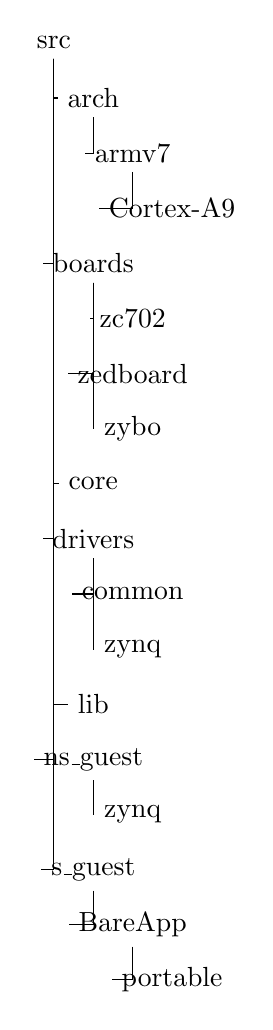
\begin{tikzpicture}[%
    grow via three points={one child at (0.5,-0.7) and %
    two children at (0.5,-0.7) and (0.5,-1.4)},%
    edge from parent path={(\tikzparentnode.south)%
    |- (\tikzchildnode.west)}]
  \node {src}
      child { node {arch}
        child {node {armv7}
        child {node {Cortex-A9}}}}
      child [missing] {}
      child [missing] {}
      child { node {boards}
        child {node {zc702}}
        child {node {zedboard}}
        child {node {zybo}}}
      child [missing] {}
      child [missing] {}
      child [missing] {}
      child { node {core}}
      child {node {drivers}
        child { node {common}}
        child {node {zynq}}}
      child [missing] {}
      child [missing] {}
      child {node {lib}}
      child {node {ns\_guest}
        child {node {zynq}}}
      child [missing] {}
      child { node {s\_guest}
        child {node {BareApp}
          child {node {portable}}}};
  \end{tikzpicture}
  \caption{Struktura direktorija izvršnog koda LTZVisora}
  \label{srcdir}
\end{figure}

Direktorij \textit{boards} sadrži skriptu za memorijsko povezivanje i kod koji je specifičan za određenu platformu te služi
podešavanju sigurnosti uređaja (npr. \gls{ttc}, \gls{uart}, globalno brojilo), SLCR registra (podešavanje sigurnosti memorijskih
segmenata, sigurnosti \gls{dma}, \textit{Etherneta}, \gls{ocm}...) i upravljačke programe uređaja koji se koriste (\gls{ttc} i \gls{uart}). Isto tako,
sadrži i inicijalizaciju \gls{gic}-a. Slijedeći direktorij, \textit{core}, sadrži jezgru LTZVisora koja je zadužena za postavljanje
početnog konteksta \textit{Nesigurnog} gosta i predavanje kontrole \textit{Sigurnom} gostu. \textit{drivers} direktorij sadrži upravljački
program \gls{gic}-a, a \textit{lib}, funkcije za rukovanje znakovnim nizovima i pristup registrima. Slika \textit{Nesigurnog} gosta se gradi
odvojeno od \textit{Sigurnog} gosta i LTZVisora, koji se izgrađuju zajedno, te direktorij \textit{ns\_guest} sadrži kod za uključivanje
slike \textit{Nesigurnog} gosta u sliku cjelokupnog sustava i atribute potrebne za pokretanje \textit{Nesigurnog} gosta. Zadnji,
\textit{s\_guest}, direktorij sadrži kod \textit{Sigurnog} gosta i tablicu prekidnih vektora \textit{Sigurnog} gosta.

\chapter{Operacijski sustav Linux}
Linux je operacijski sustav otvorenog koda te je prvenstveno namijenjen stolnim računalima (spada u \gls{gpos}).
Otvorenost koda omogućila je prilagođenje Linuxa za ugradbena računala.
Rastom mogućnosti procesora za ugradbena računala, sve je veća i potražnja za operacijskim sustavom Linux za ugradbena
računala. Linux je obično tražen zbog već gotove podrške za sučelja koja su potrebna u aplikaciji koja se razvija, npr.
mrežna podrška. Važne komponente Linuxa su jezgra, datotečni podsustav i \textit{Device Tree} koji su opisani u nastavku
ovog poglavlja. Kod ugradbenih računala, datotečni podsustav i jezgra operacijskog sustava su komprimirani.
Kako bi se Linux mogao pokrenuti, nužno je imati program pokretač (npr. U-Boot) koji će pripremiti platformu za izvođenje
Linuxa. Priprema platforme sastoji se od:
\begin{itemize}
  \item{inicijalizacije memorijskog sustava i periferija}
  \item{učitavanja slike Linuxa u \gls{ram} memoriju}
  \item{predaje ulaznih argumenata Linuxu}
  \item{pripremanja serijske konzole za jezgru (ovaj korak je izborni, ako se postave odgovarajući parametri za automatsko
  pokretanje jezgre OS-a)}
  \item{predaje kontrole jezgri OS-a.}
\end{itemize}
Neposredno prije nego što program pokretač skoči na početnu instrukciju jezgre Linuxa, pokretač
pripremi tri parametra koja su nužna za pokretanje Linuxa. Parametri se prenose preko registara opće namjene R0-R2, gdje
R0 mora sadržavati 0, R1 tip platforme (jedinstveni identifikator platforme) i R2 početnu adresu \textit{Device Tree} binarne
datoteke.

\section{Komponente operacijskog sustava Linux}
Kao što je već spomenuto, Linux za ugradbena računala sadrži tri glavne komponente sustava: datotečni podsustav, \textit{Device
Tree} i jezgru operacijskog sustava. Svaka od tih komponenata može biti izgrađena raznim alatima, u ovom radu je izabran
Xilinxov alat \textit{PetaLinux} koji ima mogućnost izgradnje svih komponenata odjednom. Svaka od komponenata je detaljnije
opisana u nastavku.

\subsection{\textit{Device Tree}}
\textit{Device Tree} je podatkovna struktura koja opisuje konfiguraciju hardvera kojeg će Linux koristiti. Sadrži sve potrebne
informacije o procesorima u sustavu, veličini memorije i konfiguraciji prekida i periferija. Struktura se upisuje u datoteku
ekstenzije \textit{.dts} ili \textit{.dtsi}, gdje je \textit{.dts} konačna datoteka koja može uključivati dodatne informacije
sadržane u \textit{.dtsi} datotekama \cite{xlnx}. Ako datoteke \textit{.dts} i \textit{.dtsi} sadrže informacije o istim komponentama,
u konačnici se uzima podatak iz \textit{.dts} datoteke. \textit{Device Tree} je važan jer opisuje hardver na način koji je
razumljiv Linuxu, a uz to, omogućuje Linuxu da nema fiksnu konfiguraciju hardvera \cite{plnx}. Svaki upravitelj uređajima ili modul
u \textit{Device Tree} strukturi je opisan čvorom koji sadrži sve postavke uređaja. Obzirom na vrstu upravitelja, upravitelj
može imati čvorove djece i čvor roditelja. Korjenski čvor je roditelj svim ostalim čvorovima te se sastoji od:
\begin{itemize}
  \item{čvora koji sadrži informacije o procesorima platforme}
  \item{čvor koji sadrži informacije o memoriji}
  \item{izborni čvor koji može sadržavati konfiguracijske podatke (parametre jezgre, lokaciju datotečnog podsustava...)}
  \item{čvor koji označava istoznačnice (alijase)}
  \item{čvorove koji sadrže informacije sabirnica platforme.}
\end{itemize}
Sintaksa \textit{Device Tree} strukture prikazana je slikom \ref{devtree_sintax}.

\begin{figure}[H]
  \centering
  \lstset{xleftmargin=.1\textwidth}
  \begin{lstlisting}
    node@address{
      property_name = "property_value";
      byte_property_name = [hex1 hex2 hex3 hex4];
      child_node@address{
        reference = <&reference_node>;
      };
    };
  \end{lstlisting}
  \caption{Sintaksa \textit{Device Tree} strukture}
  \label{devtree_sintax}
\end{figure}

Binarni ekvivalent, potreban za konačnu sliku sustava, \textit{.dts} datoteke je \textit{.dtb} koja se dobije \gls{dtc} (engl.
\textit{Device Tree Compiler}) alatom.

\subsection{Datotečni podsustav}
Linux je operacijski sustav koji sve upravljačke programe uređaja drži u obliku datoteka, stoga je potrebno imati datotečni
podsustav (korjenski datotečni podsustav), kako bi Linux ispravno funkcionirao. Datotečna struktura odgovara strukturi
datotečnog sustava Linuxa za stolna računala, ali uz znatno manje elemenata koji se mogu i dodatno smanjiti pomoću alata
za izgradnju datotečnog podsustava (npr. \textit{BusyBox} kojeg koristi \textit{PetaLinux}). Datotečni podsustav je obično
pohranjen u stalnu memoriju, ali postoji mogućnost i za pohranu u \gls{ram} memoriju.
Postoje različiti tipovi datotečnih podsustava, a ovo su neki od njih:
\begin{itemize}
  \item{\textit{initramfs} - datotečni podsustav koji ima mogućnost pisanja u datotečni podsustav, ali promjene nisu stalne,
  tj. gube se nakon gubitka napajanja. Izvorno mjesto ovakvog datotečnog podsustava je \gls{ram}.}
  \item{\textit{initrd} - datotečni sustav koji je prethodio \textit{initramfsu} i vrlo sličnih mogućnosti. Također se nalazi
  u \gls{ram}-u.}
  \item{\textit{jffs2} - montira se u \textit{flash} memoriju, gdje se jedna particija \textit{flasha} obavezno mora zvati
  \textit{jffs2} te se treba pobrinuti da particija ima dovoljno memorije za datotečni podsustav.}
  \item{\gls{nfs} (engl. \textit{Network File System}) - datotečni sustav se montira preko mreže te ciljana platforma i sustav
  domaćin dijele isti datotečni podsustav.}
  \item{SD datotečni podsustav - sustav koji je posebno izgrađen za SD karticu.}
\end{itemize}
Novije verzije jezgre podržavaju komprimirane \textit{cpio} arhive te je iz tog razloga moguće ručno ispuniti datotečni
podsustav sa željenim sadržajem uz pomoć \textit{cpio} alata na Linuxu. Takve arhive se komprimiraju za Linux algoritmom
koji se može izabrati u izborniku alata kojim je datotečni podsustav građen.
Sadržaj datotečnog podsustava se najčešće odnosi na:
\begin{itemize}
  \item{sustavske biblioteke}
  \item{aplikacije}
  \item{alate i različite usluge (komandni sustav, \textit{web} pretraživači...)}
\end{itemize}

\newpage
\subsection{Jezgra}
Izgradnja jezgre se sastoji od izgradnje dva sustava:
\begin{itemize}
  \item{sustav koji je neovisan o arhitekturi za koju se jezgra gradi (raspoređivač procesa, sučelje sustavskih poziva,
  upravljački programi koji su neovisni o arhitekturi i mrežni podsustav)}
  \item{sustav koji se tiče hardvera platforme za koju se jezgra gradi (inicijalizacija platforme, uređaji vezani uz odabranu
  platformu, itd.)}
\end{itemize}
Jezgra se poziva pomoću programa pokretača koji skače na prvu instrukciju jezgre operacijskog sustava te prvo što jezgra radi je
provjera ulaznih argumenata. Ako su ulazni argumenti valjani, jezgra počinje izvršavati početni program koji se odnosi na
dekomprimiranje jezgre. Nakon što je dekomprimiranje gotovo, kreće se na inicijalizaciju sustava. Sekvenca inicijalizacije
koju izvršava jezgra:
\begin{enumerate}
  \item{Onemogućavaju se \gls{irq} i \gls{fiq}, inicijalizira se \textit{tick} sustava, memorijski sustav, podsustavi ovisni o arhitekturi,
  uz koje se u obzir uzimaju ulazni argumenti koje je predao program pokretač,}
  \item{Konfigurira se stog i raspoređivač zadataka,}
  \item{Alociraju se stranice i podešavaju određena memorijska područja,}
  \item{Podešavaju se prekidi, iznimke i \gls{gic},}
  \item{Brojilo korišteno kao \textit{tick} se podešava i omogućuju se prekidi te se izvodi dodatna inicijalizacija memorije i
  kalibriranje takta jezgre,}
  \item{Podešava se datotečni podsustav i inicijaliziraju se procesi, izvršavaju se \textit{daemon} programi koji su zaduženi
  za stvaranje niti (engl. \textit{thread}) jezgre,}
  \item{Jezgra se otključava i raspoređivač se pokreće,}
  \item{Inicijaliziraju se razni uređaji i mreža.}
\end{enumerate}
Važno je napomenuti da prije predaje kontrole jezgri operacijskog sustava, \gls{mmu} i podatkovna \textit{cache} memorija moraju biti
onemogućeni te početno stanje jezgre mora biti u \textit{supervisor} načinu rada uz \gls{irq} i \gls{fiq} maskirane (onemogućene). Ako
jezgra nije primila valjane ulazne argumente, izvršavanje koda jezgre se prekida uz serijski ispis odgovarajuće poruke.

\section{\textit{PetaLinux}}
\textit{PetaLinux} je skup alata koji olakšavaju izgradnju slike Linuxa. Sadržava \gls{dtc} alat za prevođenje \textit{Device Tree}
strukture, za izgradnju datotečnog podsustava koristi \textit{BusyBox} te jezgru Xilinxovog Linuxa preuzima s \textit{GitHuba}.
\textit{PetaLinux} ima više verzija koje su dostupne za instalaciju, a u ovom radu se je koristio \textit{PetaLinux} 2019.1 koji
koristi verziju Linuxa 4.19. Pomoću \textit{PetaLinux} sučelja moguće je konfigurirati jezgru preko izbornika koji se poziva
naredbom \textit{petalinux-config -c kernel}. Iz sučelja je moguće dodati ili ukloniti razne upravljačke programe uređaja,
module ili mogućnosti jezgre. Kako \textit{PetaLinux} koristi Xilinxov Linux, izbornik sadrži mogućnosti dodavanja raznih
upravljačkih programa napisanih posebno za Xilinxove platforme, kao što je to ZedBoard. Za konfiguriranje datotečnog podsustava,
koristi se poseban izbornik koji se pokreće naredbom \textit{petalinux-config -c rootfs} koji također ima mogućnost uklanjanja
i dodavanja raznih komponenti datotečnog podsustava te ima i mogućnost dodavanja korisničkih aplikacija u datotečni  podsustav.
\textit{Device Tree} Linuxa se konfigurira pomoću datoteke koja je predviđena za dodavanje korisničkih informacija koje se tiču
hardvera. Opće postavke cjelokupne slike sustava mogu se postaviti pomoću općenitog izbornika koji se poziva naredbom
\textit{petalinux-config}. Početni sadržaj ovog izbornika je prikazan slikom \ref{peta_menu}.
\begin{figure}[H]
  \centering
	\includegraphics[width=300pt]{peta_menu.png}%
	\caption{Izbornik \textit{petalinux-config} naredbe}
	\label{peta_menu}%
\end{figure}
Pomoću prikazanog izbornika
moguće je odabrati razne općenite postavke slika koje se generiraju naredbom \textit{petalinux-build}. Najvažnije postavke
se odnose na početnu adresu na kojoj će se nalaziti slika jezgre u memoriji i cjelokupna memorija koja je dostupna Linuxu.
Uz to, ovim izbornikom je moguće odabrati željenu vrstu datotečnog podsustava (gdje su ponuđene vrste koje su navedene u
prethodnim poglavljima). Navedenim izbornikom se mogu upravljati i nekim postavkama \textit{Device Tree} strukture. Velik dio
postavki se odnosi na upute U-Bootu kako pronaći i pokrenuti jezgru operacijskog sustava. Vrlo korisni dio za početnike je
izbor \textit{Help} koji daje detaljniji opis ponuđenih komponenti te daje upute nesigurnom korisniku može li ukloniti
određene komponente iz Linuxa. Još jedna korisna postavka koju nudi \textit{PetaLinux} je mogućnost stavljanja eksternog
izvora Linuxovog koda što je posebno važno kod aplikacija koje zahtijevaju izmjenu izvornog koda jezgre.\\
Uz instalacijski paket \textit{PetaLinuxa}, preuzmu se i razni predlošci koji olakšavaju stvaranje inicijalnog
\textit{PetaLinux} projekta za odgovarajuću platformu s inicijalnim postavkama koje su valjane za odabranu platformu. Nakon
izgradnje sustava, slika jezgre Linuxa za Zynq-7000 platforme je naziva \textit{zImage} koja je komprimirana. Ako se
za datotečni podsustav odabere \textit{initramfs}, komprimirana slika datotečnog podsustava je automatski sadržana u
\textit{zImage} slici. Binarni oblik \textit{Device Tree} strukture je generiran u datoteku naziva \textit{system.dtb}.

\section{Prilagođenje Linuxa kao \textit{Nesigurnog} gosta LTZVisora}
Preporuka ARM-a je da složeniji operacijski sustavi budu namijenjeni \textit{Nesigurnom} svijetu, jer je kod sustava s većom
količinom koda veća vjerojatnost pronalaženja prolaza do probijanja sigurnosti. Zbog tog razloga, autori LTZVisora također
preporučuju implementaciju \gls{gpos}-a kao \textit{Nesigurnog} gosta. Prilagođenje kompleksnog sustava kao što je to Linux za \textit{Nesigurni}
svijet \textit{TrustZone} platforme je posao koji zahtjeva vrlo dobro poznavanje arhitekture jezgre operacijskog sustava, kao
i detaljno poznavanje platforme za koju se Linux prilagođava. Pristup prilagođenju može biti sljedeći: ako se Linux priprema
za \textit{Nesigurni} svijet, ključno je omogućiti konfiguriranje jezgre koje zahtjeva pristup \textit{Sigurnoj} memoriji, odnosno registrima
kojima može pristupiti samo \textit{Sigurni} svijet. Ovakav pristup, odmah u početku, uklanja potrebu za detaljnim poznavanjem
dijela jezgre operacijskog sustava koji je neovisan o arhitekturi platforme što znatno smanjuje vrijeme prilagodbe jezgre
\textit{Nesigurnom} svijetu. Uz takav pristup, jasno je i da se \textit{Device Tree} mora promijeniti. Prilagođenje Linuxa se sastoji
i od pripreme LTZVisora za Linux te su postupci prilagodbe dani u nastavku.

\subsection{Stvaranje cjelokupne slike Linuxa}
Arhitektura LTZVisora zahtjeva jednu izvršnu datoteku \textit{Nesigurnog} gosta, dok se Linux sastoji od više slika sustava (datotečnog
podsustava, \textit{Device Tree} strukture i jezgre). Uz to, Linux zahtjeva i program pokretač koji će pripremiti jezgru za
početak izvršavanja. Jasno je da je potrebno sve slike sustava Linux i program pokretač povezati u jednu izvršnu datoteku
koju će LTZVisor kasnije učitati u \gls{ram}. Jedan od intuitivnih načina na koji se to može postići je pomoću skripte za memorijsko
povezivanje u kojoj su naznačene adrese za svaku komponentu operacijskog sustava Linux. U ovom radu se je iskoristila mogućnost
koju nudi \textit{PetaLinux}, a tiče se vrste datotečnog podsustava. Kao datotečni podsustav odabrao se
\textit{initramfs} zbog mogućnosti da je takav datotečni podsustav odmah uključen u sliku jezgre Linuxa što doprinosi smanjenju
otiska cjelokupne slike Linuxa. Kada bi se koristio drugi datotečni podsustav, u skriptu za memorijsko povezivanje bilo bi
potrebno dodati poseban adresni prostor koji sadrži datotečni podsustav koji najvjerojatnije ne bi bio u potpunosti popunjen.
Sve što je potrebno u skripti za memorijsko povezivanje je adresa na kojoj se sprema \textit{Device Tree}, adresa minimalnog
koda koji predaje parametre jezgri Linuxa i adresu na kojoj se nalazi jezgra. Adrese na kojima su smještene komponente Linuxa
su prikazane tablicom \ref{adr_space}.

\begin{table}[H]
  \centering
  \begin{tabular}{ | p{3cm} | p{6cm} |}
    \hline
    \textbf{Adresa} & \textbf{Slika}\\
    \hline
    0x2000000 & \textit{Device Tree}\\
    \hline
    0x2007000 & Program pokretač\\
    \hline
    0x2008000 & Jezgra i datotečni podsustav  Linuxa\\
    \hline
  \end{tabular}
  \caption{Adresni prostor komponenata Linuxa}
  \label{adr_space}
\end{table}

Program pokretač se sastoji od jedne funkcije koja predaje potrebne parametre jezgri Linuxa i skače na početnu adresu jezgre.
Početna funkcija jezgre se može identificirati pomoću alata \textit{arm-none-eabi-objdump} koja ima mogućnost iz binarne
datoteke ispisati niz asemblerskih instrukcija ili simbola koje sadrži izvršna datoteka. Najjednostavnije je iskoristiti
navedeni alat za ispis tablice simbola sadržanih u izvršnoj datoteci. Ispisom simbola vidi se da se početna točka jezgre
Linuxa naziva \textit{\_binary\_images\_linux\_zImage\_start} koja se može iskoristiti kao funkcija s tri ulazna argumenta.
Ulazni argumenti su redom: R0, R1 i R2, gdje R0 sadrži 0, R1 jedinstveni identifikator ZedBoarda koji je 3378 i početna adresa
\textit{Device Tree} strukture koja je definirana u skripti za memorijsko povezivanje (0x2000000). Prije nego se sve slike
povežu u konačnu sliku, potrebno je konvertirati sliku jezgre i \textit{Device Tree} u binarne datoteke pomoću alata
\textit{arm-none-eabi-objcpy}. Nakon toga, slike se mogu povezati u jednu koja se može iskoristiti za LTZVisor.

\subsection{Izmjene operacijskog sustava Linux}
Kao što je već napomenuto, prilikom prilagođenja Linuxa za izvršavanje u \textit{Nesigurnom} svijetu treba voditi posebnu brigu o
pristupu Linuxa hardveru. Da bi uopće imalo smisla tražiti dijelove izvornog koda koji bi mogli biti problematični za
\textit{Nesigurni} svijet, jasno je da programer mora biti vrlo dobro upoznat arhitekturom \textit{TrustZone} ekstenzije, kao i
platforme za koju se Linux prilagođava. Iako to nije nužno, poželjno je da je programer upoznat s arhitekturom operacijskog
sustava kojeg prilagođava. Poznavanje arhitekture operacijskog sustava znatno olakšava lociranje nastalih problema, ali se
oni mogu otkriti i praćenjem toka programa od zadnjeg ispisa kojeg je dao Linux.

\subsubsection{Izmjene \textit{Device Tree} strukture}
Prije svega, \textit{Device Tree} mora biti ispravan. U \textit{Device Tree} strukturi se nalazi čvor koji sadrži informaciju
o memorijskim segmentima i njihovim veličinama koje Linux može koristiti. Navedeni čvor mora sadržavati ispravne informacije
o memoriji kako bi Linux mogao povezati fizičke i virtualne adrese bez generiranja pogreške. Opis memorijskog čvora korišten
u ovom projektu dan je slikom \ref{mem_node}. Polje čvora \textit{reg} opisuje lokaciju i veličinu \gls{ram}-a dodijeljenu Linuxu.

\begin{figure}[H]
  \lstset{xleftmargin=.1\textwidth}
  \begin{lstlisting}
    memory {
      device_type = "memory";
      reg = <0x00000000 0x1bdfffff>;
    };
  \end{lstlisting}
  \caption{Memorijski \textit{Device Tree} čvor}
  \label{mem_node}
\end{figure}

Kada bi memorijski čvor ostao kako \textit{PetaLinux} ima izvorno postavljeno (veličina memorijskog prostora od 0x2000000),
tada bi se pojavila pogreška prilikom rane inicijalizacije jezgre i izvođenje Linuxa bi bilo zaustavljeno.
Ostali čvorovi moraju sadržavati
točne informacije o uređajima koje Linux koristi te se u strukturi moraju nalaziti uređaji koje Linux koristi (primjer takvog
uređaja je globalno brojilo koje služi kao \textit{tick} OS-a). Uređaji koje Linux koristi, u \textit{Device Tree} strukturi moraju sadržavati informaciju da
je uređaj dostupan što se postiže dodavanjem \textit{status = "okay";} u čvor uređaja. Primjer ispravno konfiguriranog čvora
globalnog brojila prikazan je slikom \ref{glob_timer}.

\begin{figure}[H]
  \lstset{xleftmargin=.1\textwidth}
  \begin{lstlisting}
    global_timer: timer@f8f00200 {
      compatible = "arm,cortex-a9-global-timer";
      reg = <0xf8f00200 0x20>;
      interrupts = <1 11 0x301>;
      interrupt-parent = <&intc>;
      status = "okay";
      clocks = <&clkc 4>;
    };
  \end{lstlisting}
  \caption{Konfiguracijski čvor globalnog brojila}
  \label{glob_timer}
\end{figure}

Polje \textit{compatible} služi kao uputa Linuxu da pronađe odgovarajući
upravljački program za čvor. Slično kao kod memorijskog čvora, polje \textit{reg} opisuje baznu adresu globalnog brojila i
veličinu registarskog područja brojila. Svaki čvor mora sadržavati i informacije o prekidima te se one opisuju svojstvima
čvora \textit{interrupts} i \textit{interrupt-parent}. Tip prekida opisan je prvim poljem svojstva \textit{interrupts} (0 za
\gls{spi}, 1 za \gls{ppi}), drugo polje predstavlja prekidni broj i treće polje opisuje osjetljivost prekida i kojim procesorima je prekid
namijenjen. Upravitelj prekidom dan je \textit{interrupt-parent} svojstvom koji sadrži referencu na drugi čvor u \textit{Device
Tree} strukturi koji opisuje \gls{gic}. Opis izvora takta za uređaj, dan je \textit{clocks} svojstvom uređaja koji sadrži referencu
na signal takta koji je opisan u SLCR čvoru.
Kod generiranja \textit{Device Tree} strukture, \textit{PetaLinux} automatski opiše sve resurse platforme za koju se
\textit{Device Tree} generira. Poželjno je iz generirane \textit{Device Tree} strukture izbaciti sve resurse koji se koriste
kao sigurni uređaji (npr. \gls{ttc}0) ili barem postaviti njihovo stanje u \textit{status = "disabled";} koje onemogućava korištenje
resursa.

\subsubsection{Izmjene jezgre Linuxa}
Dobra početna točka kod izmjene jezgre je u direktoriju odgovarajuće arhitekture izvornog koda Linuxa. U slučaju ZedBoard
platforme, radi se o \textit{arch/arm/mach-zynq} direktoriju koji sadrži kod za inicijalizaciju platforme potrebnu za
pokretanje Linuxa. Ako se pogleda sadržaj navedenog direktorija, vidi se \textit{slcr.c} datoteka za koju je jasno da su
potrebne promjene (SLCR je dostupan samo \textit{Sigurnom} svijetu, a nužan je za npr. podešavanje signala takta za razne uređaje).
Funkcije za pristup SLCR registru, originalno su implementirane kako je prikazano slikom \ref{slcr_orig}.

\begin{figure}[H]
  \begin{lstlisting}
    static int zynq_slcr_write(u32 val, u32 offset)
    {
      return regmap_write(zynq_slcr_regmap, offset, val);
    }

    static int zynq_slcr_read(u32 *val, u32 offset)
    {
    	return regmap_read(zynq_slcr_regmap, offset, val);
    }
  \end{lstlisting}
  \caption{Pristup Linuxa SLCR-u}
  \label{slcr_orig}
\end{figure}

Funkcije \textit{regmap\_write} i \textit{regmap\_read} kao ulazni argument primaju virtualnu adresu koja je povezana s fizičkom
baznom adresom SLCR registra te se kasnije prevodi u fizičku adresu. Pozivanje ovih funkcija izaziva \textit{external abort}
zbog pristupanja \textit{Sigurnoj} memoriji. Kako bi se ove funkcije uspješno izvele, potrebno je implementirati funkcije za pristup
SLCR registru koji će biti izveden intervencijom LTZVisora. LTZVisor već implementira sustavske pozive koji se mogu iskoristiti
kao zahtjev \textit{Nesigurnog} gosta za čitanje i pisanje \textit{Sigurne} memorije. Izmijenjene funkcije za pristup SLCR-u prikazane su slikom \ref{slcr_secure}.

\begin{figure}[H]
  \lstset{breaklines=true}
  \begin{lstlisting}
    static int zynq_slcr_write(u32 val, u32 offset)
    {
      secure_write(val, zynq_slcr_base + offset);
      return 0;
    }

    static int zynq_slcr_read(u32 *val, u32 offset)
    {
    	*val = secure_read(zynq_slcr_base + offset);
    	return 0;
    }
  \end{lstlisting}
  \caption{Implementirane funkcije za pristup SLCR-u}
  \label{slcr_secure}
\end{figure}

Za razliku od izvornih funkcija implementiranih za pristup SLCR-u, funkcije \textit{secure\_write} i \textit{secure\_read} kao
ulazni argument primaju fizičku adresu registra kojem se pristupa. Varijabla \textit{zynq\_slcr\_base} je globalna, te Linux
prilikom inicijalizacije u nju spremi virtualnu adresu SLCR registra te je potrebno izmijeniti taj dio koda tako da se u
varijabli nalazi fizička adresa. Izmjenu je potrebno napraviti u istoj datoteci u funkciji za odgovarajuću inicijalizaciju.
Navedene funkcije su implementirane pomoću \gls{smc} instrukcije te predavanjem potrebnih parametara (adrese i vrijednosti) LTZVisoru.
U svakoj od funkcija sa slike \ref{slcr_secure} je dodana instrukcija \textit{return 0;} jer funkcije trebaju vratiti 0 za
uspješan pristup SLCR-u, a manje od 0 ako je pristup bio neuspješan te je ovdje pretpostavljeno da će pristup biti uspješan.
Za stvarnu informaciju o uspješnosti pristupa trebalo bi promijeniti implementaciju sustavskih poziva u LTZVisoru.
Uz pristup SLCR-u, Linux pristupa i jednom od koprocesorskih registara koji je zadužen za upravljanje snagom u koji se može
upisivati samo u \textit{Sigurnom} svijetu. Za uspješno konfiguriranje registra za upravljanje snagom također je implementirana posebna
funkcija koja pomoću \gls{smc} instrukcije od LTZVisora zahtjeva \textit{Siguran} upis u registar. ACTLR je također registar koji je dostupan
samo \textit{Sigurnom} svijetu, ali nema potrebe za implementacijom posebnog poziva LTZVisoru za upis u ACTLR jer su Linuxovi upisi u
registar zadovoljeni postavljanjem početnog konteksta \textit{Nesigurnog} gosta.
Uz promjene u izvornom kodu jezgre Linuxa, potrebno je i isključiti \gls{vfp} (engl. \textit{Vector Floating Point}) podršku da se
izbjegne \textit{undefined} iznimka na početku izvođenja \textit{init} skripte datotečnog podsustava. \gls{vfp} se može isključiti
pomoću izbornika koji se pokreće naredbom \textit{petalinux-config -c kernel}.\\
Navedene promjene su minimalne za uspješno pokretanje operacijskog sustava Linux kao \textit{Nesigurnog} gosta LTZVisora. Iako se Linux
uspješno pokreće nakon navedenih promjena, u ispisu kojeg Linux daje vide se neke dodatne pogreške koje se javljaju tokom
inicijalizacije. Pogreške se mogu vidjeti u isječku ispisa na slici \ref{plnx_errors}.

\begin{figure}[H]
  \centering
  \includegraphics[width=400pt]{error_output.png}
  \caption{Pogreške prilikom pokretanja Linuxa}
  \label{plnx_errors}
\end{figure}

Pogreška koja se odnosi na \gls{dmac} (\textit{\gls{dma} Controller}) se javlja zbog netočnog opisa \gls{dma} upravitelja u \textit{Device
Tree} strukturi. Naime, \textit{PetaLinux} prilikom generiranja \textit{Device Tree} strukture pretpostavlja \textit{Sigurno} stanje i
time automatski opisuje \gls{dmac} koji pripada \textit{Sigurnom} svijetu (Zynq-7000 platforme imaju poseban \gls{dmac} za \textit{Sigurni} i poseban za
\textit{Nesigurni} svijet čije se adrese razlikuju). Da se ukloni takva pogreška, potrebno je u \textit{Device Tree} umjesto \gls{dmac}
\textit{Sigurnog} svijeta, opisati \gls{dmac} \textit{Nesigurnog} svijeta (prvenstveno se odnosi na promjenu bazne adrese upravitelja).
Adresa \gls{dma} upravitelja \textit{Nesigurnog} svijeta je 0xf8004000.
Slijedeća pogreška koja se može pojaviti je vezana uz \gls{ocm} te se javlja u slučaju da je \textit{zynq\_slcr\_read} neispravno
implementiran (treba imati na umu da funkcija vraća pročitanu vrijednost preko ulaznog argumenta, a ne kao povratnu vrijednost
funkcije).

\subsection{Izmjene u LTZVisoru}
Uz izmjene Linuxa, potrebne su i izmjene u LTZVisoru koje se odnose na pripremu hardverskih resursa za korištenje u \textit{Nesigurnom}
svijetu i dodavanje sustavskog poziva za upis u koprocesorski registar za kontroliranje snage. Promjene koje su potrebne se
implementiraju u \textit{boards/zedboard} direktoriju izvornog koda LTZVisora. U \textit{board.c} datoteci se nalazi funkcija
zadužena za inicijalizaciju cjelokupnog \textit{TrustZone} sustava (podešavanje sigurnosti odgovarajućih uređaja i određivanje
koji memorijski segmenti pripadaju \textit{Sigurnom}, a koji \textit{Nesigurnom} svijetu). Navedena inicijalizacija platforme se odnosi na
konfiguriranje odgovarajućih SLCR registara. Funkcija zadužena za inicijalizaciju se zove \textit{board\_init} te minimalna
promjena u ovoj funkciji obuhvaća dopuštanje Linuxu da koristi globalno brojilo koje je nužno za uspješno pokretanje Linuxa.
Dopuštanje korištenja globalnog brojila sastoji se od upisa u dva registra SACR (engl. \textit{Secure Access Control Register})
i NSACR (engl. \textit{Non-Secure Access Control Register}) koji služe za konfiguraciju dozvole pristupa \textit{Nesigurnog} svijeta
privatnom i globalnom brojilu.\\
Dodatna promjena se odnosi na podešavanje \gls{dma} upravitelja, odnosno označavanje da će se \gls{dma} upravitelj koristiti u \textit{Nesigurnom}
svijetu. Prilikom podešavanja \gls{dma} upravitelja, nužno je da se \gls{dma} upravitelj drži u \textit{resetu}. Nakon što je \gls{dma} upravitelj
podešen, mora se pustiti iz \textit{reseta}. Opisane promjene prikazane su slikom \ref{tz_init}.
Kao što je prikazano, prije upisa u SLCR registre potrebno ga je prije svega otključati te po završetku pristupa zaključati.
Uz navedene promjene, potrebno je i označiti prekid globalnog brojila kao \gls{irq}, odnosno kao prekid \textit{Nesigurnog} svijeta
što se dodaje u \textit{ltzvisor\_hw.c} datoteku.

\begin{figure}[H]
  \lstset{breaklines=true, xleftmargin=.05\textwidth}
  \begin{lstlisting}
    uint32_t board_init(void){
      write32( (void *)SLCR_UNLOCK, SLCR_UNLOCK_KEY);
      ...
      write32( (void *)DMAC_RST_CTRL, 1);
      write32( (void *)TZ_DMA_NS, 0x1);
      write32( (void *)TZ_DMA_IRQ_NS, 0x0000ffff);
      write32( (void *)TZ_DMA_PERIPH_NS, 0xf);
      write32( (void *)DMAC_RST_CTRL, 0);
      ...
      write32( (void *)SCU_SAC, 0xf);
      write32( (void *)SCU_NSAC, 0xfff);
      ...
      write32( (void *)SLCR_LOCK, SLCR_LOCK_KEY);
    }
  \end{lstlisting}
  \caption{Funkcija inicijalizacije \textit{TrustZone} platforme}
  \label{tz_init}
\end{figure}

\chapter{Operacijski sustav za rad u stvarnom vremenu (\gls{rtos})}
\gls{rtos} ili operacijski sustav za rad u stvarnom vremenu je operacijski sustav namijenjen sustavima s vremenskim ograničenjima
te je čest odabir kod ugradbenih računala \cite{ppius}. Jezgra \gls{rtos}-a predstavlja minimalnu implementaciju operacijskog
sustava te uključuje:
\begin{itemize}
  \item {raspoređivač zadataka}
  \item{jezgrine objekte (zadatke, sinkronizacijske mehanizme, redove poruka...)}
  \item{usluge (vremenske, upravljanje resursima, prekidi).}
\end{itemize}
Operacijski sustavi koji spadaju u \gls{rtos} su QNX, VxWorks, Nucleus, FreeRTOS i drugi. Svima njima su zajedničke sljedeće
karakteristike:
\begin{itemize}
  \item {pouzdanost}
  \item{mali memorijski otisak u odnosu na \gls{gpos}}
  \item{odziv u stvarnom vremenu}
  \item{raspoređivanje zadataka prilagođeno za rad u stvarnom vremenu.}
\end{itemize}
\gls{rtos} ima prednost u tome što nema posebnih hardverskih zahtjeva (kao što to \gls{gpos} ima za npr. \gls{mmu} jedinicom) te ga je zbog toga
moguće prilagoditi na velik broj platforma, uključujući i mikrokontrolere. Sama jezgra operacijskog sustava je pogonjena jednim
brojilom koje je glavni okidač zamjene konteksta između zadataka. Prednost ovakvog operacijskog sustava u odnosu na
\textit{bare-metal} aplikacije je što postoji mogućnost istiskivanja zadataka. Ova karakteristika operacijskom sustavu
pruža mogućnost da prioritetniji zadaci obave potrebni posao prije od onih koji su nižeg prioriteta, što nije moguće kod
\textit{bare-metal} aplikacija.

\section{FreeRTOS}
FreeRTOS je operacijski sustav za rad u stvarnom vremenu otvorenog koda. Ovaj operacijski sustav je optimiran prema kriteriju
malih zahtjeva (memorijski zahtjevi i procesorska moć) te je prvenstveno namijenjen ugradbenim računalima \cite{osur}. Zbog
malih zahtjeva, pogodan je za implementaciju na mikrokontrolerima. Otvorenost koda FreeRTOS-a, omogućila je da se FreeRTOS
prilagodi za velik broj platformi, pa se tako može pronaći i FreeRTOS prilagođen za Xilinxov ZedBoard. Verzija FreeRTOS-a
korištenog u ovom projektu je v10.1.3 koja se može dobiti generiranjem \gls{bsp}-a \engl{Board Support Package} u Xilinx \gls{sdk}
2019.1. FreeRTOS koristi jedinstven način imenovanja varijabli i funkcija kojeg je zbog urednosti koda poželjno koristiti i
u razvoju FreeRTOS aplikacija. Na početku imena varijabli, dodaje se posebni identifikator koji govori kakvog tipa je
varijabla. Funkcije koriste slično imenovanje te njihov identifikator govori o tipu povratne vrijednosti. Identifikatori
varijabli mogu biti sljedeći:
\begin{itemize}
  \item{\textit{c} - \textit{char}}
  \item{\textit{s} - \textit{short}}
  \item{\textit{l} - \textit{long}}
  \item{\textit{u} - \textit{unsigned}}
  \item{\textit{p} - \textit{pointer}}
  \item{\textit{e} - \textit{enum}}
  \item{\textit{v} - \textit{void}}
  \item{\textit{x} - složeni tip varijable (struktura).}
\end{itemize}
Navedeni identifikatori se mogu i međusobno kombinirati. Funkcije mogu imati još jedan dodatan identifikator koji se ne koristi
kod varijabli, a to je \textit{prv} koji označava privatnu funkciju koja se koristi samo u \textit{.c} datoteci u kojoj je
definirana. Nadalje, u nazivu funkcije se nalazi i ime datoteke u kojoj je funkcija definirana, npr.
\textit{vTaskStartScheduler} je funkcija koja vraća \textit{void} vrijednost te je definirana u \textit{task.c} datoteci.
Prilikom prevođenja izvornog koda, FreeRTOS zahtjeva jednu datoteku u kojoj su upute za izgradnju jezgre operacijskog sustava.
Datoteka je naziva \textit{FreeRTOSConfig.h} te prilikom razvoja FreeRTOS aplikacija mora uvijek biti prisutna. U navedenoj
datoteci se nalaze razne definicije konstanti koje upućuju jezgru koje dijelove treba uključiti u jezgru ili koje dijelove
izbaciti iz jezgre. Konfiguriranje ove datoteke odgovara postupku konfiguriranja Linuxove jezgre, samo što konfiguriranje
jezgre Linuxa ima predviđeno sučelje za to (koje se pokreće naredbom \textit{petalinux-config}). FreeRTOS zadaci se često
implementiraju kao funkcije s beskonačnom petljom i koje dobrovoljno prepuštaju procesorsko vrijeme zadacima nižeg prioriteta
korištenjem zahtjeva za odgađanjem \engl{delay}.

\subsection{Programska podrška za Zynq-7000}
Programska podrška FreeRTOS-a se sastoji od malog broja datoteka koje u potpunosti implementiraju funkcionalnost \gls{rtos}-a.
U glavnom direktoriju izvornog koda FreeRTOS-a, dobivenog Xilinx \gls{sdk} alatom, se nalaze četiri datoteke koje su specifične
baš za ZedBoard. To su \textit{port\_asm\_vectors.S}, \textit{port.c}, \textit{portASM.S} i \textit{portZynq7000.c}. Ostale
platforme za koje je FreeRTOS prilagođen, također imaju vlastite \textit{port.c} i \textit{portASM.S} datoteke. Ostale
datoteke se mogu prenositi na druge platforme bez potrebe za ikakvim izmjenama.\\
Datoteka \textit{port\_asm\_vectors.S} sadrži tablicu prekidnih vektora te kod za konfiguraciju koprocesorskog registra koji
sadrži početnu adresu tablice prekidnih vektora. U \textit{port.c} se nalaze funkcije koje koriste podatke specifične za
hardver na kojem se FreeRTOS izvodi. Podaci se odnose na podatke specifične za upravitelja prekidima i upravljanje CPSR
registrom, kao i početnu inicijalizaciju konteksta zadatka (početni sadržaj stoga zadatka). Isto tako, datoteka sadrži i
funkcije za upravljanje prekidima koje se koriste za ostvarenje kritičnih sekcija. Obrada prekida u FreeRTOS-u je izvedena
tako da se u svakoj obradi provjerava ima li koji prioritetniji zadatak spreman za izvođenje od onog koji se je prekinuo te
ako ima, izvodi se zamjena konteksta i počinje se izvoditi prioritetniji zadatak. Navedena obrada je implementirana u
\textit{portASM.S} datoteci. Kako je FreeRTOS pogonjen brojilom čiji period označava jedan otkucaj \engl{tick}, većina
zamjene konteksta će se izvesti prilikom obrade prekida toga brojila. Prilikom obrade prekida, moguće je pozvati i dodatnu,
korisnički definiranu funkciju koja se poziva u \textit{vApplication\gls{irq}Handler} funkciji. Ova funkcija je izvorno definirana
u \textit{portZynq7000.c} datoteci. Funkcija koja obrađuje prekid otkucaja se naziva \textit{FreeRTOS\_Tick\_Handler} te
je zadužena za povećanje broja otkucaja i mora biti pozvana prilikom svake obrade prekida otkucaja. Navedena funkcija je
definirana u \textit{port.c} datoteci. Konfiguriranje brojila koji generira otkucaje se izvodi funkcijom
\textit{FreeRTOS\_SetupTickInterrupt} koja je definirana u \textit{portZynq7000.c} datoteci.\\
Zamjena konteksta koja je okinuta dobrovoljnim prepuštanjem procesorskog vremena drugom zadatku se izvodi pomoću
\textit{supervisor} iznimke koja se generira \textit{portYIELD} makroom definiranim u \textit{portmacro.h} datoteci.
Obrada iznimke se sastoji od spremanja konteksta trenutno izvođenog zadatka, odabirom zadatka koji će se izvoditi slijedeći
i obnovom konteksta zadatka čije izvođenje će započeti izlaskom iz obrade iznimke. Funkcija koja bira slijedeći zadatak
se zove \textit{vTaskSwitchContext} koja je definirana u \textit{task.c} datoteci i gotovo cijela funkcija je izvedena kao
kritična sekcija (nužno je da funkcija ne bude prekinjena). U svakom trenutku izvođenja FreeRTOS aplikacije mora biti aktivan
barem jedan zadatak te se stoga prilikom pokretanja raspoređivača zadataka stvara \textit{idle} zadatak koji se aktivira
kad više nema nijednog korisničkog zadatka spremnog za izvođenje. Funkcija \textit{idle} zadatka je implementirana u
\textit{port.c} datoteci, pod imenom \textit{portTASK\_FUNCTION}. Korisnička aplikacija koja se poziva u navedenoj funkciji
je \textit{vApplicationIdleHook} koja je početno definirana u \textit{portZynq7000.c} datoteci. Izvođenje korisničkih zadataka
na ZedBoard platformi odgovara izvođenju programa u sustavskom načinu rada.

\subsection{Prilagodba FreeRTOS-a kao \textit{Sigurnog} gosta LTZVisora}
FreeRTOS je izvorno implementiran kao operacijski sustav koji kao izvor prekida koristi \gls{irq}. Poznato je da dizajn LTZVisora
zahtjeva \gls{fiq} kao izvor prekida \textit{Sigurnog} svijeta te se prilagođenje \textit{Sigurnog} FreeRTOS-a odnosi na
prilagođenje jezgre da koristi \gls{fiq} umjesto \gls{irq}. Prvo što je potrebno promijeniti je funkciju koja se poziva prilikom pojave
\gls{fiq} prekida u tablici prekidnih vektora \textit{Sigurnog} svijeta. Kao funkciju za obradu \gls{fiq} prekida treba se postaviti
funkcija za obradu prekida u \textit{portASM.S} datoteci. Kako se u \textit{portASM.S} datoteci pretpostavlja obrada \gls{irq}
prekida, u obradi prekida postoji dio koda gdje se način rada procesora mijenja iz \textit{supervisor} u \gls{irq} način rada.
Navedeni dio koda je potrebno promijeniti tako da se način rada promijeni u \gls{fiq}. Kao što je već spomenuto,
\textit{vTaskSwitchContext} funkcija je većinom izvedena kao kritična sekcija te je potrebno implementirati promjene u
jezgri FreeRTOS-a koje će omogućiti takvu funkciju obzirom na \gls{fiq} prekide. Kritična sekcija se obično implementira
maskiranjem odgovarajućeg prekida, za \gls{fiq} to znači da je potrebno maskirati \gls{fiq} prekide u CPSR registru. Za Cortex-A procesore
postoji posebna oznaka koja govori o tome je li \gls{fiq} prekid moguće maskirati. Cortex-A9 sadrži navedeni podatak u NMFI
\engl{Nonmaskable \gls{fiq} Interrupt} bitu u SCTLR registru. Navedeni bit je predviđen samo za čitanje i ne može ga se
softverski konfigurirati te indicira na to da se \gls{fiq} ne može softverski maskirati. Poznato je da se \gls{fiq} automatski maskira
generiranjem \gls{fiq} prekida te se ta činjenica iskoristila za implementaciju kritične sekcije potrebne za
\textit{vTaskSwitchContext} funkciju.
\newpage
\noindent
Navedena funkcija se koristi u dva slučaja:
\begin{enumerate}
  \item {Kod obrade \gls{fiq} prekida}
  \item{Kod obrade \textit{supervisor} iznimke.}
\end{enumerate}
Jasno je da prvi slučaj zadovoljava potrebe implementacije kritične sekcije te je potrebno pobrinuti se za implementaciju
kritične sekcije drugog slučaja. Kako je već rečeno, ulazak u \textit{supervisor} iznimku se okida pozivom \textit{portYIELD}
makroa te je on izmijenjen tako da se umjesto \textit{supervisor} iznimke generira \gls{sgi} \gls{fiq} prekid. Nova implementacija
\textit{portYIELD} funkcije prikazana je slikom \ref{portyield}.
\begin{figure}[H]
  \begin{lstlisting}
  #define portYIELD()                               \
              interrupt_IPI_generate(8,1);          \
              __asm volatile( "dsb\n"               \
                              "isb")
  \end{lstlisting}
  \caption{Implementacija \textit{portYIELD} funkcije}
  \label{portyield}
\end{figure}
Poziv funkcije \textit{interrupt\_IPI\_generate(8,1);} generira \gls{sgi} prekidnog broja 8, za \gls{cpu}0 sučelje. U funkciji za
obradu prekida u \textit{portASM.S} datoteci se treba dodati dio koji će obraditi navedeni \gls{sgi}. Nakon što se u navedenoj
funkciji pročita prekidni broj generiranog prekida, potrebno je dodati kod prikazan slikom \ref{sgi}.
\begin{figure}[H]
  \lstset{breaklines=true, xleftmargin=.05\textwidth}
  \begin{lstlisting}
    CMP		r0, #8
    BNE		1f
    LDR 	r4, ulICCEOIRConst
    LDR		r4, [r4]
    STR		r0, [r4]
    POP		{r0-r4, r12}
    CPS		#FIQ_MODE
    POP		{LR}
    MSR		SPSR_cxsf, LR
    POP		{LR}
    B		FreeRTOS_SWI_Handler
  \end{lstlisting}
  \caption{Obrada \gls{sgi} prekida}
  \label{sgi}
\end{figure}
Labela \textit{1} odgovara kodu koji se izvorno nalazi nakon čitanja prekidnog broja \gls{fiq}-a. Dio koda prikazanog
slikom \ref{sgi} služi za obnovu konteksta u prekidu i poziv funkcije koja je služila za obradu \textit{supervisor} iznimke.
Na kraju, nužna promjena za ispravan rad FreeRTOS-a je postavljanje inicijalnog SPSR-a zadataka koji mora biti u obliku u
kojem su \gls{irq} prekidi maskirani. Navedeno se postiže izmjenom \textit{portINITIAL\_SPSR} varijable definirane u \textit{port.c}
datoteci.
Dodatna promjena koja se je implementira tiče se brojila za otkucaje. Izvorno, FreeRTOS za Zedboard koristi privatno brojilo
za otkucaje, a u ovom radu se koristi \gls{ttc}0. Da bi se \gls{ttc}0 mogao koristiti kao brojilo otkucaja, potrebno je izmijeniti
\textit{FreeRTOS\_SetupTickInterrupt} i \textit{FreeRTOS\_ClearTickInterrupt} koje konfiguriraju \gls{ttc}0 kao brojilo otkucaja,
odnosno brišu aktivno stanje prekida nakon obrade \gls{ttc}0 prekida. Kod implementacije \textit{FreeRTOS\_SetupTickInterrupt}
važno je imati na umu da prioritet brojila otkucaja mora biti najmanji mogući.
Uz navedene promjene u \textit{Sigurnom} FreeRTOS-u, zamjena konteksta LTZVisora se morala modificirati na način da se
\gls{fiq} ne obrađuje u nadglednom načinu rada, nego u \textit{Sigurnom} gostu te se kontekst \textit{Sigurnog} gosta dodatno
proširio.

\chapter{LTZVisor za višejezgrene procesore}
Predstavljeni dizajn LTZVisora ima jedan nedostatak, a to je situacija u kojoj \textit{Sigurni} gost ne prepušta procesorsko
vrijeme \textit{Nesigurnom} gostu \cite{amp_ltzvisor}. Takav slučaj je moguć kod aplikacija koje u \textit{Sigurnom} gostu
implementiraju zadatke koji predstavljaju veliko opterećenje procesora, što vodi izgladnjivanju procesora od strane
\textit{Sigurnog} gosta. Navedeni problem je glavna motivacija za proširenje LTZVisora za višejezgrene procesore. U nastavku su
opisani postupci prilagođenja LTZVisora za dva modela višejezgrenih konfiguracija, \gls{amp} i \gls{smp}. \gls{amp} inačica LTZVisora je razvijena
kada i originalna verzija LTZVisora, a \gls{smp} inačica je implementirana u sklopu ovog rada.

\section{Prilagođenje LTZVisora za \gls{amp}}
Kao što je već bilo prikazano, razvoj \textit{TrustZone} aplikacija se sastoji od razvoja:
\begin{itemize}
  \item {\textit{Sigurnog} softvera}
  \item{\textit{Nesigurnog} softvera}
  \item{softvera nadglednog načina rada procesora.}
\end{itemize}
Razvoj \textit{Sigurnog} i \textit{Nesigurnog} softvera podsjeća na razvoj \gls{amp} aplikacije: svaki svijet ima svoju posebnu
skriptu za memorijsko povezivanje i skriptu za pokretanje sustava. Isto tako, svaki svijet može implementirati svoj operacijski
sustav što se može i povezati s \gls{amp} konfiguracijom gdje svaka jezgra u sustavu implementira svoj operacijski sustav. Kod
usporedbe ovakva dva sustava, naziru se dvije značajne razlike:
\begin{enumerate}
  \item {Razvoj \textit{TrustZone} softvera pruža izolaciju između dva svijeta (dva operacijska sustava), dok običan razvoj
  \gls{amp} aplikacije to ne pruža.}
  \item{Kod običnih \gls{amp} aplikacija, operacijski sustavi imaju vlastitu jezgru dodijeljenu samo njima, dok kod
  \textit{TrustZone} aplikacija \textit{Sigurni} i \textit{Nesigurni} svijet dijele jednu jezgru.}
\end{enumerate}
\gls{amp} LTZVisor objedinjuje razvoj obične \gls{amp} aplikacije i razvoj \textit{TrustZone} softvera te time poboljšava performanse
originalnog LTZVisora.

\subsection{Arhitektura \gls{amp} LTZVisora}
\gls{amp} LTZVisor u potpunosti uklanja mogućnost pojave izgladnjivanja procesora od strane \textit{Sigurnog} softvera. Jedna jezgra
u sustavu izvodi softver \textit{Sigurnog} svijeta, odnosno zadužena je za izvođenje privilegiranog softvera. Druga jezgra
izvodi softver \textit{Nesigurnog} svijeta, odnosno zadužena je za izvođenje neprivilegiranog softvera. Pravilo na kojem je
temeljen model je da jedna jezgra implementira jedan svijet u jednom sigurnosnom stanju. Arhitektura \gls{amp} LTZVisora može se
vidjeti na slici \ref{amp_ltzvisor}.
\begin{figure}[H]
  \centering
  \includegraphics[width=300pt]{amp_ltzvisor}
  \caption{Arhitektura \gls{amp} LTZVisora \cite{amp_ltzvisor}}
  \label{amp_ltzvisor}
\end{figure}
Na slici se mogu vidjeti tri osnovne komponente:
\begin{itemize}
  \item {\textit{Nesigurni} gost čija se jezgra operacijskog sustava izvršava u \textit{supervisor} načinu rada, a aplikacije
  \textit{Nesigurnog} gosta u korisničkom načinu rada procesora \textit{Nesigurnog} svijeta}
  \item{\textit{Sigurni} gost čija se jezgra operacijskog sustava izvršava u \textit{supervisor} načinu rada, a aplikacije
  \textit{Sigurnog} gosta u korisničkom načinu rada procesora \textit{Sigurnog} svijeta}
  \item{LTZVisor koji se izvršava u najprivilegiranijem načinu rada procesora: nadglednom načinu rada.}
\end{itemize}
\newpage
\noindent
Zbog \gls{amp} modela, LTZVisor je podijeljen na dva dijela:
\begin{itemize}
  \item {jezgru LTZVisora}
  \item{sloj usluga \engl{Service Layer}.}
\end{itemize}
Jezgra LTZVisora je zadužena za sve ključne zadatke kao što su to konfiguriranje memorije, dodjeljivanje prekida i uređaja
svakom gost virtualnom stroju uz pružanje podrške za komunikaciju između procesora, odnosno gost virtualnih strojeva.
Sloj usluga je minimalna implementacija nadglednog načina rada procesora koji je zadužen za obradu i prosljeđivanje iznimaka,
kao i kontrolu nad komunikacijom između procesora. Iako se oba gosta izvode u privilegiranom načinu rada (\textit{supervisor}),
\textit{Sigurni} svijet ostaje u potpunosti izoliran od privilegiranog softvera \textit{Nesigurnog} svijeta. Dakle,
\textit{Nesigurni} softver ne može pristupiti niti mijenjati resurse koji su dodijeljeni \textit{Sigurnom} gostu. Svaki pristup
\textit{Nesigurnog} gosta \textit{Sigurnom} generira iznimku sloju usluga koji je zadužen za prosljeđivanje iznimke jezgri
LTZVisora.\\
Na početku izvođenja, LTZVisor svakom gostu dodijeli jednu jezgru, odnosno \gls{cpu}. Za \gls{gpos} je odabran Linux te je njemu
zbog jednostavnosti dodijeljen \gls{cpu}0 (Linux je izvorno namijenjen primarnoj jezgri procesora). Svaki OS ima \gls{mmu} i L1
\textit{cache} memoriju dodijeljene odgovarajućim jezgrama. L2 \textit{cache} memorija je dijeljena između procesora, ali zbog
arhitekture \textit{TrustZone} ekstenzije, postoji \textit{Sigurna} i \textit{Nesigurna} L2 \textit{cache} memorije te zbog
toga nije potrebno voditi brigu o koherenciji (koherencija je automatski očuvana hardverom). Uređajima direktno upravljaju gost
particije te su na početku statički dodijeljeni \textit{Sigurnom} ili \textit{Nesigurnom} svijetu da bi se očuvala izolacija
na razini uređaja. \gls{amp} LTZVisor prati prekidni model originalnog LTZVisora, gdje se \gls{fiq} dodjeljuje \textit{Sigurnom} gostu,
a \gls{irq} \textit{Nesigurnom} gostu. Inicijalizacija \gls{gic} distributera se izvodi \gls{cpu}1 jezgrom. Sloj usluga je zadužen za
inicijalizaciju odgovarajućeg \gls{cpu} sučelja. Obrada prekida je rješena tako da ako se \gls{fiq} pojavi na \gls{cpu}0, sloj usluga je zadužen
za prosljeđivanje prekida \gls{cpu}1 procesoru. Ako \gls{irq} dođe prilikom izvođenja \gls{rtos}-a u \textit{Sigurnom} svijetu, prekid se neće proslijediti
\gls{cpu}0. Praćenje vremena gost virtualnih strojeva omogućeno je dodjeljivanjem \gls{ttc}0 brojila \textit{Sigurnom} gostu i globalnog
brojila \textit{Nesigurnom} gostu.

\section{Prilagođenje LTZVisora za \gls{smp}}
Kao što je već opisano u prethodnim poglavljima, \gls{smp} može predstavljati veliko poboljšanje cjelokupne procesorske efikasnosti.
Iako je to za većinu slučajeva točno, postoji i određeni tip aplikacija kojima \gls{smp} nije dobar izbor. Primjer jedne takve
aplikacije je aplikacija koja u svakom trenutku izvršava samo jedan proces s jednom niti što znači da je uvijek samo jedan procesor aktivan.
Aplikacije koje imaju koristi od \gls{smp} konfiguracije su one koje implementiraju npr. određene vrste obrade signala koje
zahtijevaju veliku procesorsku moć. Ovo poglavlje predstavlja \gls{smp} LTZVisor koji se može iskoristiti kod potrebe za navedenim
tipom aplikacija te predstavlja sasvim novu inačicu LTZVisora čija je implementacija bila u planu od trenutka kada je LTZVisor
razvijen.

\subsection{Arhitektura \gls{smp} LTZVisora}
Model \gls{smp} LTZVisora prati jedan od predloženih ARM-ovih modela za razvoj \gls{smp} \textit{TrustZone} aplikacije. Navedeni model se
odnosi na konfiguraciju gdje \textit{Nesigurni} softver iskorištava \gls{smp} mogućnosti, dok se \textit{Sigurni} softver izvodi na
jednoj jezgri u sustavu. Kod ovakvog modela, u odnosu na originalni LTZVisor, nema potrebe za dodatnim promjenama
\textit{Sigurnog} softvera te se prilagođenje razvija promjenama u nadglednom načinu rada i u \textit{Nesigurnom} gostu.
Arhitektura \gls{smp} LTZVisora prikazana je slikom \ref{smp_ltzvisor}.
\begin{figure}[H]
  \centering
  \includegraphics[width=300pt]{smp_ltzvisor_arch}
  \caption{Arhitektura \gls{smp} LTZVisora}
  \label{smp_ltzvisor}
\end{figure}
Na slici se vide tri glavne komponente: \textit{Sigurni} gost (\gls{rtos}) koji se izvodi na \gls{cpu}0, \textit{Nesigurni} gost (\gls{gpos})
koji se izvodi kao \gls{smp} gost i LTZVisor koji se izvodi na obje jezgre platforme u \gls{smp} konfiguraciji.
Pokretanje cjelokupnog sustava započinje ulaskom \textit{Sigurnog supervisor} načina rada procesora u inicijalizacijski proces.
Početna inicijalizacija \textit{Sigurnog} softvera odnosi se na konfiguriranje SCR, NSACR, SCTLR i ACTLR te \gls{mmu},
\textit{cachea}, polja za predviđanje grananja i inicijalizacija \textit{Sigurnog} stoga i stoga nadglednog načina rada
procesora. Nakon toga, LTZVisor \gls{cpu}0 jezgre preuzima kontrolu te inicijalizira memoriju, \gls{gic} upravitelja prekidima te
dodjeljuje uređaje gost virtualnim strojevima. Uz to, \gls{cpu}0 LTZVisor pripremi sustav za izvođenje \textit{Sigurnog} i
\textit{Nesigurnog} softvera. Svi nabrojeni koraci su zajednički \gls{smp} LTZVisoru i originalnom LTZVisoru. Nakon što se izvrši
početna inicijalizacija, \gls{cpu}0 se na trenutak zaustavlja i predaje se kontrola \gls{cpu}1 LTZVisoru. Zaustavljanje \gls{cpu}0 je izvedeno
pomoću jednostavne implementacije koja je slična binarnom semaforu te ima istu namjenu kao i binarni semafor, a to je
sinkronizacijski mehanizam. Kad je \gls{cpu}0 zaustavljen, \gls{cpu}1 LTZVisor obavi početnu inicijalizaciju \gls{cpu}1 procesora i pripremi
\textit{Nesigurnog} gosta za izvođenje na \gls{cpu}1. Po završetku pripreme \gls{cpu}1 sustava, LTZVisor ponovno stavlja \gls{cpu}1 u \gls{wfe} stanje
te se iz njega budi na zahtjev \textit{Nesigurnog} gosta.

\subsubsection{Prekidni podsustav}
Prekidni podsustav prati predložen ARM-ov model kod implementacije \textit{TrustZone} aplikacija, a to je korištenje \gls{fiq}-a za
\textit{Sigurni} svijet i \gls{irq}-a za \textit{Nesigurni} svijet. Kao i kod prethodnih verzija LTZVisora,
osigurano je da \textit{Sigurni} gost ne propusti nijedan prekid na jezgri na kojoj se izvodi (\gls{cpu}0). Obrada prekida \gls{smp}
LTZVisora se odvija po sljedećem modelu:
\begin{enumerate}
  \item{Za \gls{cpu}0:}
    \begin{itemize}
      \item{ako se \gls{fiq} pojavi kad se izvodi \textit{Sigurni} gost, \textit{Sigurni} gost odmah obrađuje \gls{fiq} bez intervencije
      LTZVisora}
      \item{ako se \gls{fiq} pojavi za vrijeme izvođenja \textit{Nesigurnog} gosta, kontrolu preuzima LTZVisor koji radi zamjenu
      konteksta i pokreće \textit{Sigurni} gost koji odmah po početku izvođenja obrađuje \gls{fiq}}
      \item{ako se \gls{irq} pojavi za vrijeme izvođenja \textit{Sigurnog} gosta i ako je \gls{irq} namijenjen isključivo \gls{cpu}0, prekid će
      se obraditi tek po početku izvođenja \textit{Nesigurnog} gosta}
      \item{ako se \gls{irq} pojavi za vrijeme izvođenja \textit{Nesigurnog} gosta, \gls{irq} je obrađen prema standardnom modelu obrade
      prekida.}
    \end{itemize}
  \item{Za \gls{cpu}1:}
    \begin{itemize}
      \item{ako se pojavi \gls{fiq}, \gls{fiq} ostaje neobrađen}
      \item{\gls{irq} prekidi namijenjeni \gls{cpu}1 ili oba \gls{cpu}-a su obrađeni prema standardnom modelu obrade prekida.}
    \end{itemize}
\end{enumerate}
Pogledom na prekidni model \gls{smp} LTZVisora može se odmah uočiti jedna mana ovakvog modela, a to je da \gls{fiq} koji se pojavi na \gls{cpu}1
ostaje neobrađen, što u svakom slučaju nije poželjno. Ovakav model zahtjeva opreznu implementaciju \textit{Sigurnog} softvera
što se tiče prekidnog podsustava (prekidi moraju biti konfigurirani da se prosljeđuju samo \gls{cpu} sučelju na kojem se izvodi
\textit{Sigurni} softver). Ovaj problem se može riješiti i na elegantniji način, npr. prilikom pojave \gls{fiq}-a na \gls{cpu}1, LTZVisor
može rekonfigurirati prekid tako da se prekid prosljeđuje samo ispravnom \gls{cpu} sučelju ili samo javiti poruku o grešci
\textit{Sigurnom} gostu i prepustiti odluku o prekidu \textit{Sigurnom} gostu. LTZVisor je zadužen za konfiguraciju prekida
i dodjeljivanje uređaja gost virtualnim strojevima za oba \gls{cpu} sučelja. Uređaji su statički dodijeljeni virtualnim strojevima
kao i u prethodnim verzijama LTZVisora. Prilikom implementacije \gls{smp} rješenja, vodila se briga
o tome da \gls{gic} distributer bude inicijaliziran samo jednom te to izvodi LTZVisor na \gls{cpu}0 procesoru, dok su \gls{cpu} sučelja
inicijalizirana na svakom \gls{cpu}-u zasebno. Za praćenje stvarnog vremena virtualnih strojeva, \textit{Sigurnom} gostu je
dodijeljen \gls{ttc}0, a \textit{Nesigurnom} gostu je dodijeljeno globalno brojilo.

\subsubsection{Memorijski podsustav}
\textit{Sigurni} gost je implementiran kao \textit{bare-metal} aplikacija kojoj LTZVisor dodjeljuje 64~MB, dok
\textit{Nesigurni} gost implementira \gls{smp} Linux operacijski sustav te mu je dodijeljena preostala memorija koja iznosi 448~MB.
\textit{Sigurni} gost, zbog očuvanja jednostavnosti i predvidljivosti implementacije, ne koristi \gls{mmu} ni L1 ni L2 \textit{cache}
memorije. Uz to, ne koriste se ni polja za predviđanje grananja. Poznato je da Linux zahtjeva korištenje \gls{mmu} jedinice za
ispravno funkcioniranje te se podrazumijeva da će se \textit{Nesigurne} \gls{mmu} tablice za prevođenje koristiti. Isto tako, Linux
spada u sustave opće namjene te je nepredvidljivost do neke razine dozvoljena. Stoga, Linux koristi i L1 i L2 \textit{cache} te
polja za predviđanje grananja. Ključna činjenica koja omogućava ovakvu konfiguraciju gost virtualnih strojeva je da
LTZVisor ima pristup \textit{Nesigurnim} tablicama te je zbog toga moguće izvesti skok na virtualnu adresu
\textit{Nesigurnog} gosta.

\subsubsection{Komunikacijski model}
Za \gls{smp} LTZVisor, razvijena je jednostavna jednosmjerna komunikacija. Implementirani model omogućava slanje poruka od
\textit{Nesigurnog} gosta prema \textit{Sigurnom}. Komunikacija je razvijena kao aplikacija koja se pokreće pomoću Linuxove
ljuske. Pomoću aplikacije, željeni podatak se može upisati na određenu memorijsku lokaciju koja je označena kao
\textit{Nesigurna}. Nakon što je podatak upisan na danu adresu, Linuxova aplikacija pomoću sustavskog poziva generira
\gls{smc} poziv LTZVisoru s odgovarajućim identifikatorom koji signalizira da \textit{Nesgiurni} gost želi predati poruku
\textit{Sigurnom} gostu. LTZVisor dalje signalizira \textit{Sigurnom} gostu da postoji nepročitani podatak na odgovarajućoj
lokaciji pomoću \gls{sgi} prekida. \textit{Sigurni} gost interpretira poruku \textit{Nesigurnog} gosta u obradi \gls{sgi} prekida.
Ovisno o tome s kojeg procesora se poruka šalje, LTZVisor generira \gls{sgi} s različitim prekidnim brojevima.

\subsection{Promjene u nadglednom načinu rada procesora}
Prvo što je potrebno kod razvoja \gls{smp} aplikacija je početna adresa aplikacije koja će se izvoditi na sekundarnom procesoru.
U \gls{smp} LTZVisor implementaciji, početna adresa za \gls{cpu}1 je definirana u skripti za memorijsko povezivanje. Da bi varijabla u
skripti za memorijsko povezivanje sadržavala ispravnu adresu, potrebno je kod za početnu inicijalizaciju \gls{cpu}1 procesora staviti
u posebnu sekciju. Sljedeće što je potrebno je kod koji će se izvršavati po pokretanju \gls{cpu}1 sustava. Početni kod sadrži
inicijalizaciju koja je vrlo slična inicijalizaciji koja se izvršava na \gls{cpu}0. Razlika je u tome što nema potrebe za
inicijalizacijom stoga \textit{Sigurnog} gosta te sadrži samo inicijalizaciju stoga nadglednog načina rada. Nadalje, da se
sustav pripremi za izvršavanje \textit{Nesigurnog} gosta, inicijaliziraju se i SCR i NSACR registri s jednakim vrijednostima
kao i kod \gls{cpu}0. Nakon što su početna adresa za \gls{cpu}1 i inicijalizacijski kod definirani, LTZVisor je spreman za buđenje \gls{cpu}1
procesora. Buđenje \gls{cpu}1 je izvedeno u asembleru te je prikazano slikom \ref{wake_cpu1}.
\begin{figure}[H]
  \centering
  % \lstset{language=[x86masm]Assembler}
  \lstset{numbers=left, numbersep=2pt, numberstyle=\tiny, breaklines=true, xleftmargin=.2\textwidth}
  \begin{lstlisting}[firstnumber=1]
    _wake_cpu1:
      ldr r0,=0xfffffff0
      ldr r1,=_cpu1_entry_address
      str r1,[r0]
      dmb
      sev
      bl wait_till_cpu1_boots
      b ltzvisor_kickoff
  \end{lstlisting}
  \caption{Postupak buđenja \gls{cpu}1}
  \label{wake_cpu1}
\end{figure}
Simbol \textit{\_cpu1\_entry\_address} sadrži početnu adresu za \gls{cpu}1 koja se upisuje na odgovarajuću adresu koju \gls{cpu}1 čita
odmah po buđenju. Instrukcija \textit{dmb} se koristi da se osigura završetak pisanja u memoriju. Buđenje se okida pozivom
instrukcije \textit{sev} te su nakon izvršavanja te instrukcije, oba procesora platforme aktivna. Kako bi se osigurala ispravna
inicijalizacija \gls{cpu}1 sustava, \gls{cpu}0 se blokira skokom na funkciju \textit{wait\_till\_cpu1\_boots} koja u petlji čeka da se
postavi zastavica koju postavlja \gls{cpu}1 točno prije nego se \gls{cpu}1 ponovno stavi u \gls{wfe} stanje. Kad je za \gls{cpu}0 sigurno da krene
s daljnjim izvođenjem, skače se na \textit{ltzvisor\_kickoff} funkciju iz koje se poziva \textit{Sigurni} gost te iz navedene
funkcije nema povratka.\\
\gls{wfe} stanje \gls{cpu}1 procesora je isto kao i početno \gls{wfe} stanje u kojem se \gls{cpu}1 nalazi prije pokretanja LTZVisora na njemu.
Nakon što je LTZVisor završio s inicijalizacijom, na adresu 0xFFFFFFF0 se upisuje 0 te \gls{cpu}1 čeka događaj sustava i
vrijednost različitu od 0 na navedenoj adresi. Opisani postupak implementiran je kodom prikazanim slikom \ref{cpu1_wfe}.
\begin{figure}[H]
  \centering
  \lstset{numbers=left, numbersep=2pt, numberstyle=\tiny, breaklines=true, xleftmargin=.2\textwidth}
  \begin{lstlisting}[firstnumber=1]
    put_cpu1_back_to_sleep:
      ldr r0, =0xfffffff0
      ldr r1, =0
      str r1, [r0]
      bl unlock_cpu0
      dsb
      isb
    wait:
      wfe
      ldr r0, =0xfffffff0
      ldr r1, [r0]
      cmp r1, #0
      beq wait
      movs pc, r1
  \end{lstlisting}
  \caption{Postavljanje sekundarnog procesora u \gls{wfe} stanje}
  \label{cpu1_wfe}
\end{figure}
Funkcija \textit{unlock\_cpu0} postavlja potrebnu zastavicu koja će osloboditi \gls{cpu}0, čime započinje izvođenje \textit{Sigurnog}
gosta. Ako se \gls{cpu}1 probudi iz \gls{wfe} stanja i na odgovarajućoj adresi pročita vrijednost 0, procesor se ponovno stavlja u \gls{wfe}
stanje. Kad je vrijednost različita od 0, LTZVisor predaje kontrolu \textit{Nesigurnom} gostu skokom na adresu koja je upisana
na 0xFFFFFFF0 lokaciji. To se izvodi instrukcijom \textit{movs pc, r1} koja, uz skok na odgovarajuću adresu, učita
vrijednost iz SPSR u CPSR. Kako Linux zahtjeva da se procesori pokreću u \textit{supervisor} načinu rada, u SPSR-u se mora
nalaziti ispravna vrijednost te se ta vrijednost postavlja prilikom postavljanja početnog konteksta \textit{Nesigurnog} gosta.
Kao što je napomenuto, LTZVisor je zadužen za inicijalizaciju upravitelja prekidima te inicijalizira \gls{cpu} sučelje za svaki
procesor posebno. Kako se LTZVisor koristi kao \textit{domaćin} \gls{smp} \textit{Nesigurnog} gosta, važno je da se odgovarajući
\gls{sgi} prekidi označe kao \textit{Nesigurni}. \gls{sgi} se koriste za sinkronizaciju između jezgra u sustavu te su nužni za ispravno
funkcioniranje \gls{smp} Linuxa. Linux prati preporuke ARM-a za \textit{Nesigurni} svijet te koristi \gls{sgi} s prekidnim brojevima: ID0~-~ID7. Navedeni prekidi
se obavezno moraju naznačiti da će se koristiti za \textit{Nesigurni} svijet. Poznato je da svaki procesor implementira
vlastiti set \gls{sgi} prekida te je zbog toga nužno označiti odgovarajuće prekide kao \textit{Nesigurne} na obje jezgre. Kako je
već navedeno, Linux koristi globalno brojilo kao \textit{tick} operacijskog sustava te je važno napomenuti da globalno brojilo
pripada \gls{ppi} prekidima što znači da se i globalno brojilo mora označiti kao \textit{Nesigurno} na obje jezgre.\\
Zadnje što je potrebno promijeniti za uspješno pokretanje \gls{smp} Linuxa je omogućavanje korištenja \gls{vfp} podrške u
\textit{Nesigurnom} svijetu. Omogućavanje se sastoji od konfiguriranja dva registra: CPACR i FPEXC \engl{Floating Point
Exception Register}. FPEXC omogućava korištenje \gls{fpu} \engl{Floating Point Unit}, a CPACR omogućava korištenje \gls{fpu} koprocesorskih
registara u \textit{Nesigurnom} svijetu. Koprocesor CPACR je na \gls{cpu}0 izvorno podešen tako da dozvoljava \textit{Nesigurno}
korištenje \gls{fpu} koprocesorskih registara te ne \gls{cpu}0 nije potrebno dodatno konfigurirati navedeni koprocesorski registar. Za \gls{cpu}1
je izvorno onemogućeno pristupanje \gls{fpu} koprocesorskim registrima od strane \textit{Nesigurnog} svijeta te se na \gls{cpu}1, CPACR
mora konfigurirati.

\subsubsection{Komunikacijski model}
Dodatne promjene LTZVisora su bile potrebne kako bi bilo moguće implementirati komunikaciju između virtualnih strojeva.
Kako je već napomenuto, ovisno o tome s kojeg \gls{cpu}-a dolazi poruka, LTZVisor generira \gls{sgi} različitih prekidnih brojeva.
Tako se \gls{sgi} s prekidnim brojem 9 koristi za signaliziranje \textit{Sigurnom} gostu da poruka dolazi s \gls{cpu}0
\textit{Nesigurnog} gosta, dok se prekidni broj 10 koristi za signaliziranje \gls{cpu}1 \textit{Nesigurne} poruke. Kako Linux
koristi \textit{cache}, moguće je da se na odgovarajućoj lokaciji neće nalaziti najnoviji podatak (potrebni podatak će se
nalaziti u \textit{cache} memoriji) te je potrebno isprazniti \textit{cache} memoriju. Rukovanje \textit{cache} memorijom
u korisničkim aplikacijama Linuxa je nepraktično te je navedeno potrebno izvesti pomoću sustavskog poziva jezgri Linuxa.
Iz tog razloga rukovanje \textit{cacheom} se obavlja u LTZVisoru koji ima mogućnost pristupa \textit{Sigurnom} i
\textit{Nesigurnom cacheu}. Opisano prosljeđivanje \gls{cpu}0 poruke prikazano je slikom \ref{sgi_communicate}.

\begin{figure}[H]
  \lstset{numbers=left, numbersep=2pt, numberstyle=\tiny, breaklines=true, xleftmargin=.2\textwidth}
  \begin{lstlisting}
    communicate:
      push {r0-r12,lr}
      bl flush_icache_and_dcache
      bl cachel2_invalidate
      bl cachel2_clean
      pop {r0-r12,lr}
      push {r0-r2,lr}
      mov r0, #9
      mov r1, #1
      bl interrupt_IPI_generate
      pop {r0-r2,lr}
      movs pc, lr
  \end{lstlisting}
  \caption{Prosljeđivanje \textit{Nesigurne} poruke \textit{Sigurnom} gostu}
  \label{sgi_communicate}
\end{figure}

Ovime su napravljene sve potrebne izmjene u nadglednom načinu rada za uspješnu uspostavu komunikacije između virtualnih
strojeva. U nastavku su dane i promjene napravljene u \textit{Sigurnom} gostu.\\
Promjene u \textit{Sigurnom} gostu
obuhvaćaju dodatne funkcije koje služe za obradu \gls{sgi} prekida generiranih dolaskom \textit{Nesigurne} poruke. Za
demonstraciju ispravnog funkcioniranja komunikacije, odabrala se aplikacija koja preko \textit{Nesigurnog} gosta upravlja
LED diodama platforme čija stanja se mijenjaju u \textit{Sigurnom} softveru. ZedBoard sveukupno sadrži 8 LED dioda te
razvijena aplikacija ima mogućnost upravljanja svakom LED diodom posebno. \textit{Sigurni} softver u prekidnoj rutini
osvježava vrijednost koja će se sljedeća koristiti kao novo stanje LED dioda. Ako poruka dolazi s \gls{cpu}0 \textit{Nesigurnog}
gosta, ponašanje LED dioda ovisno o poslanoj vrijednosti je sljedeće:
\begin{itemize}
  \item{poslana vrijednost: 0x0 - sve LED diode će biti ugašene}
  \item{poslana vrijednost: 0xf - sve LED diode će biti upaljene}
  \item{poslana vrijednost: između 0x0 i 0x9 - LED dioda čiji redni broj na platformi odgovara poslanoj vrijednosti će biti
  upaljena}
  \item{sve ostalo će izazvati početno ponašanje LED dioda (\textit{blinky}).}
\end{itemize}
Ako poruka dolazi s \gls{cpu}1 \textit{Nesigurnog} gosta, ponašanje će biti isto kao i kad poruka dolazi s \gls{cpu}0 za sve slučajeve
osim za vrijednosti u itervalu od 0x1 do 0x8. Za navedenu iznimku ponašanje je obrnuto: odgovarajuća LED dioda će biti
ugašena, dok će sve ostale svijetliti.

\subsection{Promjene u \gls{smp} Linux \textit{Nesigurnom} gostu}
Promjene u \gls{smp} Linuxu su minimalne te se većina prilagodbe izvodi u LTZVisoru. Iako su promjene minimalne, potrebno je detaljno
poznavanje načina na koji se sekundarni procesor budi i uz to, potrebno je u Linuxu raspoznati gdje se i na koji način izvodi
buđenje sekundarnog procesora. Prije svega, potrebno je definirati nužne komponente u \textit{Device Tree} strukturi. Kod
verzije Linuxa koja se gradi za jednu jezgru, dovoljno je u procesorski čvor \textit{Device Tree} strukture staviti opis
samo one jezgre na kojoj će se Linux izvršavati. Kod \gls{smp} verzije je nužno opisati sve procesore koji će se koristiti za
implementaciju \gls{smp} Linuxa. Postavka u \textit{Device Tree} strukturi na koju treba posebno paziti se odnosi na konfiguriranje
prekida za globalno brojilo za koje je nužno da se označi da je prekid namijenjen jednom i drugom procesoru.\\
Promjene u jezgri Linuxa se implementiraju u \textit{arch/arm/mach-zynq/platsmp.c} datoteci. Prva funkcija koja se poziva
kod pokretanja sekundarnog procesora se zove \textit{zynq\_boot\_secondary} u kojoj se prvo provjerava status sekundarnog
procesora. Status se čita u \textit{eFuse} registru koji je dostupan samo u \textit{Sigurnom} svijetu te je potrebno
osigurati čitanje iz tog registra. Čitanje je ostvareno već implementiranom funkcijom \textit{secure\_read}. Kad se čitanje
iz tog registra ne bi osiguralo, Linux ne bi mogao doći do dijela programa gdje se priprema početna adresa za sekundarni
procesor. Isto tako, treba se osigurati predaja fizičke adrese potrebnog registra \textit{secure\_read} funkciji. Navedeni
dio koda se može slobodno zakomentirati, pošto je poznato da je sa sekundarnim procesorom sve u redu i da je spreman za
izvođenje. Iduća funkcija koja se poziva je \textit{zynq\_cpun\_start} koja pokreće sekundarni procesor. Funkcija kao ulazne
argumente prima početnu adresu i ID procesora za kojeg se početna adresa priprema. Ako se pogleda na koji način se poziva
navedena funkcija, vidi se da se kao prvi argument predaje \textit{\_\_pa\_symbol(\&secondary\_startup)}. Poznato je da Linux
koristi virtualne adrese te simbol \textit{\&secondary\_startup} predstavlja virtualnu adresu na kojoj se nalazi početni kod
za sekundarni procesor. Funkcija \textit{\_\_pa\_symbol} vraća fizičku adresu ulaznog argumenta što znači da je ulazni argument
\textit{zynq\_cpun\_start} funkcije točno ona adresa koju je potrebno upisati na 0xFFFFFFF0.\\
Postupak kojim Linux budi sekundarnu jezgru je sljedeći:
\begin{enumerate}
  \item{\gls{cpu}1 se stavlja u \textit{reset} i onemogućava mu se signal takta,}
  \item{Na adresu 0x00000000 se kopira minimalni kod koji služi za skok na \textit{\&secondary\_startup} adresu,}
  \item{Čisti se \textit{cache} memorija u memorijskom području koje obuhvaća kopirani kod s početnom adresom
  0x00000000 (nužno za očuvanje koherencije),}
  \item{\gls{cpu}1 se pušta iz \textit{reseta} i omogućava mu se signal takta nakon čega \gls{cpu}1 automatski skače na adresu
  0x00000000.}
\end{enumerate}
Ovakav postupak buđenja sekundarne jezgre je nedopustiv u implementaciji gdje se Linux koristi kao \textit{Nesigurni} gost
LTZVisora iz razloga što bi se izgubila inicijalizacija sustava za \textit{Nesigurni} gost \gls{cpu}1 procesora. Navedeni postupak
je zamijenjen s onim koji odgovara modelu LTZVisora. Prije opisa postupka buđenja, treba napomenuti da se upis na
0xFFFFFFF0 lokaciju mora izvesti u \textit{Sigurnom} stanju procesora (lokacija je nedostupna \textit{Nesigurnom}
svijetu). Postupak kojim je izvedeno pokretanje sekundarne jezgre u \textit{Nesigurnom} gostu LTZVisora je:
\begin{enumerate}
  \item {Linux generira zahtjev LTZVisoru za upis odgovarajuće adrese na 0xFFFFFFF0 lokaciju,}
  \item{LTZVisor upisuje početnu adresu za \gls{cpu}1 na odgovarajuću lokaciju te se vraća kontrola \textit{Nesigurnom} gostu,}
  \item{Linux generira \textit{sev} instrukciju.}
\end{enumerate}
U ovom slučaju nema potrebe za rukovanjem \textit{cache} memorijom jer se upis na 0xFFFFFFF0 lokaciju izvodi
LTZVisorom koji ne koristi \textit{cache} memoriju. Kad bi LTZVisor koristio \textit{cache}, bilo bi potrebno očistiti
\textit{cache} memoriju prije vraćanja kontrole \textit{Nesigurnom} gostu. Nakon što su implementirane navedene promjene,
Linux je spreman za pokretanje kao \gls{smp} \textit{Nesigurni} gost. Potvrda o tome da je \gls{cpu}1 uspješno pokrenut se vidi u ispisu
prilikom pokretanja Linuxa. Isječak koji to opisuje prikazan je slikom \ref{smp_boot_secondary}.
\begin{figure}[H]
  \centering
  \includegraphics[width=300pt]{cpu1_online}
  \caption{Isječak ispisa pokretanja \gls{smp} Linuxa}
  \label{smp_boot_secondary}
\end{figure}
Kada bi pokretanje \gls{cpu}1 procesora bilo neuspješno, Linux bi to javio porukom: \textit{\gls{cpu}1: failed to come online}.
Dodatna provjera o uspješnosti pokretanja sekundarnog procesora se može izvesti nakon što se Linux pokrene do kraja.
Informacije o procesorima u sustavu se mogu dobiti naredbom \textit{cat /proc/cpuinfo} što daje ispis prikazan slikom
\ref{cpuinfo}.
\begin{figure}[H]
  \centering
  \includegraphics[width=300pt]{cpuinfo}
  \caption{Sadržaj \textit{/proc/cpuinfo} datoteke}
  \label{cpuinfo}
\end{figure}
Navedena datoteka sadrži informacije o mogućnostima dostupnim procesorima u sustavu. Potvrda o tome da su aktivna oba
procesora se može dobiti ispisom \textit{/sys/devices/system/cpu/online} datoteke čiji je ispis prikazan slikom \ref{cpuonline}.
\begin{figure}[H]
  \centering
  \includegraphics[width=300pt]{cpuonline}
  \caption{Ispis \textit{/sys/devices/system/cpu/online} datoteke}
  \label{cpuonline}
\end{figure}
U ispisu su dani identifikacijski brojevi procesora koji označavaju procesore opisane u \textit{/proc/cpuinfo} datoteci.
Što se tiče frekvencija na kojima rade procesori, u ispisu na slici \ref{smp_boot_secondary} se vidi ukupna frekvencija
uzimajući u obzir oba procesora te iznosi oko 1333~MHz, dok se u ispisu \textit{/proc/cpuinfo} datoteke može vidjeti
frekvencija svakog procesora pojedinačno te ona iznosi približno 667~MHz.

\subsubsection{Komunikacijski model}
Za potrebe komunikacije između virtualnih strojeva, za Linux je razvijena korisnička aplikacija koja se poziva na zahtjev
korisnika putem Linuxove ljuske. Aplikacija prima dva ulazna argumenta, prvi označava fizičku adresu na koju se želi
pohraniti željeni podatak, a drugi argument predstavlja vrijednost koja se želi pohraniti. Kod razvoja ovakvog tipa aplikacija
za Linux, treba imati na umu da Linux radi s virtualnim adresama te je potrebno osigurati da se podatak upiše na ispravnu
fizičku lokaciju. Kako korisnik odabire željenu fizičku lokaciju, aplikacija se mora pobrinuti da izabranu fizičku lokaciju
poveže s virtualnom adresom. Navedeno je izvedeno pomoću \textit{mmap} funkcije koja zauzima određeno memorijsko područje u
kojem je sadržana željena fizička adresa. Memorijsko područje koje se zauzima \textit{mmap} funkcijom mora biti barem
veličine jedne stranice. Kolika je veličina jedne stranice koju koristi Linux, korisnik može saznati pomoću sustavskog
poziva \textit{sysconf} te se vrijednost dobivena navedenim sustavskim pozivom može koristiti za poziv \textit{mmap}
funkcije. Obzirom da se za odabranu fizičku adresu dobije jedno memorijsko područje određene veličine, odabrana fizička
lokacija se ne mora nalaziti na početku zauzetog memorijskog odjeljka. Iz tog se razloga potrebna virtualna memorija mora
izračunati tako da se podatak upiše na ispravnu fizičku lokaciju.\\
Odabrani model komunikacije zahtjeva da se nakon upisa podatka na odgovarajuću memorijsku lokaciju generira \gls{smc} instrukcija
kojom će LTZVisor biti obavješten o postojanju novih poruka za \textit{Sigurnog} gosta. Korisničke aplikacije Linuxa
se izvode u neprivilegiranom načinu rada procesora, odnosno u korisničkom načinu rada. Generiranje \gls{smc} instrukcije kada
se procesor nalazi u korisničkom načinu rada izaziva \textit{undefined} iznimku te je za potrebe generiranja \gls{smc}
instrukcije potrebno implementirati sustavski poziv. Sustavski poziv obrađuje jezgra operacijskog sustava koja se izvršava
u privilegiranom načinu rada te se zbog toga može iskoristiti za potrebe generiranja \gls{smc} instrukcije. Navedeni sustavski
poziv je definiran u \textit{arch/arm/kernel/sys\_arm.c} datoteci te je njegova implementacija prikazana slikom \ref{sendm}.

\begin{figure}[H]
  \lstset{numbers=left, numbersep=2pt, numberstyle=\tiny, breaklines=true, xleftmargin=.1\textwidth}
  \begin{lstlisting}[showstringspaces=false]
    asmlinkage long sys_sendm_to_secure(void)
    {
      asm volatile(".arch_extension sec\n"
                    "ldr r0, =0x9\n"
                    "smc #0\n");
      return 0;
    }
  \end{lstlisting}
  \caption{Definicija sustavskog poziva za slanje poruke \textit{Sigurnom} gostu}
  \label{sendm}
\end{figure}

Vrijednost 0x9 služi kao identifikator LTZVisoru po kojem LTZVisor prepoznaje koju akciju poduzeti za primljenu iznimku.
Deklaracija sustavskog poziva se mora nalaziti u \textit{include/linux/syscall.h} datoteci. Uz to, potrebno je definirati
i broj sustavskog poziva koji služi kao identifikacijski broj sustavskog poziva jezgri operacijskog sustava. To je moguće
dodavanjem linija prikazanih slikom \ref{sc_num} u \textit{include/uapi/asm-generic/unistd.h} datoteku.

\begin{figure}[H]
  \begin{lstlisting}
    #define __NR_sendm_to_secure 294
    __SYSCALL(__NR_sendm_to_secure, sys_sendm_to_secure)
  \end{lstlisting}
  \caption{Definicija broja novog sustavskog poziva}
  \label{sc_num}
\end{figure}

Prilikom dodavanja novog broja sustavskog poziva, treba voditi brigu o tome da se ukupni broj sustavskih poziva treba
osvježiti. To se izvodi redefiniranjem \textit{\_\_NR\_syscalls} konstante koja je definirana u
\textit{include/uapi/asm-generic/unistd.h} datoteci. Navedene promjene su dovoljne da je sustavski poziv dostupan jezgri
operacijskog sustava, no ovim promjenama implementirani sustavski poziv još uvijek nije dostupan korisničkoj aplikaciji.
Sustavski pozivi dostupni korisniku definiraju se u tablici sustavskih poziva koja se može pronaći u
\textit{arch/arm/tools/syscall.tbl}. Dodavanjem linije prikazane slikom \ref{user_sc}, sustavski poziv postaje dostupan
korisniku te ga je moguće pozvati sa \textit{syscall(400);}, gdje je 400 broj sustavskog poziva koji je rezerviran za
korisnika.

\begin{figure}[H]
  \begin{lstlisting}
    400 common  sendm_to_secure   sys_sendm_to_secure
  \end{lstlisting}
  \caption{Sustavski poziv dostupan korisniku}
  \label{user_sc}
\end{figure}

\chapter{Testiranje \gls{smp} LTZVisor rješenja}
Nad implementiranim rješenjem, provedena su mjerenja, odnosno testiranja vremena izvođenja nužnih dijelova koda LTZVisora.
Mjerenja su provedena pomoću očitanja stanja \gls{ttc}1 brojila u odgovarajućim trenucima. Rezultati mjerenja su početno u obliku
broja koji predstavlja broj otkucaja brojila na određenoj frekvenciji. \gls{ttc}1 brojilo se je podesilo da broji $1~ms$ od
početka odsječka kojeg se promatra te se na kraju odsječka zaustavilo. Vrijeme ekvivalentno broju otkucaja brojila se dobije
pomoću:
\begin{equation}
  \label{ttc_eq}
  T=\frac{N}{f}
\end{equation}
U (\ref{ttc_eq}), $T$ je vremenski period u kojem je brojilo bilo aktivno nakon zadnjeg postavljanja, $N$ broj otkucaja
i $f$ frekvencija na kojoj radi brojilo. Frekvencija na kojoj radi \gls{ttc}1 iznosi $27.75~MHz$. \textit{Sigurni} gost se je
podesio tako da se svakih $100~ms$ okida prekid. Jednaka mjerenja su se provela na modificiranoj verziji originalnog
LTZVisora i na \gls{smp} LTZVisor verziji s \gls{smp} Linux \textit{Nesigurnim}
gostom. Mjerenja koja su provedena su:
\begin{enumerate}
  \item{Obrada \gls{smc} iznimke: obrada se odnosi na \gls{smc} iznimke generirane od strane \textit{Nesigurnog} gosta prilikom
  inicijalizacije sustava. \gls{ttc}1 se postavlja i omogućava na ulasku u tablicu prekidnih vektora te se zaustavlja prije
  povratka u \textit{Nesigurni} gost (na kraju obrade).}
  \item{Spremanje konteksta \textit{Sigurnog} gosta: \gls{ttc}1 se postavlja i omogućava na ulasku u \gls{smc} iznimku rezerviranu
  za LTZVisorov raspoređivač zadataka te se zaustavlja po završetku spremanja \textit{Sigurnog} konteksta.}
  \item{Obnova konteksta \textit{Nesigurnog} gosta: \gls{ttc}1 se omogućava prije dohvaćanja adrese globalne varijable u kojoj
  se nalazi \textit{Nesigurni} kontekst i zaustavlja se po završetku obnove konteksta.}
  \item{Potvrda \gls{fiq}-a: \gls{ttc}1 se omogućava na ulasku u tablicu prekidnih vektora nadglednog načina rada (konkretno za
  \gls{fiq} prekid) i zaustavlja se nakon što se pročita vrijednost iz registra za potvrdu prekida u \gls{fiq} prekidnoj rutini.}
  \item{Spremanje konteksta \textit{Nesigurnog} gosta: \gls{ttc}1 se omogućava prije dohvaćanja adrese globalne varijable u kojoj
  je pohranjen kontekst \textit{Nesigurnog} gosta i zaustavlja se nakon što je kontekst spremljen u varijablu.}
  \item{\gls{fiq} obrada: \gls{ttc}1 se omogućava prije skoka u \textit{Sigurni} gost i zaustavlja se nakon upisa u registar za
  označavanje kraja obrade prekida.}
  \item{Obnova konteksta \textit{Sigurnog} gosta: \gls{ttc}1 se omogućava nakon spremanja konteksta \textit{Nesigurnog} gosta
  i zaustavlja nakon što se \textit{Sigurni} kontekst obnovi.}
  \item{Vrijeme od početka izvođenja \textit{Sigurnog} zadatka do ulaska u raspoređivač LTZVisora: \gls{ttc}1 se omogućava
  nakon poziva LTZVisorovog raspoređivača i zaustavlja se na ulasku u \gls{smc} obradu.}
\end{enumerate}
Testiranja su provedena na procesorima koji rade na $667~MHz$. Za svako mjerenje određena je maksimalna vrijednost
koja se je dobila mjerenjem za oba slučaja. Svako mjerenje se je ponovilo 10 puta te je od 10 slučajeva izabrana
maksimalna dobivena vrijednost. U svakom mjerenju se je prikupilo 400 uzoraka, osim za prvi slučaj u kojem se je u
obzir uzelo 200 uzoraka iz razloga što se prilikom inicijalizacije \textit{Nesigurnog} gosta \gls{smc} pozove oko 200 puta.
Rezultati su prikazani slikom \ref{max_perf}. Koordinatna
os $x$ sadrži brojeve koji odgovaraju rednim brojevima prethodno nabrojenih tipova mjerenja, a $y$ os sadrži vremensko
trajanje izvođenja određenog dijela koda u $\mu s$.

\begin{figure}[H]
  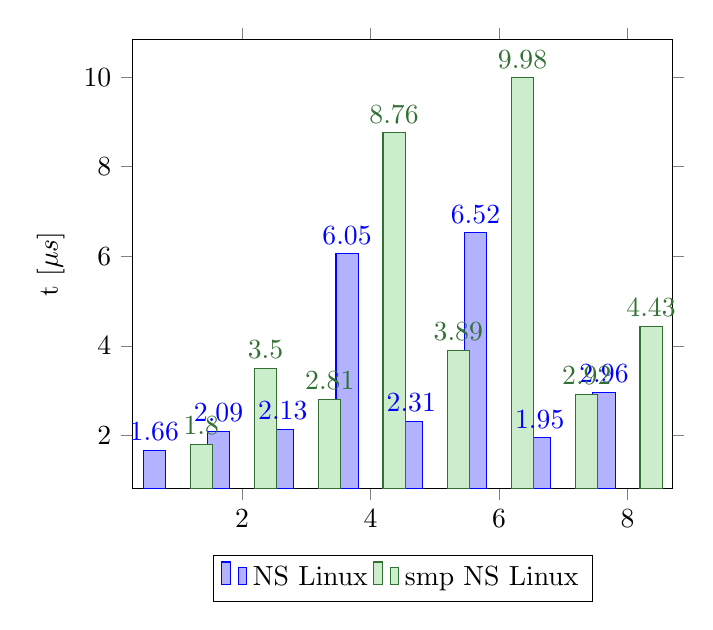
\begin{tikzpicture}
    \centering
    \begin{axis}[
    	x tick label style={
    		/pgf/number format/1000 sep=},
    	ylabel={t $[\mu s]$},
    	enlargelimits=0.1,
    	legend style={at={(0.5,-0.15)},
    	anchor=north,legend columns=-1},
      ymax=10,
    	ybar=9pt,
      bar width = 8pt,
      ytick align = outside,
      nodes near coords,
      x tick label style={rotate=0,anchor=north},
      y tick label style={rotate=0,anchor=east},
    ]
    \addplot
    	coordinates {(1,1.658) (2,2.090)
    		 (3,2.126) (4,6.054)
         (5,2.306) (6,6.523)
         (7,1.946) (8,2.955)};
    % [black!70!white,fill=black!20!white]
    \addplot[green!30!black!80!white, fill=green!65!black!20!white]
    	coordinates {(1,1.802) (2,3.495)
    		(3,2.811) (4,8.757)
        (5,3.892) (6,9.982)
        (7,2.919) (8,4.432)};
    \legend{NS Linux, \gls{smp} NS Linux}
    \end{axis}
  \end{tikzpicture}
  \caption{Maksimalno vrijeme izvođenja određenih odjeljaka \gls{smp} LTZVisora}
  \label{max_perf}
\end{figure}

Na slici se vidi kako su maksimalne vrijednosti trajanja odgovarajućih odsječaka koda \gls{smp} LTZVisora veće od vrijednosti
koje daje LTZVisor za jednu jezgru. Višestrukim ponavljanjem mjerenja utvrđeno je da se navedene maksimalne vrijednosti
\gls{smp} LTZVisora pojavljuju nakon pokretanja inicijalne skripte datotečnog podsustava \gls{smp} Linuxa. Navedeni dio inicijalizacije
je jedini dio u kojem se pojavljuju ovako visoke vrijednosti. Ovakvo ponašanje nije očekivano niti poželjno te treba ukloniti
razlog tome (još je nepoznat). Ovakvo ponašanje nije prisutno kod obrade \gls{smc} iznimke izazvane \textit{Nesigurnim} gostom
iz razloga što su svi zahtjevi generirani prije početka izvođenja inicijalne skripte datotečnog podsustava.
Ponavljanjem mjerenja, bilo je moguće uočiti i da se maksimalne vrijednosti svakog mjerenja međusobno razlikuju kod
\gls{smp} LTZVisor rješenja. Npr. kod mjerenja potrebnog za priznanje \gls{fiq} prekida, zabilježene maksimalne vrijednosti od 10
mjerenja su u rasponu od $7.532~\mu s$ do $8.757~\mu s$. Ovakav rezultat mjerenja ukazuje na određenu mjeru
nepredvidljivosti, koja bi mogla biti uzrokovana \textit{cacheom}, \gls{tlb}-ovima, predviđanjem grananja ili uranjenim
dohvatom \engl{prefetch} podataka i instrukcija. Svim ovim resursima je zajedničko da je, ako su resursi omogućeni, potrebna oprezna implementacija
kod korištenja više procesora u sustavu.
Kako su \textit{cache}, \gls{mmu} i predviđanje grananja isključeni u \textit{Sigurnom} gostu, izvor
problema bi mogao biti uranjeni dohvat. Uranjenim dohvatom se upravlja ACTLR registrom koji je zajednički
\textit{Nesigurnom} i \textit{Sigurnom} gostu te je moguće rješenje za uklanjanje navedenog problema dodavanje ACTLR
registra u kontekst virtualnih strojeva.
Ponavljanjem mjerenja za LTZVisor koji je implementiran za jednu jezgru, maksimalne vrijednosti su približno jednake,
što pokazuje da nepredvidljivost nije prisutna u navedenoj verziji LTZVisora.
Kako bi se pokazalo da se prikazane maksimalne vrijednosti pojavljuju rijetko, od
prikupljenih uzoraka se je izračunala srednja vrijednost te su navedeni rezultati prikazani slikom \ref{avg_perf}.

\begin{figure}[H]
  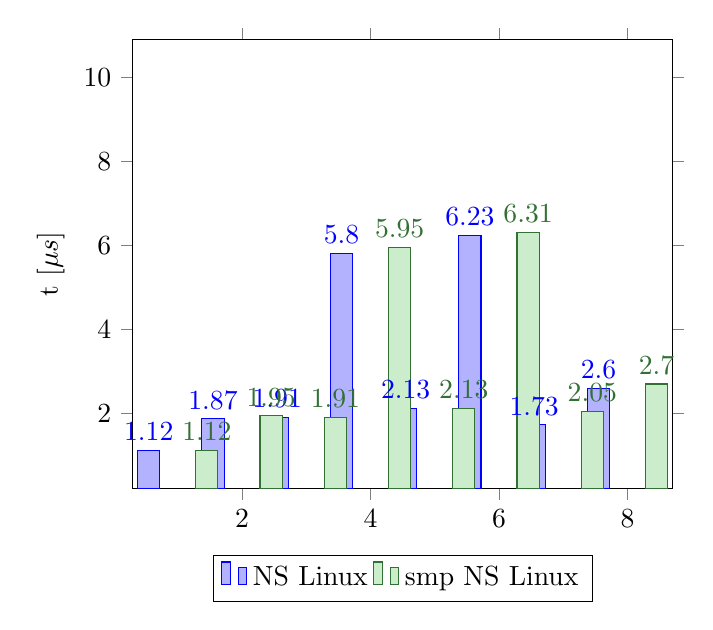
\begin{tikzpicture}
    \centering
    \begin{axis}[
    	x tick label style={
    		/pgf/number format/1000 sep=},
    	ylabel={t $[\mu s]$},
    	enlargelimits=0.1,
    	legend style={at={(0.5,-0.15)},
    	anchor=north,legend columns=-1},
      ymax=10,
    	ybar=13pt,
      bar width = 8pt,
      ytick align = outside,
      nodes near coords,
      x tick label style={rotate=0,anchor=north},
      y tick label style={rotate=0,anchor=east},
    ]
    \addplot
    	coordinates {(1,1.117) (2,1.874)
    		 (3,1.910) (4,5.802)
         (5,2.126) (6,6.234)
         (7,1.730) (8,2.595)};
    % [black!70!white,fill=black!20!white]
    \addplot[green!30!black!80!white, fill=green!65!black!20!white]
    	coordinates {(1,1.117) (2,1.946)
    		(3,1.910) (4,5.946)
        (5,2.126) (6,6.306)
        (7,2.054) (8,2.703)};
    \legend{NS Linux, \gls{smp} NS Linux}
    \end{axis}
  \end{tikzpicture}
  \caption{Srednja vrijednost vremena izvođenja određenih odjeljaka \gls{smp} LTZVisora}
  \label{avg_perf}
\end{figure}

Na slici se jasno vidi da su srednje vrijednosti trajanja odsječaka koda za obje verzije LTZVisora približno jednake,
što je očekivano ponašanje.
Odstupanje maksimalnih vrijednosti od srednjih prikazano je slikom \ref{dev_perf}.

\begin{figure}[H]
  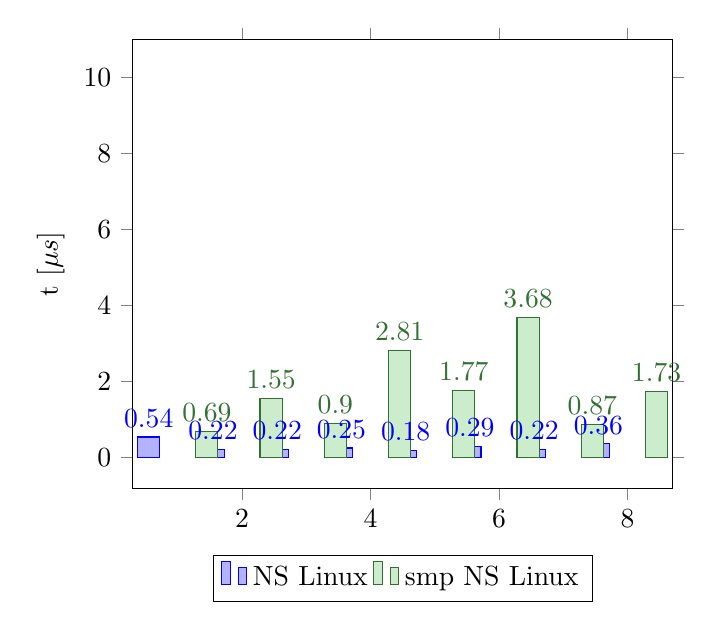
\begin{tikzpicture}
    \centering
    \begin{axis}[
    	x tick label style={
    		/pgf/number format/1000 sep=},
    	ylabel={t $[\mu s]$},
    	enlargelimits=0.1,
    	legend style={at={(0.5,-0.15)},
    	anchor=north,legend columns=-1},
      ymax=10,
    	ybar=13pt,
      bar width = 8pt,
      ytick align = outside,
      nodes near coords,
      x tick label style={rotate=0,anchor=north},
      y tick label style={rotate=0,anchor=east},
    ]
    \addplot
    	coordinates {(1,0.541) (2,0.216)
    		 (3,0.216) (4,0.252)
         (5,0.18) (6,0.289)
         (7,0.216) (8,0.36)};
    % [black!70!white,fill=black!20!white]
    \addplot[green!30!black!80!white, fill=green!65!black!20!white]
    	coordinates {(1,0.685) (2,1.549)
    		(3,0.901) (4,2.811)
        (5,1.766) (6,3.676)
        (7,0.865) (8,1.729)};
    \legend{NS Linux, \gls{smp} NS Linux}
    \end{axis}
  \end{tikzpicture}
  \caption{Odstupanje maksimalne od srednje vrijednosti vremena izvođenja \gls{smp} LTZVisora}
  \label{dev_perf}
\end{figure}
Na slici se vidi da su kod \gls{smp} LTZVisor rješenja prisutna dosta velika odstupanja maksimalnih vrijednosti od srednjih
vrijednosti vremena izvođenja, dok LTZVisor koji se izvršava na jednoj jezgri ima vrlo mala odstupanja.

\section{Performanse \gls{smp} Linux \textit{Nesigurnog} gosta}
Za procjenu performansi \textit{Nesigurnog} gosta LTZVisora, koristio se LMBench alat koji služi za testiranje raznih
aspekata sustava, uključujući latenciju i memorijsku širinu pojasa. U ovom radu su se provela dva različita testiranja:
\begin{itemize}
  \item {\textit{lat\_ops} - mjeri latenciju aritmetičkih operacija te može poslužiti kao općeniti uvid u
  performanse \gls{cpu}-a}
  \item{\textit{bw\_mem} - određuje memorijsku širinu pojasa \engl{memory bandwidth}.}
\end{itemize}
Memorijska širina pojasa je određena za razne veličine memorijskih prostora: $2~kB$, $128~kB$ i $4~MB$.
Način na koji \textit{bw\_mem} mjeri memorijsku širinu pojasa ovisi o parametru predanom od korisnika, a može biti
neki od:
\begin{itemize}
  \item{\textit{rd} - mjeri vrijeme potrebno da se pročitaju podaci konstantne vrijednosti te se podaci zbrajaju u
  konačnu sumu uz to da se pristupa svakoj četvrtoj riječi.}
  \item{\textit{wr} - mjeri vrijeme potrebno da se podaci konstantne vrijednosti upišu u polje cijelih brojeva,
  uz pristup svakoj četvrtoj riječi.}
  \item{\textit{rdwr} - mjeri vrijeme potrebno da se pročita podatak iz određene memorijske lokacije i da se upiše
  u tu istu memorijsku lokaciju. Sve pročitane vrijednosti se dodaju u sumu. Pristupa se svakoj četvrtoj riječi.}
  \item{\textit{cp} - Vrijeme potrebno da se podaci premjeste s jedne lokacije na drugu, uz pristup svakoj četvrtoj riječi.}
  \item{\textit{frd} - isto kao i \textit{rd}, ali se pristupa svakoj riječi.}
  \item{\textit{fwr} - isto kao i \textit{wr}, ali se pristupa svakoj riječi.}
  \item{\textit{fcp} - isto kao i \textit{cp}, ali se pristupa svakoj riječi.}
  \item{\textit{bzero} - koliko se brzo izvodi \textit{bzero} funkcija (za brisanje memorije).}
  \item{\textit{bcopy} - koliko se brzo izvodi \textit{bcopy} funkcija (za kopiranje memorije).}
\end{itemize}
Testiranje pristupa memoriji je izvedeno na \gls{smp} verziji LTZVisora te je uspoređeno s rezultatima dobivenim testiranjem
LTZVisora za jednu jezgru. Svaka verzija je bila testirana pomoću opcije da se za svaki test stvore dva procesa koja
izvode jednako testiranje te se izvode paralelno. Rezultati za $2~kB$, $128~kB$ i $4~MB$ dani su slikama \ref{mem_bwdt},
\ref{mem_bwdt_128} i \ref{mem_bwdt_4m}. Koordinatna os $y$ prikazuje memorijsku širinu pojasa u $MBps$.

\begin{figure}[H]
  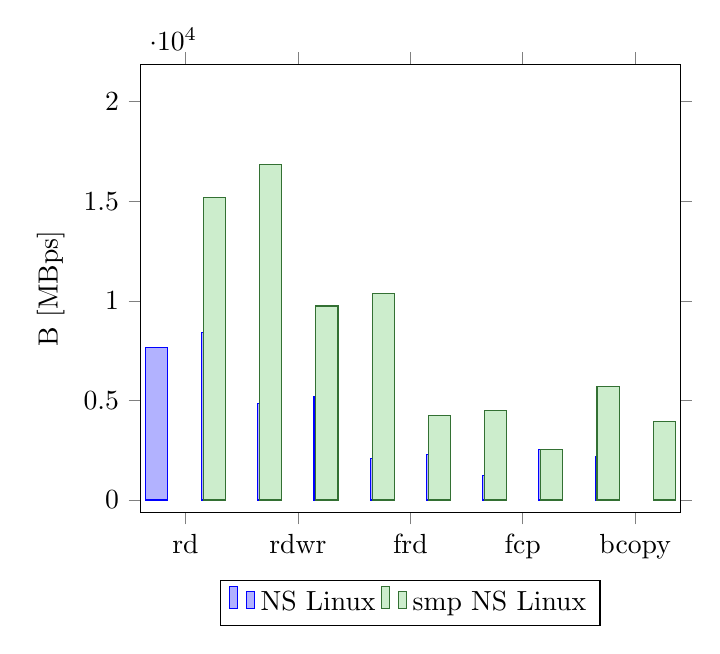
\begin{tikzpicture}
    \centering
    \begin{axis}[
    	x tick label style={
    		/pgf/number format/1000 sep=},
    	ylabel={B [MBps]},
    	enlargelimits=0.1,
    	legend style={at={(0.5,-0.15)},
    	anchor=north,legend columns=-1},
      ymax=20000,
    	ybar=13pt,
      bar width = 8pt,
      ytick align = outside,
      % nodes near coords,
      x tick label style={rotate=0,anchor=north},
      y tick label style={rotate=0,anchor=east},
      symbolic x coords = {rd,wr,rdwr,cp,frd,fwr,fcp,bzero,bcopy},
    ]
    \addplot
    	coordinates {(rd,7669) (wr,8408)
    		(rdwr,4860) (cp,5182)
        (frd,2098) (fwr,2278)
        (fcp,1248) (bzero,2514) (bcopy,2178)};
    % [black!70!white,fill=black!20!white]
    \addplot[green!30!black!80!white, fill=green!65!black!20!white]
    	coordinates {(rd,15202) (wr,16833)
    		(rdwr,9736) (cp,10368)
        (frd,4232) (fwr,4482)
        (fcp,2558) (bzero,5707) (bcopy,3956)};
    \legend{NS Linux, \gls{smp} NS Linux}
    \end{axis}
  \end{tikzpicture}
  \caption{Širina pojasa memorijskih operacija za $2~kB$}
  \label{mem_bwdt}
\end{figure}

\begin{figure}[H]
  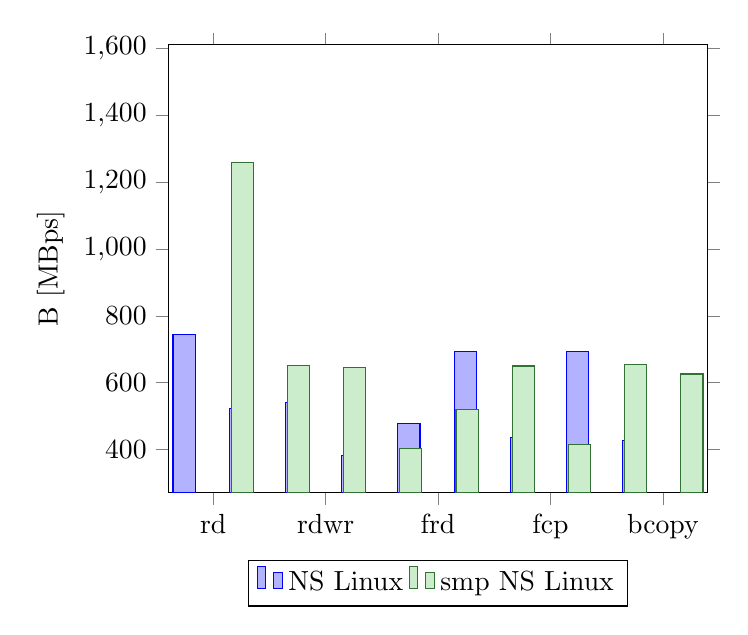
\begin{tikzpicture}
    \centering
    \begin{axis}[
    	x tick label style={
    		/pgf/number format/1000 sep=},
    	ylabel={B [MBps]},
    	enlargelimits=0.1,
    	legend style={at={(0.5,-0.15)},
    	anchor=north,legend columns=-1},
      ymax=1500,
    	ybar=13pt,
      bar width = 8pt,
      ytick align = outside,
      % nodes near coords,
      x tick label style={rotate=0,anchor=north},
      y tick label style={rotate=0,anchor=east},
      symbolic x coords = {rd,wr,rdwr,cp,frd,fwr,fcp,bzero,bcopy},
    ]
    \addplot
    	coordinates {(rd,745) (wr,524)
    		(rdwr,540) (cp,382)
        (frd,477) (fwr,692)
        (fcp,437) (bzero,693) (bcopy,428)};
    % [black!70!white,fill=black!20!white]
    \addplot[green!30!black!80!white, fill=green!65!black!20!white]
    	coordinates {(rd,1259) (wr,651)
    		(rdwr,645) (cp,402)
        (frd,519) (fwr,650)
        (fcp,415) (bzero,655) (bcopy,626)};
    \legend{NS Linux, \gls{smp} NS Linux}
    \end{axis}
  \end{tikzpicture}
  \caption{Širina pojasa memorijskih operacija za $128~kB$}
  \label{mem_bwdt_128}
\end{figure}

\begin{figure}[H]
  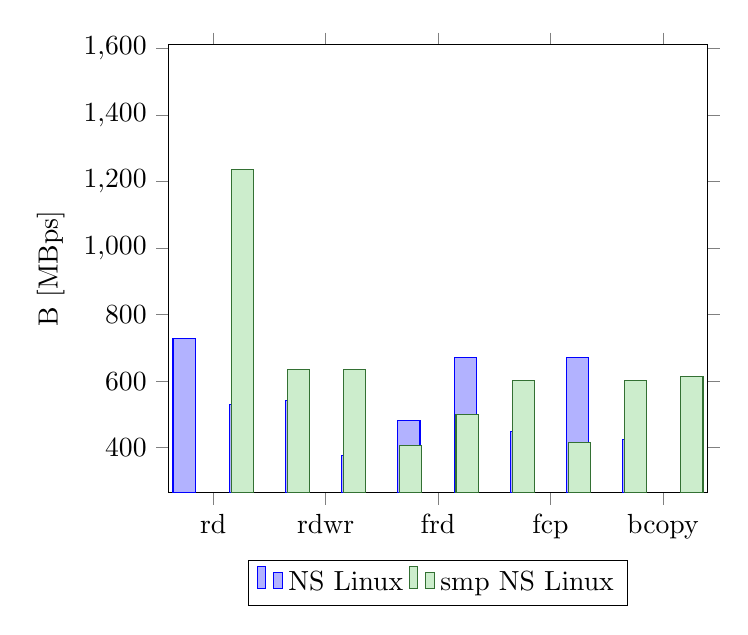
\begin{tikzpicture}
    \centering
    \begin{axis}[
    	x tick label style={
    		/pgf/number format/1000 sep=},
    	ylabel={B [MBps]},
    	enlargelimits=0.1,
    	legend style={at={(0.5,-0.15)},
    	anchor=north,legend columns=-1},
      ymax=1500,
    	ybar=13pt,
      bar width = 8pt,
      ytick align = outside,
      % nodes near coords,
      x tick label style={rotate=0,anchor=north},
      y tick label style={rotate=0,anchor=east},
      symbolic x coords = {rd,wr,rdwr,cp,frd,fwr,fcp,bzero,bcopy},
    ]
    \addplot
    	coordinates {(rd,729) (wr,531)
    		(rdwr,541) (cp,377)
        (frd,483) (fwr,670)
        (fcp,450) (bzero,672) (bcopy,425)};
    % [black!70!white,fill=black!20!white]
    \addplot[green!30!black!80!white, fill=green!65!black!20!white]
    	coordinates {(rd,1237) (wr,634)
    		(rdwr,636) (cp,406)
        (frd,499) (fwr,601)
        (fcp,416) (bzero,602) (bcopy,613)};
    \legend{NS Linux, \gls{smp} NS Linux}
    \end{axis}
  \end{tikzpicture}
  \caption{Širina pojasa memorijskih operacija za $4~MB$}
  \label{mem_bwdt_4m}
\end{figure}

Na prikazanim rezultatima, vidi se da \gls{smp} Linux u \gls{smp} LTZVisoru ima gotovo dvostruko bolje performanse od Linuxa na
jednoj jezgri (može napraviti dvostruko više pristupa memoriji od Linuxa na jednoj jezgri u jednakoj jedinici vremena)
za testiranje za $2~kB$.
Isto tako, vidi se da porastom testirane memorije performanse obje verzije Linuxa padaju. Takvo ponašanje ima smisla zato
što Linux koristi L1 i L2 \textit{cache} memorije. U dokumentaciji \textit{bw\_mem} stoji kako navedeni alat alocira
dvostruko više memorije od zadane. Dakle, ako se je za prvi slučaj zadalo $2~kB$, \textit{bw\_mem} alocira ukupno $4~kB$
za jedan proces, dok za dva procesa sveukupno zauzme $8~kB$. Navedenih $8~kB$ stane u \textit{cache} memoriju procesora
(L1 od $32~kB$ i L2 od $512~kB$). Poznato je da je \textit{cache} brza memorija te su zbog toga navedeni rezultati
očekivani (povećanjem testirane memorije, povećava se i količina memorije koja se ne nalazi u \textit{cacheu}). Isto tako,
za prvi slučaj je logično i da će \gls{smp} Linux biti vrlo visokih performansi obzirom na to da svaki procesor implementira
vlastitu L1 \textit{cache} memoriju od $32~kB$. Pad performansi \gls{smp} Linuxa u odnosu na Linux na jednoj jezgri za memoriju
veliku $4~MB$ je također razumljivo iz razloga što za razliku od L1 \textit{cache} memorije, L2 \textit{cache} memorija
je dijeljena između procesora te je na takvu količinu memorije vjerojatnije da će biti potrebno više operacija rukovanja
L2 \textit{cache} memorijom što smanjuje performanse sustava.\\
Idući rezultati se odnose na latenciju (trajanje) aritmetičkih operacija koji su dobiveni pomoću \textit{lat\_ops}
testa. Test izvodi mjerenja nad raznim vrstama operacija: zbrajanje, množenje i dijeljenje različitih vrsta podataka
(cijelih i realnih brojeva od 4 ili 8 bajta). Uz navedene operacije, test služi i za određivanje trajanja operacija
s vektorima u kojima se vidi jedina razlika između Linuxa za jednu jezgru i \gls{smp} Linuxa. Prilikom izvođenja testa,
\gls{vfp} jedinica je omogućena. Tablica \ref{vect_ops} prikazuje rezultate mjerenja operacija nad vektorima.

\begin{table}[H]
  \centering
  \caption{Trajanje operacija nad vektorima}
  \label{vect_ops}
  \begin{tabular}{|| p{4cm} | p{3.5cm} | p{3.5cm} ||}
    \hline
    \textbf{Duljina podataka} & \textbf{Trajanje u~Linuxu} & \textbf{Trajanje u \gls{smp} Linuxu} \\
    \hline\hline
    4 bajta & $41.74~ns$ & $20.94~ns$\\
    \hline
    8 bajta & $70.84~ns$ & $35.58~ns$\\
    \hline
  \end{tabular}
\end{table}

Iz rezultata je vidljivo kako \gls{smp} Linux daje dvostruko bolje rezultate od Linuxa građenog za jednu jezgru, što ima smisla
jer korištenjem dva procesora sustava, povećava se i ukupna radna frekvencija.

\chapter{Budući rad}
Da bi \gls{smp} LTZVisor rješenje bilo kvalitetno, potrebno je ukloniti mane opisane implementacije koje su već sada uočene.
Prva mana se odnosi na obradu \gls{fiq} prekida koji se može pojaviti na \gls{cpu}1. Trenutno rješenje ne nudi nikakvu obradu \gls{fiq}-a
ako se pojavi na sekundarnoj jezgri te bi bilo poželjno da \gls{fiq} bude obrađen. Daljnjim istraživanjem \gls{smp} LTZVisor
rješenja moći će se utvrditi koji mehanizam rješavanja pojave \gls{fiq}-a na \gls{cpu}1 bi bio najbolji. Sljedeće što je potrebno
za uvjerljivu demonstraciju virtualizacije pomoću LTZVisora je implementirati \gls{smp} LTZVisor s FreeRTOS
\textit{Sigurnim} gostom i \gls{smp} Linuxom \textit{Nesigurnim} gostom. Nakon što bi se navedeno implementiralo, bilo bi
potrebno i ponoviti mjerenja koja procjenjuju performanse \gls{smp} LTZVisora. Isto tako, prije ponavljanja mjerenja, trebalo
bi obratiti pažnju na uklanjanje izvora nepredvidljivosti koji je prikazan u prethodnom poglavlju. \\
Jedan ključan element
u virtualizaciji je komunikacija između virtualnih strojeva. Ovim radom je prikazan jednostavan model kojeg je potrebno
proširiti. Za te potrebe, trebalo bi proširiti implementirani sustavski poziv koji generira \gls{smc} tako da bi se
\textit{Sigurnom} gostu moglo predati i više od jednog podatka (npr. uz \gls{smc}, LTZVisoru predati i dodatne parametre koji
bi označavali početnu adresu podataka i broj podataka koje \textit{Sigurni} gost treba pročitati). Uz to, bilo bi poželjno
i da komunikacija bude dvosmjerna, tako da i \textit{Sigurni} gost može proslijediti poruku \textit{Nesigurnom} gostu.
Uz to, trebalo bi implementirati odgovarajući sinkronizacijski mehanizam koji će usmjeravati poruke odgovarajućem \gls{cpu}-u
\textit{Nesigurnog} gosta.
Predstavljeno rješenje \gls{smp} LTZVisora pripada jednom od modela predloženih od ARM-a za razvoj \textit{TrustZone} aplikacija.
Drugi model je kompleksnije za implementirati, ali takav model bi imao poseban doprinos \textit{Nesigurnom} gostu koji
bi takvim modelom imao mogućnost poboljšati efikasnost raspoređivanja zadataka te implementacija takvog modela također
spada u budući rad.

\chapter{Zaključak}
Ovim radom prikazano je kako \textit{TrustZone} doprinosi izolaciji između operacijskih sustava te kako se
mogu zaštititi osjetljivi podaci. LTZVisor je, iskorištavajući \textit{TrustZone} ekstenziju, predstavio virtualizaciju
koja nema potrebe za dodatnim virtualizacijskim ekstenzijama. Implementacija LTZVisora je također doprinijela
implementaciji dvaju operacijskih sustava koji se izvode konkurentno na jednom procesoru uz potpunu izolaciju
operacijskih sustava. Kao što je već bilo prikazano, korištenje više procesora može znatno poboljšati karakteristike
implementiranog rješenja. Tako je \gls{amp} LTZVisor poboljšao originalnu verziju LTZVisora na način da se uklonila mogućnost
da \textit{Nesigurni} gost ne dobije dovoljno procesorskog vremena od \textit{Sigurnog} gosta.\\
Predstavljeno rješenje za \gls{smp} LTZVisor je, slikovito rečeno, jedan okvir kojeg je potrebno popunit dodatnim mehanizmima
i kvalitetnijom implementacijom. Iako je rješenje nepotpuno, u prethodnim poglavljima su bile prikazane prednosti
ovakve implementacije u odnosu na originalni LTZVisor. Dakle, prikazano je kako \gls{smp} LTZVisor efikasno rješava
operacije s vektorima što ga čini dobrim rješenjem za aplikacije koje zahtijevaju izolaciju između dva operacijska
sustava uz primjenu za obradu signala. Isto tako, prikazano je kako \gls{smp} LTZVisor može pristupati memoriji efikasnije
od originalnog LTZVisora. Iako je navedeno istina, vidjelo se i da to nije točno u svim slučajevima, što ukazuje na to
da je rješenje potrebno detaljno poznavati prije nego se krene u implementaciju neke od primjena. Još jedna ključna prednost
\gls{smp} LTZVisora je da \textit{Nesigurni} gost ima mogućnost za obradu \gls{irq} prekida za vrijeme izvođenja \textit{Sigurnog}
gosta, što znatno olakšava opterećenje \textit{Nesigurnog} gosta.
\gls{smp} LTZVisor je još uvijek nepotpuno rješenje i ima prostora za raznim poboljšanjima, ali je dovoljno dobro da bude temelj
za daljnja istraživanja, nadogradnju i optimizaciju.

% \begin{appendix}
% \chapter{}
% \end{appendix}

\bibliography{literatura}
\bibliographystyle{unsrtnat}

\glsaddall
\printglossary[type=\acronymtype,title=Kazalo pojmova]

\title{Proširenje LTZVisor monitora virtualnih strojeva \\za višejezgrene procesore}
\begin{sazetak}
\textit{TrustZone} je sigurnosna ekstenzija ARM-a koja već dugi niz godina pruža sigurnosnu podršku Cortex-A procesorima.
Navedena ekstenzija pruža koncept \textit{Sigurnog} \engl{Secure} i \textit{Nesigunog} \engl{Non-Secure} svijeta.
Svaki svijet se može izvršavati na jednom procesoru metodom vremenske podijele, što omogućava implementaciju
dvaju operacijskih sustava. LTZVisor (\textit{Leightweight TrustZone hypervisor}) je monitor virtualnih strojeva koji
iskorištava \textit{TrustZone} ekstenziju. Namjena LTZVisora je da implementira gotovo rješenje za
upravljanje s resursima potrebnim operacijskom sustavu koji se izvršava u \textit{Sigurnom} svijetu i resursima
potrebnima operacijskom sustavu \textit{Nesigurnog} svijeta. Početna verzija LTZVisora bila je namijenjena jednom
procesoru te se je ubrzo razvila i \gls{amp} \engl{Asymmetric Multiprocessing} verzija LTZVisora koja omogućava da se
\textit{Nesigurni} gost i \textit{Sigurni} gost izvode paralelno (bez potrebe za metodom vremenske podijele), svaki na
svojoj jezgri.
Ovaj rad po prvi puta predstavlja \gls{smp} \engl{Symmetric Multiprocessing} LTZVisor verziju koja, prema preporukama ARM-a,
implementira rješenje u kojem se \textit{Sigurni} gost izvršava na jednoj jezgri, a \textit{Nesigurni} gost u \gls{smp}
konfiguraciji. U radu je opisan jednostavan model komunikacije za potrebe demonstracije funkcionalnog rješenja
\gls{smp} LTZVisora, gdje se jasno pokazuje kako \textit{Nesigurni} gost radi u \gls{smp} konfiguraciji. Na kraju, dana su
razna mjerenja za evaluaciju implementiranog rješenja.

\kljucnerijeci{\textit{TrustZone}, \textit{Siguran} svijet, \textit{Nesiguran} svijet, LTZVisor, \gls{amp}, \gls{smp}}
\end{sazetak}

% TODO: Navedite naslov na engleskom jeziku.
\newpage
\engtitle{Extending LTZVisor Hypervisor to Multicore Processors}
\begin{abstract}
For a long time, the ARM company provides security support by implementing TrustZone security extensions in Cortex-A processors.
The security extension enables the concept of the Secure and Non-Secure world. Each of the worlds can be executed on one
processor in time-sliced fashion. This fact can be used to implement two operating systems, each for one world. LTZVisor
(Leightweight TrustZone hypervisor) is a simple hypervisor that exploits TrustZone security extensions. Implementation
of the LTZVisor is a complete solution that enables managing of resources needed by Secure and Non-Secure virtual machines.
LTZVisor was originally implemented for one core, but soon after implementing the original LTZVisor, \gls{amp} (Asymmetric
Multiprocessing) version of LTZVisor was introduced. \gls{amp} LTZVisor enabled the possibility of parallel execution of
Secure and Non-Secure virtual machines, each machine for one core. This thesis, for the first time, introduces the \gls{smp}
(Symmetric Multiprocessing) version of LTZVisor, which follows ARM's recommendations for implementation of \gls{smp} TrustZone
applications. \gls{smp} LTZVisor enables the possibility to execute \gls{smp} software in Non-Secure world, while Secure world still
executes on one core. The thesis introduces a simple communication model with purpose of demonstrating a functional
\gls{smp} LTZVisor solution where it can clearly be seen that Non-Secure executes in \gls{smp} fashion. To evaluate implemented
solution, \gls{smp} LTZVisor was put under a range of tests to show advantages and drawbacks of using \gls{smp} LTZVisor.

\keywords{TrustZone, Secure world, Non-Secure world, LTZVisor, \gls{amp}, \gls{smp}}
\end{abstract}

\end{document}
